%%%%%%%%%%%%%%%%%%%%%%%%%%%%%%%%%%%%%%%%%%%%%%%%%%%%%%%%%%%%%%%%%%%%%%%%%%%
%
% Generic template for TFC/TFM/TFG/Tesis
%
% $Id: book.tex,v 1.13 2014/01/11 23:27:55 macias Exp $
%
% By:
%  + Javier Mac�as-Guarasa.
%    Departamento de Electr�nica
%    Universidad de Alcal�
%  + Roberto Barra-Chicote.
%    Departamento de Ingenier�a Electr�nica
%    Universidad Polit�cnica de Madrid
%
% Based on original sources by Roberto Barra, Manuel Oca�a, Jes�s Nuevo,
% Pedro Revenga, Fernando Herr�nz and Noelia Hern�ndez. Thanks a lot to
% all of them, and to the many anonymous contributors found (thanks to
% google) that provided help in setting all this up.
%
% See also the additionalContributors.txt file to check the name of
% additional contributors to this work.
%
% If you think you can add pieces of relevant/useful examples,
% improvements, please contact us at (macias@depeca.uah.es)
%
% Copyleft 2013
%
%%%%%%%%%%%%%%%%%%%%%%%%%%%%%%%%%%%%%%%%%%%%%%%%%%%%%%%%%%%%%%%%%%%%%%%%%%%

% This is for rubber to clean additional files
% rubber: clean book.acn book.acr book.alg book.cod book.ist book.out book.sbl book.slg book.sym book.lor

%%%%%%%%%%%%%%%%%%%%%%%%%%%%%%%%%%%%%%%%%%%%%%%%%%%%%%%%%%%%%%%%%%%%%%%%%%%
% BEGIN Preamble and configuration section
%
\input{config/preamble.tex}    % DO NOT TOUCH THIS LINE. You can edit
                               % the file to modify some default settings

%%%%%%%%%%%%%%%%%%%%%%%%%%%%%%%%%%%%%%%%%%%%%%%%%%%%%%%%%%%%%%%%%%%%%%%%%%%
%
% Generic template for TFC/TFM/TFG/Tesis
%
% $Id: myconfig.tex,v 1.10 2014/01/20 10:06:29 macias Exp $
%
% By:
%  + Javier Mac�as-Guarasa. 
%    Departamento de Electr�nica
%    Universidad de Alcal�
%  + Roberto Barra-Chicote. 
%    Departamento de Ingenier�a Electr�nica
%    Universidad Polit�cnica de Madrid   
% 
% Based on original sources by Roberto Barra, Manuel Oca�a, Jes�s Nuevo,
% Pedro Revenga, Fernando Herr�nz and Noelia Hern�ndez. Thanks a lot to
% all of them, and to the many anonymous contributors found (thanks to
% google) that provided help in setting all this up.
%
% See also the additionalContributors.txt file to check the name of
% additional contributors to this work.
%
% If you think you can add pieces of relevant/useful examples,
% improvements, please contact us at (macias@depeca.uah.es)
%
% Copyleft 2013
%
%%%%%%%%%%%%%%%%%%%%%%%%%%%%%%%%%%%%%%%%%%%%%%%%%%%%%%%%%%%%%%%%%%%%%%%%%%%

%%%%%%%%%%%%%%%%%%%%%%%%%%%%%%%%%%%%%%%%%%%%%%%%%%%%%%%%%%%%%%%%%%%%%%%%%%% 
%
% Contents of this file:
% + Definition of variables controlling compilation flavours
% + Definition of your own commands (samples provided)
%
% You must edit it to suit to your specific case
%
% Specially important are the definition of your variables (title of the
% book, your degree, author name, email, advisors, keywords (in Spanish
% and English), year, ... They will be used in generating the adequate
% front and cover pages, automagically.
%
%%%%%%%%%%%%%%%%%%%%%%%%%%%%%%%%%%%%%%%%%%%%%%%%%%%%%%%%%%%%%%%%%%%%%%%%%%% 

%%%%%%%%%%%%%%%%%%%%%%%%%%%%%%%%%%%%%%%%%%%%%%%%%%%%%%%%%%%%%%%%%%%%%%%%%%% 
% BEGIN Set my own variables (control compilation for different flavours)

% Control language specific modifications
% This can be english or spanish
\newcommand{\mybooklanguage}{spanish}

% Control compilation flavour (for PFCs, TFMs, TFGs, Thesis, etc...)
% Degree (titulaci�n), can be:
% IT     - Ingenier�a de Telecomunicaci�n
% IE     - Ingenier�a Electr�nica
% ITTSE  - Ingenier�a T�cnica de Telecomunicaci�n, Sistemas Electr�nicos
% ITTST  - Ingenier�a T�cnica de Telecomunicaci�n, Sistemas de Telecomunicaci�n
% ITI    - Ingenier�a T�cnica Industrial, Electr�nica Industrial 
% GIEC   - Grado en Ingenier�a Electr�nica de Comunicaciones
% GIEAI  - Grado en Ingenier�a en Electr�nica y Autom�tica Industrial
% GIST   - Grado en Ingenier�a en Sistemas de Telecomunicaci�n
% GITT   - Grado en Ingenier�a en Tecnolog�as de la Telecomunicaci�n
% GIT    - Grado en Ingenier�a Telem�tica
% GIC    - Grado en Ingenier�a de Computadores
% GII    - Grado en Ingenier�a Inform�tica
% GSI    - Grado en Sistemas de Informaci�n
% MUSEA  - M�ster Universitario en Sistemas Electr�nicos Avanzados. Sistemas Inteligentes
% PHDUAH - Doctorado UAH
% PHDUPM - Doctorado UPM
% You can include additional degrees and modify config/myconfig.tex
% config/postamble.tex and cover/cover.tex, generating new specific
% cover files if needed
\newcommand{\mydegree}{IE}

% General document information
\newcommand{\mybooktitle}{Manual de referencia para el desarrollo de robots de Eurobot}
\newcommand{\mybookauthor}{Javier Bali�as Santos}
\newcommand{\mybookdepartment}{Departamento de Electr�nica}
\newcommand{\mybookschool}{Escuela Polit�cnica Superior}
\newcommand{\mybookuniversity}{Universidad de Alcal�}
\newcommand{\mybookauthordegree}{Ingeniero de Electronica} % Used in UPM
\newcommand{\mybookemail}{balinas@gmail.com}
\newcommand{\mybookadvisors}{Julio Pastor Mendoza}
\newcommand{\mybookpresident}{Name of the tribunal president}
\newcommand{\mybookfirstvocal}{Name of the first vocal}
\newcommand{\mybooksecondvocal}{Name of the second vocal}
\newcommand{\mybooksecretary}{Name of the secretary (if needed)}
\newcommand{\mybookyear}{2016}
\newcommand{\myanteproyectodate}{1 de diciembre de 2015}
\newcommand{\mybookkeywords}{Eurobot robots, reference manual, management, electronics, mechanics, software} % (up to a maximum of five)
\newcommand{\mybookpalabrasclave}{robot, Eurobot, din�mica, hardware, mec�nica, software, microcontrolador, simulador} % (m�ximo de cinco)

% Link color definition
% Color links of the toc/lot/lof entries
\newcommand{\mytoclinkcolor}{azul}
\newcommand{\myloflinkcolor}{rojo}
\newcommand{\mylotlinkcolor}{verde}
% This is used in cover/extralistings.tex
\newcommand{\myothertoclinkcolor}{magenta}

% Other color links in the document
\newcommand{\mylinkcolor}{azul}
%\newcommand{\mylinkcolor}{negro}

% Color links to urls and cites
\newcommand{\myurlcolor}{azul}
\newcommand{\mycitecolor}{verde}

% END Set my own variables (control compilation for different flavours)
%%%%%%%%%%%%%%%%%%%%%%%%%%%%%%%%%%%%%%%%%%%%%%%%%%%%%%%%%%%%%%%%%%%%%%%%%%% 

%%%%%%%%%%%%%%%%%%%%%%%%%%%%%%%%%%%%%%%%%%%%%%%%%%%%%%%%%%%%%%%%%%%%%%%%%%% 
% BEGIN My own commands section 
% Define your own commands here

% This one is to define a specific format for english text in a Spanish
% document
\DeclareRobustCommand{\texten}[1]{\textit{#1}}

% Various examples of commonly used commands
\newcommand{\circulo}{\large $\circ$}
\newcommand{\asterisco}{$\ast$}
\newcommand{\cuadrado}{\tiny $\square$}
\newcommand{\triangulo}{\scriptsize $\vartriangle$}
\newcommand{\triangv}{\scriptsize $\triangledown$}
\newcommand{\diamante}{\large $\diamond$}

\newcommand{\new}[1]{\textcolor{magenta}{#1 }}
\newcommand{\argmax}[1]{\underset{#1}{\operatorname{argmax}}}

% END My own commands section 
%%%%%%%%%%%%%%%%%%%%%%%%%%%%%%%%%%%%%%%%%%%%%%%%%%%%%%%%%%%%%%%%%%%%%%%%%%% 

%%% Local Variables:
%%% TeX-master: "../book"
%%% End:


    % DO NOT TOUCH THIS LINE, but EDIT THIS FILE
                               % to set your specific settings (related
                               % to the document language, your degree,
                               % document details (such as title, author
                               % (you), your email, name of the tribunal
                               % members, document year, keyword and
                               % palabras clave) and link colors), and
                               % define your commonly used commands
                               % (some examples are provided).

\input{config/glossaries.tex}  % EDIT THIS FILE to include your glossaries

\input{config/postamble.tex}   % DO NOT TOUCH THIS LINE. Yes, I know,
                               % "postamble" is not a valid word... :-)

% path to directories containing images
\graphicspath{{./logos/}{./figures/}{./diagrams/}} % Edit this to your
                                % needs. Only logos is really required
                                % when you generate your own content.
%
% END Preamble and configuration section
%%%%%%%%%%%%%%%%%%%%%%%%%%%%%%%%%%%%%%%%%%%%%%%%%%%%%%%%%%%%%%%%%%%%%%%%%%%

%%%%%%%%%%%%%%%%%%%%%%%%%%%%%%%%%%%%%%%%%%%%%%%%%%%%%%%%%%%%%%%%%%%%%%%%%%%
% Let's start with the real stuff
%%%%%%%%%%%%%%%%%%%%%%%%%%%%%%%%%%%%%%%%%%%%%%%%%%%%%%%%%%%%%%%%%%%%%%%%%%%
\begin{document}

%%%%%%%%%%%%%%%%%%%%%%%%%%%%%%%%%%%%%%%%%%%%%%%%%%%%%%%%%%%%%%%%%%%%%%%%%%%
% Now start text and numbering for frontmatter (toc, list of
% tables/figures,...)
%%%%%%%%%%%%%%%%%%%%%%%%%%%%%%%%%%%%%%%%%%%%%%%%%%%%%%%%%%%%%%%%%%%%%%%%%%%
\frontmatter                                  % DO NOT TOUCH THIS LINE

%%%%%%%%%%%%%%%%%%%%%%%%%%%%%%%%%%%%%%%%%%%%%%%%%%%%%%%%%%%%%%%%%%%%%%%%%%%
% BEGIN within-document configuration, frontpage and cover pages generation
%

% Set Language dependent issues that must be set after \begin{document}
\input{config/setlanguagedependentissues.tex} % DO NOT TOUCH THIS LINE
                                              % NOR THE FILE

% This will include front page (if needed), and cover pages. Selection
% of the adequate one is done automagically depending on values set by
% the user in config/myconfig.tex
\input{cover/cover.tex}                       % DO NOT TOUCH THIS
                                              % LINE/FILE. You can edit
                                              % the file in case you
                                              % need it (there may be
                                              % problems with vertical
                                              % spacing if the title is
                                              % too long...)


%%%%%%%%%%%%%%%%%%%%%%%%%%%%%%%%%%%%%%%%%%%%%%%%%%%%%%%%%%%%%%%%%%%%%%%%%%%
% In some cases you may need to include pdf files (for example in the
% PhD. Thesis at UAH you need to include the permission letter by the
% advisors...). You can do this
%
%\includepdf[pages=3-4]{letters/sampleLetter-pages.pdf} % include pages
%                                                       % 3-4 of pdf file
%\clearemptydoublepage % You need to include this after including each pdf

%\includepdf[pages=-]{letters/sampleLetter.pdf}   % include all pages of
%                                                 % pdf file
%\clearemptydoublepage % You need to add this after including each pdf

% Dedication+ackowledgements (dedicatorias+agradecimientos)
%%%%%%%%%%%%%%%%%%%%%%%%%%%%%%%%%%%%%%%%%%%%%%%%%%%%%%%%%%%%%%%%%%%%%%%%%%%
%
% Generic template for TFC/TFM/TFG/Tesis
%
% $Id: dedicatoria.tex,v 1.3 2014/01/08 22:56:06 macias Exp $
%
% By:
%  + Javier Mac�as-Guarasa. 
%    Departamento de Electr�nica
%    Universidad de Alcal�
%  + Roberto Barra-Chicote. 
%    Departamento de Ingenier�a Electr�nica
%    Universidad Polit�cnica de Madrid   
% 
% Based on original sources by Roberto Barra, Manuel Oca�a, Jes�s Nuevo,
% Pedro Revenga, Fernando Herr�nz and Noelia Hern�ndez. Thanks a lot to
% all of them, and to the many anonymous contributors found (thanks to
% google) that provided help in setting all this up.
%
% See also the additionalContributors.txt file to check the name of
% additional contributors to this work.
%
% If you think you can add pieces of relevant/useful examples,
% improvements, please contact us at (macias@depeca.uah.es)
%
% Copyleft 2013
%
%%%%%%%%%%%%%%%%%%%%%%%%%%%%%%%%%%%%%%%%%%%%%%%%%%%%%%%%%%%%%%%%%%%%%%%%%%%

%
% This is also courtesy of Roberto Barra
%
\thispagestyle{empty}

\begin{flushright}

  \textbf{} \\
  \vspace{6cm}
  % \hspace{7.3cm}

  \textbf{A mis padres. Maritere y Julio}\\
  \vspace{3cm}
  \hspace{8cm}
  %\emph{``Empieza haciendo lo necesario, luego haz lo posible y de pronto empezar�s a hacer lo imposible.''}\\ Francisco de As�s

\end{flushright}  

% \clearemptydoublepage



%%% Local Variables:
%%% TeX-master: "../book"
%%% End:
            % EDIT this file or
                                              % comment it out
%%%%%%%%%%%%%%%%%%%%%%%%%%%%%%%%%%%%%%%%%%%%%%%%%%%%%%%%%%%%%%%%%%%%%%%%%%%
%
% Generic template for TFC/TFM/TFG/Tesis
%
% $Id: agradecimientos.tex,v 1.5 2014/01/10 10:06:23 macias Exp $
%
% By:
%  + Javier Mac�as-Guarasa. 
%    Departamento de Electr�nica
%    Universidad de Alcal�
%  + Roberto Barra-Chicote. 
%    Departamento de Ingenier�a Electr�nica
%    Universidad Polit�cnica de Madrid   
% 
% Based on original sources by Roberto Barra, Manuel Oca�a, Jes�s Nuevo,
% Pedro Revenga, Fernando Herr�nz and Noelia Hern�ndez. Thanks a lot to
% all of them, and to the many anonymous contributors found (thanks to
% google) that provided help in setting all this up.
%
% See also the additionalContributors.txt file to check the name of
% additional contributors to this work.
%
% If you think you can add pieces of relevant/useful examples,
% improvements, please contact us at (macias@depeca.uah.es)
%
% Copyleft 2013
%
%%%%%%%%%%%%%%%%%%%%%%%%%%%%%%%%%%%%%%%%%%%%%%%%%%%%%%%%%%%%%%%%%%%%%%%%%%%

\ifthenelse{\equal{\mybooklanguage}{english}}
{
  \chapter*{Acknowledgements}
  \label{cha:acknowledgements}
  \markboth{Acknowledgements}{Acknowledgements}
}
{
  \chapter*{Agradecimientos}
  \label{cha:agradecimientos}
  \markboth{Agradecimientos}{Agradecimientos}
}

% Use this if you don't like the fancy style
\thispagestyle{myplain}



\begin{FraseCelebre}
  \begin{Frase}
    M�s vale un minuto de ilusi�n que mil horas de razonamiento.
  \end{Frase}
  \begin{Fuente}
    Roberto Barra-Chicote
  \end{Fuente}
\end{FraseCelebre}


Este trabajo y sobre todo lo que expone es fruto de muchas horas de trabajo y esfuerzo de muchas personas. En lo que me ata�e, me gustar�a agradecer a todas las personas que me han acompa�ado, apoyado y que han sido parte de cada uno de los robots en los que he estado implicado.

Agradecer a Julio la iniciativa de crear all� por el a�o 2003 un equipo de Eurobot. Igualmente agradecerle el apoyo, ayuda e implicaci�n en los equipos de Eurobot que se formaron desde entonces. Tambi�n me gustar�a aprovechar para felicitarle por el esfuerzo, la constancia y la tenacidad en el promover las competiciones de rob�tica desde la Universidad de Alcal�. Una de ellas me marc� el camino y estoy seguro que el de mucha m�s gente.

Es curioso, en mi cabeza los a�os tienen nombre de robot. Y cada robot lo asocio con la gente que form�bamos el equipo que lo construimos. Mi agradecimiento a todos y cada uno por los buenos y malos momentos vividos, entre todos, los malos fueron se soportaron mejor y lo buenos fueron m�s grandiosos.  Especialmente mi agradecimiento a aquellos que sent� m�s cerca y con los que compart� m�s momentos: Diego Alonso, Kike, Jose, Saleta, Oscar, Marcelo, Sergio y Nilo.

Agradecer tambi�n a mis �ltimos compa�eros del equipo Eurobotics Engineering: Carlos, Rub�n, Silvia y Javi. Formamos un buen equipo y vivimos grandes aventuras, especialmente el �ltimo a�o. Las ganas e ilusi�n de todos vosotros me ayudaron a seguir en momentos de flaqueza. Sobre todo en el �ltimo a�o, gracias a Javi por su esp�ritu de equipo, sus ganas, iniciativa y constantes mensajes de �nimo al equipo.

Me gustar�a hacer una menci�n muy especial a Diego y Mario. Sin ellos no hubiera sido posible hacer todo lo que hemos hecho y llegar hasta donde hemos llegado en todos estos a�os. Gracias a Diego por tus ganas, esfuerzo e �mpetu sincero que nos hizo llegar alto, los mismos que ahora te hacen recorrer monta�as por el mundo. Gracias a Mario que siempre, siempre, siempre, has estado apoyando e implic�ndote en todos los robots, sacando tiempo de donde no lo ten�as. Gracias amigo.

Un recordatorio especial a Guillermo, gracias por tu apoyo incondicional durante todos estos a�os. S�lo tu capacidad de asombro por los robots he hemos hecho, hac�a que mereciese la pena todo el esfuerzo. Se te recordar� siempre.

Por �ltimo, agradecer a las personas que directamente o indirectamente han sufrido mis ausencias por mi dedicaci�n a los robots, mi familia y amigos. Especialmente agradecer a Jana su apoyo, paciencia y esfuerzo por comprenderme.



% Back to normal JIC. Use it if you set \pagestyle{myplain} above
%\pagestyle{fancy}

%%% Local Variables:
%%% TeX-master: "../book"
%%% End:


  % EDIT this file or
                                              % comment it out

% Now include resumen and abstract
%%%%%%%%%%%%%%%%%%%%%%%%%%%%%%%%%%%%%%%%%%%%%%%%%%%%%%%%%%%%%%%%%%%%%%%%%%%
%
% Generic template for TFC/TFM/TFG/Tesis
%
% $Id: resumen.tex,v 1.7 2014/01/08 22:56:02 macias Exp $
%
% By:
%  + Javier Mac�as-Guarasa. 
%    Departamento de Electr�nica
%    Universidad de Alcal�
%  + Roberto Barra-Chicote. 
%    Departamento de Ingenier�a Electr�nica
%    Universidad Polit�cnica de Madrid   
% 
% Based on original sources by Roberto Barra, Manuel Oca�a, Jes�s Nuevo,
% Pedro Revenga, Fernando Herr�nz and Noelia Hern�ndez. Thanks a lot to
% all of them, and to the many anonymous contributors found (thanks to
% google) that provided help in setting all this up.
%
% See also the additionalContributors.txt file to check the name of
% additional contributors to this work.
%
% If you think you can add pieces of relevant/useful examples,
% improvements, please contact us at (macias@depeca.uah.es)
%
% Copyleft 2013
%
%%%%%%%%%%%%%%%%%%%%%%%%%%%%%%%%%%%%%%%%%%%%%%%%%%%%%%%%%%%%%%%%%%%%%%%%%%%

\chapter*{Resumen}
\label{cha:resumen}
\markboth{Resumen}{Resumen}

\addcontentsline{toc}{chapter}{Resumen}

Este trabajo de fin de carrera trata sobre el desarrollo de robots para la competici�n de robots Eurobot \cite{eurobot}. Pretende ser un manual de referencia para todo aquel que quiera construir un robot para participar en Eurobot. El trabajo est� basado en la experiencia adquirida en el desarrollo de este tipo de robots entre entre los a�os 2003 y 2015. Especialmente en el periodo entre 2010 y 2015.

Eurobot es una competici�n internacional cuyas reglas y tem�tica el juego cambian cada a�o. El libro describe la mecanica, hardware y software relativos al desarrollo e implementaci�n de las diferentes funcionalidades de un robot de Eurobot, las cuales se han dividido en dos partes principales: la \emph{plataforma rob�tica base} y los \emph{sistemas mec�nicos} de manipulaci�n de elementos del juego.

La plataforma rob�tica se basa en un \emph{sistema de tracci�n diferencial} que implementa un \emph{posicionamiento por odometr�a} y un \emph{control de posici�n polar}. La plataforma, adem�s, utiliza sensores para detectar obstaculos y un \emph{sistema de balizas} para la medir la posici�n de los robots oponentes, a partir del cual se implementa la \emph{evitaci�n de obst�culos}.

Mediante el estudio del modelo din�mico de la plataforma rob�tica se determinan los l�mites de aceleraci�n y velocidad, a partir de los cuales, dimensionar y especificar los elementos mec�nicos y estructura de la misma.

El desarrollo \emph{hardware} implementa una \emph{arquitectura} que permite ser reutilizada en el desarrollo de nuevos robots de Eurobot. Se trata de un sistema embebido basado en \emph{microcontroladores dsPIC} que reparte sus recursos entre la implementaci�n de la plataforma rob�tica y los sistema mec�nicos.

El desarrollo \emph{software} tambi�n est� basado en una \emph{arquitectura} pensada para ser reutilizada. �sta se organiza en capas y/o m�dulos funcionales con diferentes niveles de abstraci�n. El desarrollo software, incluye adem�s, un \emph{simulador de los robots y del campo de juego}. El entorno de simulaci�n permite visualizar los movimientos de los robots sobre un campo de juego virtual y simular robots oponentes.
 

\textbf{Palabras clave:} \mybookpalabrasclave.

%%% Local Variables:
%%% TeX-master: "../book"
%%% End:


                  % EDIT this file
%%%%%%%%%%%%%%%%%%%%%%%%%%%%%%%%%%%%%%%%%%%%%%%%%%%%%%%%%%%%%%%%%%%%%%%%%%%
%
% Generic template for TFC/TFM/TFG/Tesis
%
% $Id: abstract.tex,v 1.7 2014/01/08 22:56:02 macias Exp $
%
% By:
%  + Javier Mac�as-Guarasa. 
%    Departamento de Electr�nica
%    Universidad de Alcal�
%  + Roberto Barra-Chicote. 
%    Departamento de Ingenier�a Electr�nica
%    Universidad Polit�cnica de Madrid   
% 
% Based on original sources by Roberto Barra, Manuel Oca�a, Jes�s Nuevo,
% Pedro Revenga, Fernando Herr�nz and Noelia Hern�ndez. Thanks a lot to
% all of them, and to the many anonymous contributors found (thanks to
% google) that provided help in setting all this up.
%
% See also the additionalContributors.txt file to check the name of
% additional contributors to this work.
%
% If you think you can add pieces of relevant/useful examples,
% improvements, please contact us at (macias@depeca.uah.es)
%
% Copyleft 2013
%
%%%%%%%%%%%%%%%%%%%%%%%%%%%%%%%%%%%%%%%%%%%%%%%%%%%%%%%%%%%%%%%%%%%%%%%%%%%

\chapter*{Abstract}
\label{cha:abstract}

\addcontentsline{toc}{chapter}{Abstract}

%Este trabajo de fin de carrera trata sobre el desarrollo de robots para la competici�n de robots Eurobot \cite{eurobot}. Pretende ser un manual de referencia, para todo aquel que quiera construir un robot para participar en Eurobot, basado en la experiencia adquirida en el desarrollo de este tipo de robots entre entre los a�os 2003 y 2015. Especialmente en el periodo entre 2010 y 2015.

This End of Degree Assignment is about the development of robots for the Eurobot contest \cite{eurobot}. It aims to be a reference manual for whom wants to make a robot for participating on Eurobot contest. It's based on the gathered experience on the development of this kind of robots between the years 2003 and 2015. Specially on the period from 2010 to 2015.

%Eurobot es una competici�n internacional cuyas reglas y tem�tica el juego cambian cada a�o. El libro describe la mecanica, hardware y software relativos al desarrollo e implementaci�n de las diferentes funcionalidades de un robot de Eurobot, las cuales se han dividido en dos partes principales: la \emph{plataforma rob�tica base} y los \emph{sistemas mec�nicos} de manipulaci�n de elementos del juego.

Eurobot is an international contest whose theme and rules change every year. The book describes the mechanics, hardware and software related to the implementation of the different funicionalities of a robot. The implementation of these functionalities has divided in two main parts: the \emph{robotic base platform} and the \emph{mechanical systems} for the handling of game elements.

%La plataforma rob�tica se basa en un \emph{sistema de tracci�n diferencial} que implementa un \emph{posicionamiento por odometr�a} y un \emph{control de posici�n polar}. La plataforma, adem�s, utiliza sensores para detectar obstaculos y un \emph{sistema de balizas} para la medir la posici�n de los robots oponentes, a partir del cual se implementa la \emph{evitaci�n de obst�culos}.

The robotic platform is based on a \emph{differential drive system} which implements a \emph{position dead reckoning by odometry} and a \emph{polar position control}. The platform uses also sensors for the obstacles detection and a \emph{beacon system} in order to measure the opponents robots position. Using the information of the beacon system the robot implemnts an \emph{obstacle avoidance algorithm}.

%Mediante el estudio del modelo din�mico de la plataforma rob�tica se determinan los l�mites de aceleraci�n y velocidad, a partir de los cuales, dimensionar y especificar los elementos mec�nicos y estructura de la misma.

The acceleration and speed limits of the robotic platform have been determined via the study of its dinamic model. These limits are used to specify the mechanical elements and the structure of the robotic platform.

%El desarrollo hardware implementa una \textbf{arquitectura} que permite ser reutilizada en el desarrollo de nuevos robots de Eurobot. Se trata de un sistema embebido basado en \emph{microcontroladores dsPIC} que reparte sus recursos entre la implementaci�n de la plataforma rob�tica y los sistema mec�nicos.

The \emph{hardware} development implements an \emph{architecture} which can be reused on others developments of Eurobot robots. It's a embedded system based on \emph{dsPIC microcontrollers}. The system distributes its resources between the implementations of the robotic platform and the mechanical systems.


%El software desarrollado tambi�n est� basado en una arquitectura pensada para ser reutilizada. �sta se organiza en capas y/o m�dulos funcionales con diferentes niveles de abstraci�n. El m�dulo \emph{plataforma rob�tica} incluye las funcionalidades de desplazamiento, localizaci�n y evitaci�n de obst�culos. Al mismo nivel, se encuentra el m�dulo \emph{sistemas mec�nicos} encargado de controlar los mecanismos utilizados por el robot para manipular los elementos de juego. Ambos m�dulos se integran y se sincronizan en la capa de \emph{tem�tica de juego} para implementar funcionalidades propias de la tem�tica de Eurobot. Por �ltimo, la capa \emph{estrat�gia de juego} decide cuando y que acciones del juego realizar en cada momento para jugar un partido de Eurobot.

The developed \emph{software} is also based on an \emph{architecture} aimed to be reused. This architecture is organized in layers and/or functional modules with different abstraction levels. %The \emph{robotic platform level} includes the functionalities of navigation, localizaci�n and obstacle avoiding. At the same level, the \emph{mechanical systems layer} is in charge of the control of the mechanics used by the robot to manipulate the game elements. Both modules are integrated and syncronized by the \emph{game theme layer}, which implements the specific functionalities of the Eurobot theme. Finally, the \emph{game strategy layer} decides when and which actions of the game to do in each time in order to play an Eurobot match.


%El desarrollo software, incluye adem�s, un \emph{simulador de los robots y del campo de juego}. Este simulador se implementa a partir de la compilaci�n del c�digo fuente de los robots en un \emph{host} GNU/Linux y de la emulaci�n del hardware y elementos mec�nicos del robot. El entorno de simulaci�n permite visualizar los movimientos de los robots sobre un campo de juego virtual y simular robots oponentes.


The software development includes also a \emph{simulator of the robots and of the game field}. This simulator is implemented by the compilation of the robot source code on a GNU/Linux host and the emulation of the hardware and mechanical elements of the robot. The simulation enviroment allow to visualize the robot movements on a virtual game field and simulate opponents robots.

\textbf{Keywords:} \mybookkeywords.

%%% Local Variables:
%%% TeX-master: "../book"
%%% End:


                 % EDIT this file

% Just for TFGs/PFCs at UAH, I do nothing and leave to the author the
% inclusion of the file
%%%%%%%%%%%%%%%%%%%%%%%%%%%%%%%%%%%%%%%%%%%%%%%%%%%%%%%%%%%%%%%%%%%%%%%%%%%
%
% Generic template for TFC/TFM/TFG/Tesis
%
% $Id: resumen-extendido.tex,v 1.5 2014/01/08 22:56:02 macias Exp $
%
% By:
%  + Javier Mac�as-Guarasa. 
%    Departamento de Electr�nica
%    Universidad de Alcal�
%  + Roberto Barra-Chicote. 
%    Departamento de Ingenier�a Electr�nica
%    Universidad Polit�cnica de Madrid   
% 
% Based on original sources by Roberto Barra, Manuel Oca�a, Jes�s Nuevo,
% Pedro Revenga, Fernando Herr�nz and Noelia Hern�ndez. Thanks a lot to
% all of them, and to the many anonymous contributors found (thanks to
% google) that provided help in setting all this up.
%
% See also the additionalContributors.txt file to check the name of
% additional contributors to this work.
%
% If you think you can add pieces of relevant/useful examples,
% improvements, please contact us at (macias@depeca.uah.es)
%
% Copyleft 2013
%
%%%%%%%%%%%%%%%%%%%%%%%%%%%%%%%%%%%%%%%%%%%%%%%%%%%%%%%%%%%%%%%%%%%%%%%%%%%

\ifthenelse{\equal{\mybooklanguage}{english}}
{
\chapter*{Extended Abstract}
\label{cha:resumen-extendido}
\markboth{Extended Abstract}{Extended Abstract}

\addcontentsline{toc}{chapter}{Extended Abstract}
}
{
\chapter*{Resumen extendido}
\label{cha:resumen-extendido}
\markboth{Resumen extendido}{Resumen extendido}

\addcontentsline{toc}{chapter}{Resumen extendido}
}

% INTRODUCCION

Este trabajo de fin de carrera trata sobre el desarrollo de robots para la competici�n de robots Eurobot \cite{eurobot}. Pretende ser un manual de referencia para todo aquel que quiera construir un robot para participar en Eurobot. Todo lo que se expone en este libro se sustenta en la experiencia adquirida en el desarrollo de robots participantes en Eurobot entre los a�os 2003 y 2015. Especialmente en el periodo entre 2010 y 2015.

Eurobot es un concurso internacional de rob�tica creado en 1998 a partir de la Copa de Francia de la rob�tica \cite{cdr} (Coupe de France de robotique). Las reglas y la tem�tica de Eurobot cambian cada a�o, sin embargo, la base es siempre la misma: tama�o de los robots, dimensiones del campo de juego y duraci�n de los partidos.

Los robots que se presentan en este proyecto han sido desarrollados por el equipo \emph{Eurobotics Engineering} \cite{arc_robots},  un equipo participante en Eurobot, perteneciente a la Asociaci�n de Rob�tica de Coslada (ARC), y que tuvo su origen en antiguos equipos de la Universidad de Alcala (UAH) creados por el departamento de electr�nica de la UAH.

% EL ROBOT DE EUROBOT

Un robot de Eurobot ha de ser completamente aut�nomo y ser capaz de:

\begin{enumerate}
\item Desplazarse hasta las diferentes zonas del campo donde se sit�an los elementos del juego o donde se almacenan.
\item Evitar chocar con elementos del campo de juego y con otros robots oponentes durante los desplazamientos entre zonas del campo.
\item Resolver la tem�tica del juego, lo cual implica el manejo de los elementos o piezas propias del juego.
\end{enumerate}

En base a esto, el desarrollo de un robot de Eurobot se ha dividido en las siguientes partes principales:

\begin{enumerate}
\item Desplazamiento y localizaci�n.
\item Evitaci�n de obst�culos.
\item Comunicaci�n entre robots (en caso de jugar con 2 robots).
\item Manipulaci�n de elementos de juego. 
\item Estrategia de juego.
\end{enumerate}

Las tres primeras partes forman lo que se ha denominado la \emph{plataforma rob�tica base}. Esta plataforma base est� compuesta por las partes que permiten un desarrollo independientemente de la tem�tica de la prueba de Eurobot. De esta forma, la plataforma rob�tica constituye un desarrollo reutilizable en la concepci�n de nuevos robots de Eurobot. Cada una de estas partes principales de un robot de Eurobot pueden implicar un desarrollo mec�nico, electr�nico y de software, dependiendo del caso.

% PLATAFORMA ROB�TICA BASE
El \textbf{desplazamiento y localizaci�n} de la plataforma rob�tica se implementa a partir de un \emph{sistema de tracci�n diferencial} y un \emph{sistema de posicionamiento por odometr�a}. Mediante la uni�n de estos dos sistemas implementa a su vez un \emph{control de posici�n polar}, a partir del cual, se gestiona la \emph{generaci�n de trayectorias}.

Mec�nicamente el sistema de tracci�n diferencial consiste en un bloque motor formado por dos motores unidos mediante una reductora mec�nica a dos ruedas motrices (ver figura \ref{fig_plataforma_partes_resumen}). Sobre el eje motriz, en sus extremos, el robot tiene dos ruedas libres conectadas a sensores tipo encoder que se utilizan para implementar el sistema de posicionamiento por odometr�a y, junto con el bloque motor, el control de posici�n del robot.

\begin{figure}[ht]
\centering
\includegraphics[width=.5\textwidth]{plataforma_partes_1}
\includegraphics[width=.35\textwidth]{plataforma_partes_2}
\caption[]{Elementos de la plataforma rob�tica base}
\label{fig_plataforma_partes_resumen}
\end{figure}


El \textbf{hardware (HW) desarrollado} de la plataforma rob�tica est� compuesto por una tarjeta principal y varias tarjetas auxiliares que en conjunto tienen la capacidad de gestionar e implementar los sistemas mencionados anteriormente, as� como los sistemas mec�nicos espec�ficos de la prueba de Eurobot, destinados a la manipulaci�n de elementos de juego.

Respecto a la \textbf{evitaci�n de obst�culos}, �sta se realiza a partir de sensores de distancia situados en las caras del robot (ver figura \ref{fig_plataforma_partes_resumen}) y a partir de un sistema de balizamiento que hace uso de los soportes y espacios destinados a a balizas de la competici�n Eurobot, y esta compuesto por un sensor tipo faro situado en el robot y balizas reflectantes situadas en el oponente (ver figura \ref{fig_plataforma_partes_2}). Este sistema est� espec�ficamente desarrollado para medir la distancia y angulo de los oponentes relativo a la posici�n del robot de Eurobot.

% (BALIZA)
%El sistema de baliza tipo faro se compone de un sensor giratorio y una o varias balizas cil�ndricas reflectantes. El sensor gira sobre el plano $xy$ y emite una luz que es reflejada por balizas reflectantes cuando el sensor se encuentra enfrentado con ellas.  La medida de distancia se basa en el principio por el cual un objeto cercano se ve m�s grande que uno lejano. De forma que a una distancia cercana le corresponde un �ngulo relativo de detecci�n $\alpha_d$ mayor que el de una distancia m�s lejana. Por otro lado, la medida de �ngulo se obtiene a partir del �ngulo durante el cual se detecta la baliza reflectante.

La \textbf{implementaci�n software} (SW) de todos los sistemas y funcionalidades de la plataforma rob�tica a partir de las librer�as Aversive \cite{aversive_src}, desarrolladas por el equipo de Eurobot Microb Technology \cite{microb}. Las librer�as Aversive constituyen un marco de trabajo para el desarrollo de sistemas basados en microcontroladores AVR de Atmel. A partir de estas librer�as se crearon las librer�as Aversive4dspic, una migraci�n de las librer�as Aversive a microcontroladores dsPIC de Microchip, utilizados por en el HW desarrollado para los robots. 

En el caso de equipos formados por dos robots, la plataforma rob�tica desarrollada permite que la misma arquitectura mec�nica, hardware y software pueda ser utilizada en ambos robots. Implement�ndose la \textbf{comunicaci�n entre robots} mediante la inferfaz \emph{Bluetooth} de las tarjetas principales de cada robot.

% HW
Se ha se definido una \textbf{arquitectura hardware} que permite ser reutilizada en el desarrollo de robots de Eurobot. Se trata de un sistema embebido basado en microcontroladores dsPIC que tiene parte de sus recursos dedicados a la implementaci�n de la plataforma rob�tica base y el resto a los sistema mec�nicos. Debido a que los recursos destinados a los sistemas mec�nicos dependen de la tem�tica de la prueba, la arquitectura HW tiene una interfaz I2C destinada expansi�n de recursos de entrada/salida (E/S) y de procesamiento, que permite la implementaci�n de un procesamiento distribuido (ver figura \ref{fig_hardware_arquitectura_principal_resumen}).

\begin{figure}[ht]
\centering
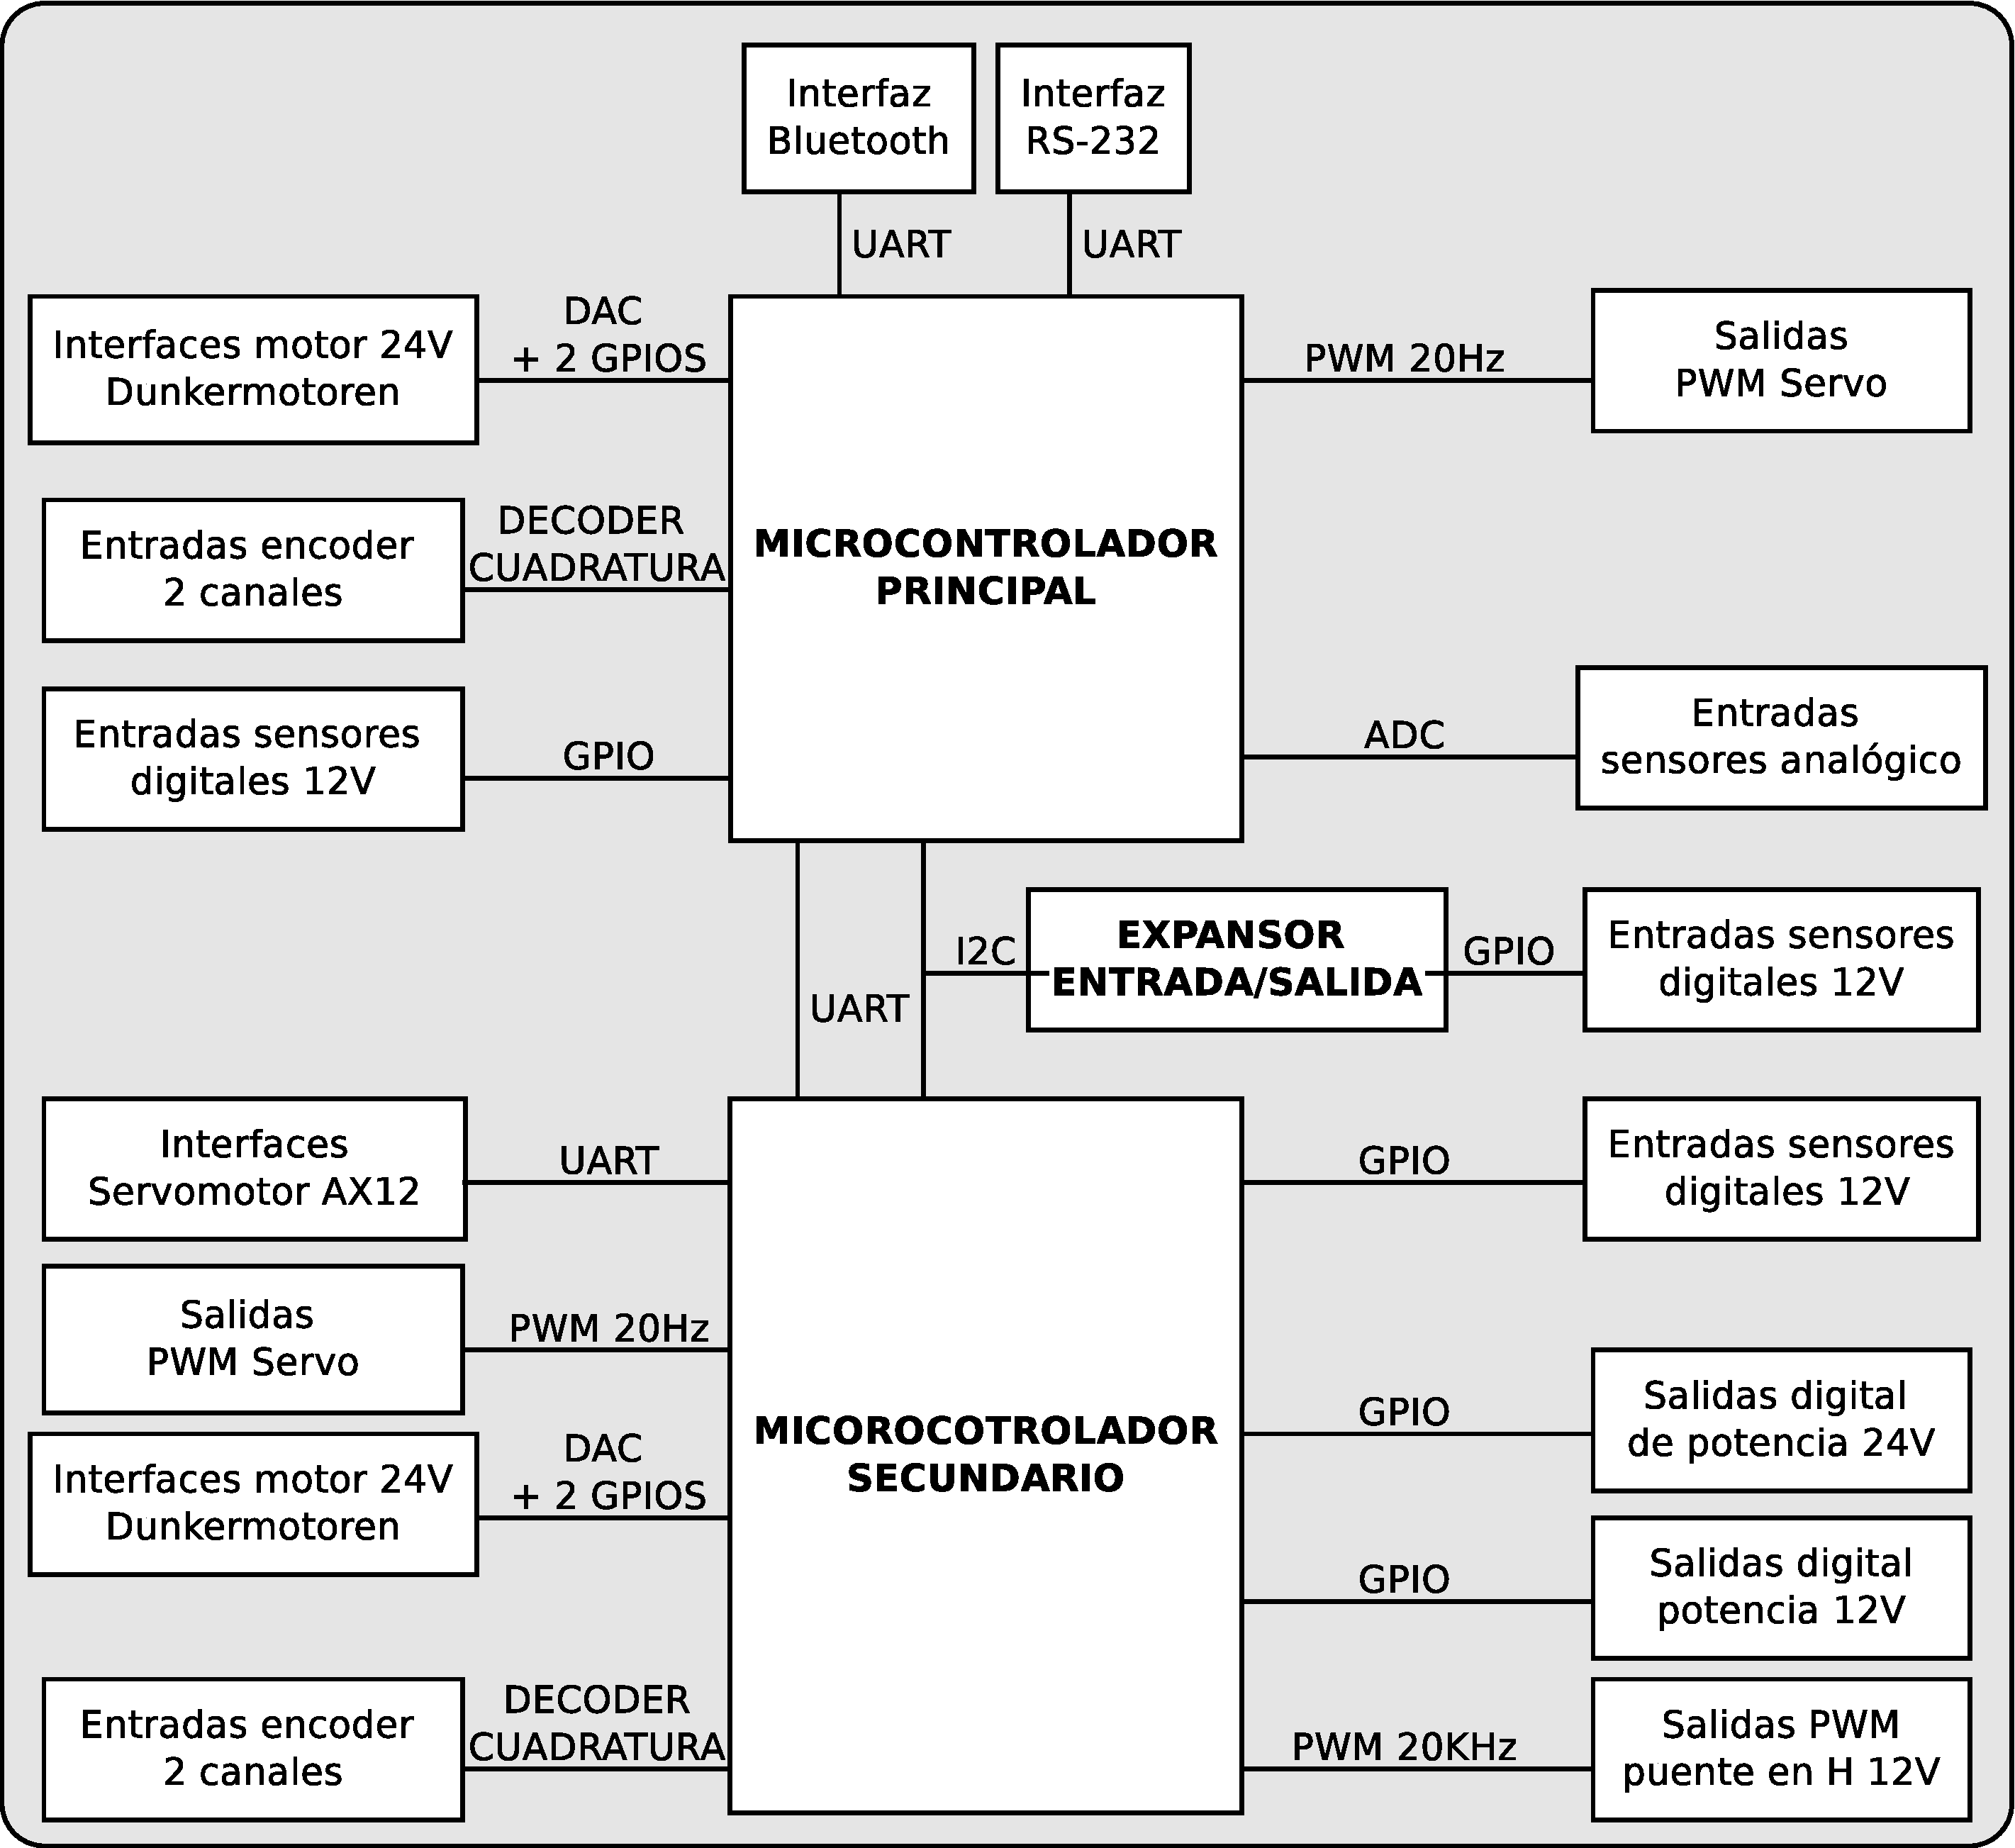
\includegraphics[width=.9\textwidth]{hardware_arquitectura_principal}
\caption[]{Arquitectura hardware desarrollada}
\label{fig_hardware_arquitectura_principal_resumen}
\end{figure}

Por otro lado, la arquitectura HW tiene una interfaz de depuraci�n RS-232 independiente a trav�s de la cual poder controlar, monitorizar y probar el hardware y el software. Esta interfaz forma una cadena serie con el resto de microcontroladores que permite acceder a cualquiera de ellos mediante un \emph{bypass} del los datos. Adem�s la arquitectura cuenta con una interfaz inal�mbrica Bluetooth mediante la cual se implementa la comunicaci�n con la baliza tipo faro y el robot secundario. El resto de recursos E/S de la arquitectura HW est�n pensados para la conexi�n de los actuadores y sensores m�s utilizados en el desarrollo de robots de Eurobot. Dependiendo de las caracter�sticas del robot, esta arquitectura HW ha sido implementada en diferentes tarjetas electr�nicas.

% SW

Al igual que la arquitectura HW, el software desarrollado est� basado en una \textbf{arquitectura software} pensada para se f�cilmente reutilizada y adaptada en cada desarrollo de un robot de Eurobot. El diagrama de bloques SW correspondiente a un robot principal y uno secundario se muestra en la figura \ref{fig_sw_diagrama_bloques_resumen}. Ambos robots implementan la misma arquitectura. El robot principal imlementa la arquitectura mediante dos microcontroladores y el secundario mediante un �nico microcontrolador.

\begin{figure}[ht]
\centering
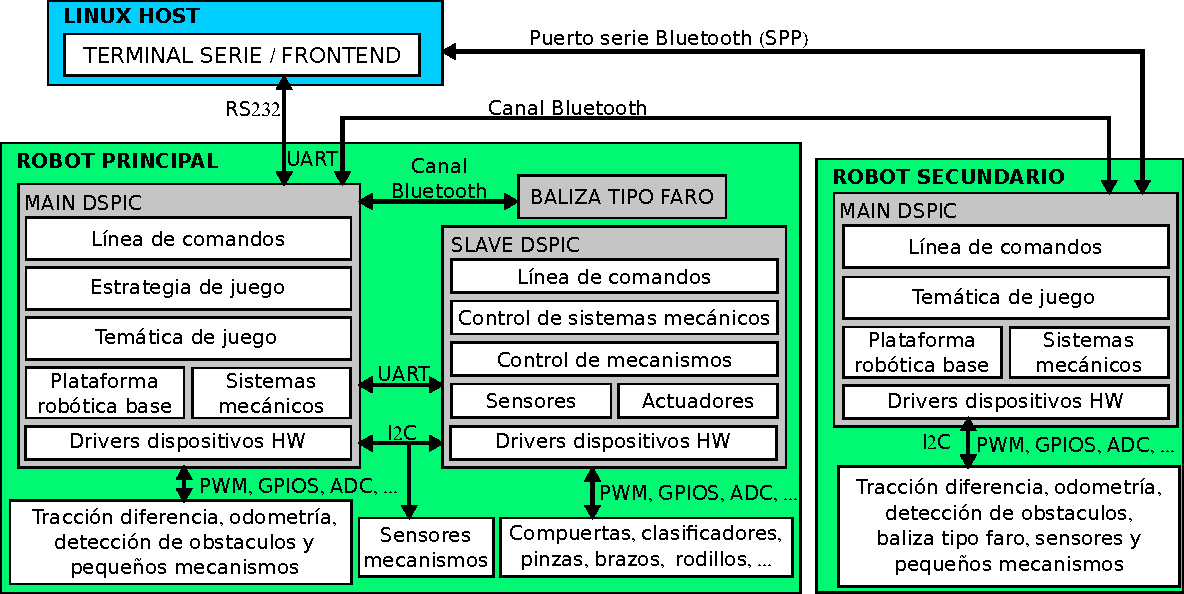
\includegraphics[width=\textwidth]{sw_diagrama_bloques}
\caption[]{Diagrama de bloques software del robot principal y secundario}
\label{fig_sw_diagrama_bloques_resumen}
\end{figure}

La arquitectura SW se organiza en capas o m�dulos funcionales, de forma que aquellos de nivel superior implementan funciones m�s abstractas que los inferiores:

\begin{description}
\item \textbf{Drivers de dispositivos HW}

Capa de menor nivel que permite abstraer los m�dulos o dispositivos HW del robot, como m�dulos de comunicaci�n del microcontrolador (UART, I2C, SPI, ...) o dispositivos externos a �ste como servomotores, o drivers en puente en H para el control de motores.

\item \textbf{Plataforma rob�tica base}

M�dulo que implementa las funcionalidades de la plataforma rob�tica base: control de posici�n, odometr�a, gesti�n de trayectorias y evitaci�n de obst�culos.

\item \textbf{Sistemas mec�nicos}

M�dulo que abstrae el control de los diferentes sistemas mec�nicos del robot mediante los cuales se manipulan los elementos del  juego. Este m�dulo a su vez se encuentra dividido en varios niveles, representados en el microcontrolador esclavo del robot principal de la figura \ref{fig_sw_diagrama_bloques_resumen}).

\item \textbf{Tem�tica de juego}

Nivel que integra toda la funcionalidad de los niveles inferiores y sistemas externos, como la baliza y el robot secundario, para implementar las funcionalidades del robot relativas a la prueba de Eurobot y a la navegaci�n del robot por el campo de juego.

\item \textbf{Estrategia de juego}

Esta capa implementa la estrategia de juego de un partido as� como las diferentes fases de las que se compone un partido.

\item \textbf{Linea de comandos}

Capa de mayor nivel que permite ejecutar comandos de cualquier m�dulo o nivel. De esta forma durante el desarrollo de las diferentes capas o m�dulos, las funcionalidades de �stas pueden ser probadas por partes y verificar su correcto funcionamiento.

\end{description}
 
Por �ltimo, el SW desarrollado incluye adamas un \textbf{simulador de los robots y del campo de juego}, implementado a partir la compilaci�n del c�digo fuente de los robots en un \emph{host} GNU/Linux.






%%% Local Variables:
%%% TeX-master: "../book"
%%% End:


       % EDIT this file

% Now include toc and list of figures+tables
\input{cover/toc+lof+lot.tex}                 % DO NOT TOUCH THIS LINE!

% If you want to include additional listings, you can use the float
% package. As an example, I include here the listing of source code
% snippets (you have some examples in appendix/manual.tex)
%\input{cover/extralistings.tex}               % Edit this file or
                                              % comment it out

% Now include acronyms (if this is the case)
%\input{acronyms/acronymsgl.tex}               % EDIT this file or
                                              % comment it out if you do
                                              % not use acronyms

% Now include symbols (if this is the case)
%\input{symbols/symbolsgl.tex}                 % EDIT this file or
                                              % comment it out if you do
                                              % not use acronyms

%
% END within-document configuration, frontpage and cover pages generation
%%%%%%%%%%%%%%%%%%%%%%%%%%%%%%%%%%%%%%%%%%%%%%%%%%%%%%%%%%%%%%%%%%%%%%%%%%%


%%%%%%%%%%%%%%%%%%%%%%%%%%%%%%%%%%%%%%%%%%%%%%%%%%%%%%%%%%%%%%%%%%%%%%%%%%%
% Now start text and numbering for mainmatter (chapter+appendices)
%%%%%%%%%%%%%%%%%%%%%%%%%%%%%%%%%%%%%%%%%%%%%%%%%%%%%%%%%%%%%%%%%%%%%%%%%%%
\mainmatter                                       % DO NOT TOUCH THIS LINE!
\deactivatetilden                                 % DO NOT TOUCH THIS LINE!


%%%%%%%%%%%%%%%%%%%%%%%%%%%%%%%%%%%%%%%%%%%%%%%%%%%%%%%%%%%%%%%%%%%%%%%%%%%
%%%%%%%%%%%%%%%%%%%%%%%%%%%%%%%%%%%%%%%%%%%%%%%%%%%%%%%%%%%%%%%%%%%%%%%%%%%
%%%%%%%%%%%%%%%%%%%%%%%%%%%%%%%%%%%%%%%%%%%%%%%%%%%%%%%%%%%%%%%%%%%%%%%%%%%
%%%%%%%%%%%%%%%%%%%%%%%%%%%%%%%%%%%%%%%%%%%%%%%%%%%%%%%%%%%%%%%%%%%%%%%%%%%
%%%%%%%%%%%%%%%%%%%%%%%%%%%%%%%%%%%%%%%%%%%%%%%%%%%%%%%%%%%%%%%%%%%%%%%%%%%
%%%%%%%%%%%%%%%%%%%%%%%%%%%%%%%%%%%%%%%%%%%%%%%%%%%%%%%%%%%%%%%%%%%%%%%%%%%
%%%%%%%%%%%%%%%%%%%%%%%%%%%%%%%%%%%%%%%%%%%%%%%%%%%%%%%%%%%%%%%%%%%%%%%%%%%
% BEGIN Normal chapters. Edit/modify all within this section
%
% I don't recommend it, but if you want to define "parts", use this...
% BEWARE: I didn't write the english dependent code
%\part*{Memoria}
%\label{part:memoria}

%%%%%%%%%%%%%%%%%%%%%%%%%%%%%%%%%%%%%%%%%%%%%%%%%%%%%%%%%%%%%%%%%%%%%%%%%%%
%
% Generic template for TFC/TFM/TFG/Tesis
%
% $Id: introduccion.tex,v 1.6 2014/02/11 11:00:06 macias Exp $
%
% By:
%  + Javier Mac�as-Guarasa.
%    Departamento de Electr�nica
%    Universidad de Alcal�
%  + Roberto Barra-Chicote.
%    Departamento de Ingenier�a Electr�nica
%    Universidad Polit�cnica de Madrid
%
% Based on original sources by Roberto Barra, Manuel Oca�a, Jes�s Nuevo,
% Pedro Revenga, Fernando Herr�nz and Noelia Hern�ndez. Thanks a lot to
% all of them, and to the many anonymous contributors found (thanks to
% google) that provided help in setting all this up.
%
% See also the additionalContributors.txt file to check the name of
% additional contributors to this work.
%
% If you think you can add pieces of relevant/useful examples,
% improvements, please contact us at (macias@depeca.uah.es)
%
% Copyleft 2013
%
%%%%%%%%%%%%%%%%%%%%%%%%%%%%%%%%%%%%%%%%%%%%%%%%%%%%%%%%%%%%%%%%%%%%%%%%%%%

\chapter{Introducci�n al proyecto}
\label{cha_introduccion}

\begin{FraseCelebre}
  \begin{Frase}
Todo el mundo es capaz de hacer cosas extraordinarias, cada uno a su manera. Algunos son perfectamente felices haciendo cosas simples de buen humor; otros, sin embargo, se concentran en los detalles. Somos todos diferentes, y no importa realmente si te centras en viajes espaciales o trabajas en el campo. Lo que importa es hacer lo que verdaderamente quieres.
  \end{Frase}
  \begin{Fuente}
    Alexander Kemurdzhian
  \end{Fuente}
\end{FraseCelebre}


\section{Presentaci�n}
\label{sec_presentacion}

Este trabajo de fin de carrera trata sobre el desarrollo de robots para la competici�n de robots Eurobot \cite{eurobot}. Pretende ser un manual de referencia para todo aquel que quiera construir un robot para participar en Eurobot\footnote{O para desarrollar un robot de similares caracter�sticas para cualquier otro cometido}. Todo lo que se expone en este libro se sustenta en la experiencia adquirida en el desarrollo de robots participantes en Eurobot entre los a�os 2003 y 2015. Especialmente en el periodo entre 2010 y 2015.

\section{La competici�n Eurobot}
\label{sec_la_competicion_eurobot}

Eurobot es un concurso internacional de rob�tica creado en 1998 a partir de la Copa de Francia de la rob�tica \cite{cdr} (Coupe de France de robotique). El concurso est� abierto a equipos de j�venes, organizados ya sea en proyectos de estudiantes o en clubes independientes. Eurobot se lleva a cabo en Europa, pero da la bienvenida a los equipos de todos los continentes.

Cada a�o, las reglas se publican alrededor de octubre. Los equipos tienen entonces varios meses para dise�ar y construir sus robots y competir entre abril y junio en el concurso nacional, en el cual se pueden seleccionar s�lo 3 equipos por pa�s. Los mejores equipos de cada pa�s se reunir�n despu�s para competir en las finales de Eurobot.

Las reglas cambian cada a�o, sin embargo, la base es siempre la misma:

\begin{itemize}
\item Los robots tienen aproximadamente el tama�o de un cubo de 30 cm.
\item El campo de juego tiene una dimensi�n de 2 metros de ancho y 3 metros de largo.
\item El juego tiene 90 segundos de duraci�n.
\item Los robots tienen que llevar a cabo varias tareas en el campo con el fin de ganar tantos puntos como sea posible.
\item Los robots tienen que evitarse unos a otros y evitar los choques.
\item Los robots son completamente aut�nomos y deben hacer todas las acciones por ellos mismos.
\end{itemize}

Tal y como est� dise�ado, Eurobot constituye un reto de ingenier�a que permite a alumnos de electr�nica, mec�nica e inform�tica aplicar sus conocimientos o ampliarlos y compartirlos. Tambi�n hace, por ejemplo, que alumnos de electr�nica aprendan mec�nica y/o inform�tica. Dada la complejidad de los robots suelen ser construidos por equipo formados de al menos 2 personas, lo cual implica cierta organizaci�n, divisi�n de tareas y trabajo en equipo. Un equipo numeroso permite desarrollar robots con partes m�s especializadas pero implica una gesti�n y coordinaci�n mayor. Por otro lado, Eurobot implica confeccionar un producto completo, original y funcional desde cero\footnote{No siempre se ha de empezar desde cero, un desarrollo modular y estructurado permite partir de una base m�nima.} (o como dir�amos en Ingl�s \emph{from scratch}) en cosa de 6 o 7 meses. Esto implica una elecci�n y compra de materiales, componentes, dise�o electr�nico y mec�nico, construcci�n de prototipos, desarrollo de software, ... y en definitiva una gesti�n del tiempo. Tiempo que suele escasear porque los participantes, generalmente alumnos, disponen de �l escasamente\footnote{Y parece ser que menos a�n con los actuales planes de estudios Bolonia}.


La comunidad de Eurobot se comunica principalmente a trav�s de sus foros \cite{foros_eurobot}. Hay tres foros principales: un foro relacionado con las reglas de cada a�o, el foro de Eurobot Open \cite{foro_eurobot_open} y el foro de la Copa de Francia de la rob�tica \cite{foro_copa_francia}. Este �ltimo es el foro m�s activo dado que la Copa nacional de Francia es la de mayor tradici�n y la que re�ne el mayor numero de participantes. Este foro, aunque est� escrito en franc�s, es el que acumula la mayor�a de la informaci�n acerca de la competici�n y de temas t�cnicos. Adem�s, cada equipo suele tener una p�gina web, blog o canal de Youtube donde comparte los avances de los robots que construyen cada a�o.

Eurobot est� organizada gracias la asociaci�n internacional de Eurobot y a la asociaci�n francesa \emph{Planet Sciences} \cite{planet_sciences} y a muchas otras asociaciones, escuelas, universidades y personas voluntarias de los pa�ses participantes. Es incre�ble la cantidad de personas que apoyan Eurobot y trabajan de forma voluntaria sin ninguna remuneraci�n m�s que la satisfacci�n de estar implicados y formar parte de esta fiesta que es Eurobot. Y esto incluye a los participantes, ya que ganar Eurobot no implica ning�n premio econ�mico. En total, un mont�n de gente que trabaja para disfrutar y divertirse con la rob�tica.

\section{El equipo \emph{Eurobotics Engineering}, historia y antecedentes}
\label{sec_equipo_eurobotics}

\emph{Eurobotics Engineering} \cite{arc_robots} es un equipo participante en Eurobot formado por entusiastas de la rob�tica. Est� formado por estudiantes de la Universidad de Alcal� (UAH): ingenieros de telecomunicaci�n, de electr�nica, de telem�tica y de electr�nica industrial.

La historia de este equipo se remonta al a�o 2003, a�o en el que el Departamento de Electr�nica de la UAH decide montar un equipo patrocinado a partir de la iniciativa de un grupo de alumnos de participar en Eurobot 2002. Los integrantes del equipo se renuevan cada a�o excepto algunos que se mantienen. Exceptuando el a�o 2009, el resto de a�os el equipo particip� en Eurobot. En el a�o 2010 Diego Salazar y Javier Bali�as crean el equipo de Eurobot llamado \emph{Eurobotics Engineering} y en el a�o 2011, junto con Nilo Masias, fundaron la Asociaci�n de Rob�tica de Coslada (ARC).

El equipo Eurobot Engineering particip� en Eurobot desde el a�o 2010 hasta el a�o 2015 (exceptuando el a�o 2013). Durante estos a�os ha contado con el apoyo del Dpto. de Electr�nica de la Universidad de la UAH \cite{depeca,uah} y el Ayuntamiento de Coslada, adem�s del patrocinio de Ayudas Hidr�ulicas \cite{ayudas_hidraulicas}, Carpinter�a Ingl�s, Ro-botica \cite{ro_botica} (2010-2012), el Consejo de estudiantes de la UAH \cite{consejo_de_estudiantes} (2014-2015) y Mobile Minds \cite{mobile_minds} (2015).

La siguiente tabla muestra un resumen de los robots desarrollados para la competici�n Eurobot desde el a�o 2003 hasta el a�o 2015, en los que ha participado el autor del libro junto con otras personas implicadas en su desarrollo.

\begin{center}
	\begin{longtable}{|c|c|c|p{5cm}|}
    \caption{Robots desarrollados para la competici�n Eurobot (2003-2015).} \label{tab_robots_desarrollados} \\
    
    \hline 
	\multicolumn{1}{|c|}{\textbf{A�o}} & 
	\multicolumn{1}{c|}{\textbf{Prueba}} & 
	\multicolumn{1}{c|}{\textbf{Robots}} & 
	\multicolumn{1}{p{5cm}|}{\textbf{Integrantes equipo}} \\ 
	\hline 
    \endfirsthead
    
    \multicolumn{4}{c}%
    {{\bfseries \tablename\ \thetable{} -- contin�a en la p�gina anterior}} \\
    \hline 
	\multicolumn{1}{|c|}{\textbf{A�o}} & 
	\multicolumn{1}{c|}{\textbf{Prueba}} & 
	\multicolumn{1}{c|}{\textbf{Robots}} & 
	\multicolumn{1}{p{5cm}|}{\textbf{Integrantes equipo}} \\ 
	\hline 
    \endhead
    
    \hline \multicolumn{4}{|r|}{{Contin�a en la p�gina siguiente}} \\ \hline
    \endfoot

    \hline \hline
    \endlastfoot
    
%   \hline	
%	% a�o, prueba, robot
%	2002 &	Flying Billiards &	Ligre &	
%	% equipo e integrantes	 
%	\textbf{Depeca UAH:} \newline
%	Santiago Cobreces Alvarez \newline
%	Miguel Garc�a P�rez \newline
%	Pedro Jimenez Molina \newline
%	Fernando M�ndez Rebollo \newline
%	Jesus Nuevo Chiquero \newline
%	Dam Peinador Aranda \newline
%	Daniel Pizarro Perez \\

    \hline	
	% a�o, prueba, robot
	2003 &	Heads or Tails & Husillo &
	% integrantes
	Julio Pastor \newline
	Juan Carlos Garc�a \newline
	Diego Alonso Garc�a \newline
	Enrique Moraleja Garc�a \newline
	Jose Manuel G�mez Sanchez	\newline
	Alberto Sanchez Rodr�guez \newline
	Gustavo Tapias \newline
	Javier Peletier \newline
	Jes�s Oliva \newline
	Santiago Cobreces Alvarez \newline
	Daniel Pizarro Perez \newline
	Pedro Yag�e \newline
	Pedro Jim�nez \newline
	Mario Ingl�s Garc�s \newline
	Javier Bali�as Santos \\

    \hline	
	% a�o, prueba, robot
	2004 &	Coconut Rugby &	Electrococo y Joselito	&
	% integrantes
	Julio Pastor \newline
	Oscar G�nz�lez \newline
	Santiago Cobreces \newline
	Diego Alonso Garc�a \newline
	Enrique Moraleja Garc�a \newline
	Jose Manuel G�mez Sanchez	\newline
	Ra�l Sanchez de la Monta�a \newline
	Javier Antunez \newline
	Santiago Castillo \newline
	Saleta Nistal \newline
	Javier Rodriguez \newline
	David Mollejo \newline
	Noelia Requena \newline
 	Till Zenthoefer \newline
	Cesar Guerra \newline
	Cesar Lozano \newline
	Jordi Polo \newline
	Jorge Fernandez \newline
	Mario Ingl�s Garc�s \newline
	Javier Bali�as Santos \\

    \hline	
	% a�o, prueba, robot
	2005 & Bowling & Campanolo &
	% integrantes
	Julio Pastor \newline
	Mario Ingl�s Garc�s \newline
	Javier Bali�as Santos \\

%    \hline	
	% a�o, prueba, robot
%	2006 & Golf & - & 
%	Caponata &
	% integrantes
%	Sergio Arroyo Sierra \newline
%	Marcelo Salazar Acucci 
%	- \\

    \hline	
	% a�o, prueba, robot
	2007 & Recycling & Mr. Proper &
	% integrantes
	Julio Pastor \newline
	Sergio Arroyo Sierra \newline
	Marcelo Salazar Acucci \newline
	Diego Salazar Acucci \newline
	Adrian D�az Collazo \newline
	Rub�n Arcos Moreno \newline
	Mario Ingl�s Garc�s \newline
	Javier Bali�as Santos \\

    \hline	
	% a�o, prueba, robot
	2008 &	Mission to Mars & Topolino &
	% integrantes
	Sergio Arroyo Sierra \newline
	Marcelo Salazar Acucci \newline
	Diego Salazar Acucci \newline
	Mario Ingl�s Garc�s \newline
	Javier Bali�as Santos \\

%    \hline	
	% a�o, prueba, robot
%	2009 &	Temples of Atlantis & - &
	% integrantes
%	- \\

    \hline	
	% a�o, prueba, robot
	2010 &	Feed the world & Trompetero &
	% integrantes
	Mario Ingl�s Garc�s \newline
	Diego Salazar Acucci \newline		 
	Javier Bali�as Santos \\		 

    \hline	
	% a�o, prueba, robot
	2011 & Chess'Up! & Zamorano &
	% integrantes
	Nilo Masias Carranza \newline	
	Mario Ingl�s Garc�s \newline
	Diego Salazar Acucci \newline		 
	Javier Bali�as Santos \\		 

    \hline	
	% a�o, prueba, robot
	2012 & Treasure island & Crisp�n y Autom�tico &
	% integrantes
	Sergio Arroyo Sierra \newline
	Nilo Masias Carranza \newline
	Mario Ingl�s Garc�s \newline
	Diego Salazar Acucci \newline		 
	Silvia Santano Guill�n \newline
	Javier Bali�as Santos \\		 

    \hline	
	% a�o, prueba, robot
	2013 & Happy birthday &	- &
	% integrantes
	- \\

    \hline	
	% a�o, prueba, robot
	2014 & Prehistobot & Grosnik y Sesk�pa &
	% integrantes
	Mario Ingl�s Garc�s \newline
	Diego Salazar Acucci \newline		 
	Silvia Santano Guill�n \newline
	Javier Rodriguez Puigvert \newline
	Miguel Ortiz \newline
	Carlos de la Rubia \newline
	Rub�n Espino San Jos� \newline
	Javier Bali�as Santos \\		 

    \hline	
	% a�o, prueba, robot
	2015 & Robomovies & P.Tinto y Tirantes &
	% integrantes
	Mario Ingl�s Garc�s \newline
	Silvia Santano Guill�n \newline
	Javier Rodriguez Puigvert \newline
	Carlos de la Rubia \newline
	Rub�n Espino San Jos� \newline
	Javier Bali�as Santos \\
	\end{longtable}
\end{center}


	

\section{La rob�tica educativa}
\label{sec_robotica_educativa}

A d�a de hoy la rob�tica constituye una herramienta educativa muy potente. Permite aprender y poner en practica diferentes ramas de la ciencia. Lo hace a trav�s de la ingenier�a y las �reas de la ciencia en las que se sustenta (matem�ticas, f�sica, qu�mica, entre otras) y utilizando la tecnolog�a actual. Este tipo de educaci�n se denomina STEM \cite{stem} acr�nimo del ingl�s \emph{Science, Technology, Engineering and Mathematics} (Ciencia, Tecnolog�a, Ingenier�a y Matem�ticas). Adem�s permite potenciar la creatividad de las tecnolog�as digitales, m�s all� de la simple explotaci�n de ellas \cite{strategy_1_0}.

Adem�s si la rob�tica se hace en equipo, como suele ser habitual en Eurobot, la rob�tica permite desarrollar habilidades y competencias \cite{robocompetences} como el trabajo en grupo, la motivaci�n personal, gesti�n de retos y objetivo, y el manejo del fracaso y las emociones que implican los errores, entre otras.

Este trabajo de fin de carrera constituye en s� un ejemplo de la rob�tica como herramienta educativa y de sus resultados. Los robots desarrollados ha ayudado adquirir experiencia, conocimientos y experiencias de gran valor a�adido a los estudios universitarios de los diferentes integrantes del equipo \emph{Eurobotics Engineering} y anteriores.

En el campo de la ingenier�a electr�nica y mec�nica, se ha ganado experiencia en el proceso de dise�o, fabricaci�n y montaje de productos que implican una electr�nica y una mec�nica (tarjetas electr�nicas, piezas mec�nicas, mecanismos, cableado, etc). Se han aprendido a trabajar con diferentes tipos de materiales (madera, pl�stico, aluminio, pol�meros, etc), a utilizar herramientas y a fabricar piezas mec�nicas por diferentes procesos de fabricaci�n (impresi�n 3D, fresado, plegado, inyecci�n en silicona, etc.).

El simple hecho de que los robots se muevan y que lo hagan hacia lugares concretos implica la aplicaci�n de las matem�ticas y la f�sica. As�, para ir de un punto $A$ a un punto $B$ se utiliza la trigonometr�a. Esto es, el robot necesita mirar a $B$ (girar un �ngulo $\alpha$) y luego avanzar una distancia $d$. Y adem�s si se desea el tiempo en ir de $A$ a $B$ sea el menor posible es necesario utilizar las leyes de Newton para el calculo de la aceleraci�n y velocidad m�xima, que permitan al robot no derrapar ni pasarse de frenada.

Especialmente, dado que un robot en �ltima medida es controlado desde un microcontrolador o procesador similar, la rob�tica implica adquirir conocimientos sobre la ingenier�a del software y el desarrollo de sistemas embebidos\cite{making_embedded_systems}. Seguramente alg�n momento se quiera utilizar una librer�a o c�digo desarrollada por otras personas pero que resulta muy �til. Se tendr� que aprender a manejar y confiar en librer�as de terceros y si son de c�digo abierto quiz� permita colaborar a�adiendo nuevas funcionalidades o solucionar bugs. Se aprende mucho analizando y comprendiendo el c�digo de otros. Adem�s seguramente estas librer�as utilizar�n alg�n sistema de control de versiones distribuido como Git, Mercurial o centralizado como SVN o incluso sistemas m�s antiguos como CVS. La mayor�a de los desarrolladores de software son reacios al principio a utilizar un sistema de control de versiones, suele ser una decisi�n personal que normalmente cae por su propio peso cuando se trabaja con proyectos de c�digo extensos.

A medida que el c�digo desarrollado vaya creciendo surgen planteamientos de como organizarlo, c�mo reutilizar c�digo de un a�o a otro o incluso c�mo reutilizar c�digo del microcontrolador que se est� utilizando para poder utilizarlo en otros proyectos. Esto lleva a desarrollar c�digo de una forma m�s modular y estratificada. Quiz� m�s adelante, el microcontrolador utilizado hasta el momento se quede escaso de recursos, se quiera cambiar a otro de la misma familia pero con m�s recursos y reutilizar las librer�as que se han desarrollado hasta entonces y mantener la compatibilidad con el antiguo microcontrolador. Esto por ejemplo se puede lograr mediante la compilaci�n condicional.

Al ir ganando experiencia, se es capaz de detectar las partes fundamentales y comunes a la hora de implementar una aplicaci�n o funcionalidad. Si se observa como lo ha resuelto el resto del mundo se cae en la cuenta que hay ciertas cosas que ya est�n muy estudiadas y aparecen en cualquier aplicaci�n que desarrollemos. As� se podr� detectar y aplicar patrones que facilitan desarrollo.

Quiz� llegue un momento en que el tiempo que lleva realizar la depuraci�n del robot sobre el entorno real es mucho y es un proceso lento, o quiz� no se disponga de dicho entorno porque no queda otra opci�n que desarrollar de forma remota. Para todo eso, es muy �til el uso de simuladores o bancos de pruebas\footnote{Tambi�n conocidos en la literatura anglosajona como \emph{sandbox}.} que permiten emular las interfaces de entrada y salida del robot (sensores y motores) o sus est�mulos (obst�culos).

La rob�tica se disfruta, es divertida, pero tambi�n se sufre y requiere de un indudable ejercicio de abstracci�n y concentraci�n. Es necesario investigar sobre cosas nueva o reforzar conocimientos ya adquiridos, aplicarlos y madurarlos. Son m�s comunes los errores que los aciertos, nada sale a la primera, y la \emph{ley de Murphy}\footnote{"Si algo puede salir mal, saldr� mal"} suele no fallar.  Todo esto lleva al aprendizaje y aplicaci�n del \emph{m�todo cient�fico} para experimentar o para resolver problemas encontrados, como comportamientos no esperados del robot.

Durante el desarrollo de la rob�tica, puede parecer que es una actividad poco agradecida o agradecida en momentos muy cortos. Pero merece la pena y adem�s se demuestra que m�s tarde, en el mundo laboral o de la investigaci�n, es cuando la rob�tica tiene gran parte su retorno\footnote{El autor de este proyecto esta convencido de ello y lo ha experimentado.}.


\section{Aprendiendo de gigantes.}
\label{sec_aprendiendo_de_gigantes}

Hoy en d�a es casi impensable que una sola persona pueda realizar avances en los diferentes campos de la ciencia equiparables a los descubrimientos de los grandes cient�ficos de la historia. As� la investigaci�n y el desarrollo tecnol�gico son llevados a cabo por grupos de personas cada cual experta en ciertos tema concretos. Por otro lado la tecnolog�a y sus aplicaciones cada vez son m�s complejas y eso es en gran parte a que los nuevos desarrollos se apoyan en desarrollos anteriores que permiten abstraerse de aquello que se encuentra fuera del alcance de un objetivo concreto.

Quiz� el ejemplo m�s conocido a d�a de hoy es la plataforma de desarrollo Arduino \cite{arduino} que permite desarrollar sistemas embebidos partiendo de un conocimiento muy b�sico o nulo sobre microcontroladores. Esto es gracias a que la plataforma de desarrollo Arduino tiene una vasta librer�a de funciones que abstraen la programaci�n de bajo nivel del microcontrolador de forma que no se \emph{escribe un bit} de uno o varios \emph{registros} de nombres aparentemente sin significado, si no que se \emph{detiene}, se \emph{cambia el sentido} o se \emph{cambia la velocidad} de un \emph{motor}. Adem�s todas esas funciones se encuentran documentadas y son accesibles \cite{arduino_src} para su modificaci�n o consulta. As�, si una funcionalidad de una librer�a no existe, es posible estudiar como est� implementada y a�adir nuevas funcionalidades.

En cierta forma, esta manera de abordar el aprendizaje y el desarrollo de aplicaciones tecnol�gicas es una forma natural y acorde con el desarrollo tecnol�gico de la sociedad actual. Hoy en d�a la tecnolog�a que utilizamos en el d�a a d�a es compleja y muy abstracta por lo que no tiene sentido que el aprendizaje de la misma comience desde los niveles m�s b�sicos. Plataformas como Arduino permiten comenzar en un punto intermedio y poder crecer hacia niveles de abstracci�n mayores (grano grueso) o hacia niveles inferiores m�s espec�ficos (grano fino).

Pues bien este proyecto no es una excepci�n y tambi�n se ha apoyado en hombros de gigantes. El c�digo fuente de los microcontroladores de algunos de los robots desarrollados (Husillo, Joselito o Campanolo) fue escrito desde cero. Otros (Electrococo, Mr.Proper y Topolino) se ayudaron del c�digo escrito en a�os anteriores para otros robots. Y finalmente a partir del a�o 2010 los robots (Trompetero, Zamorano, Crisp�n, Autom�tico, Grosnik, Sesk�pa, P.Tinto y Tirantes) se desarrollaron a partir del c�digo abierto escrito por terceros.

El utilizar c�digo abierto de terceros vino dado por el objetivo de evolucionar tecnol�gicamente los robots a desarrollar para Eurobot. Para ello se estudi� los fundamentos t�cnicos y tecnol�gicos de los robots por aquella �poca obten�an muy buenos resultados como RCVA \cite{rcva}, Microb Tecnology \cite{microb}, RCA Archen \cite{rca_aachen} o Turak \cite{turak}. Al final de dicho estudio se establecieron los requisitos de la mec�nica, hardware y software necesarios, y se desarrollo una plataforma rob�tica base (el \emph{Dummy robot}, ver \ref{fig_dummy_robot}) con una mec�nica y una electr�nica de acuerdo a los requisitos buscados.

\begin{figure}[h]
\centerline{
	\subfloat[Dise�o 3D]{\includegraphics[height=.2\textheight]{dummy_robot_1}
	\label{fig_dummy_robot_3d}}
	\hfil
	\subfloat[Prototipo mec�nico]{\includegraphics[height=.2\textheight]{dummy_robot_2}
	\label{fig_dummy_robot_prototipo}}
}
\centerline{
	\subfloat[Tarjeta electronica dsPIC33]{\includegraphics[height=.2\textheight]{dummy_robot_tarjeta_dspic33}
	\label{fig_dummy_robot_tarjeta_dspic33}}
}

\caption[Plataforma rob�tica \emph{Dummy robot}]{\emph{Dummy robot}. Plataforma rob�tica base desarrollada en 2010 por el equipo Eurobotics Engineering. Dise�o 3D, prototipo mec�nico y electr�nica basada en microcontrolador dsPIC33.}
\label{fig_dummy_robot}
\end{figure}



Al final del proceso de estudio se descubrieron las librer�as Aversive desarrolladas por el equipo \emph{Microb Technology} para microcontroladores AVR de Atmel. Por aqu�l entonces, la electr�nica que se estaba dise�ando estaba basada en microcontrolador dsPIC de Microchip. Se podr�a haber migrado el HW y utilizar microcontroladores AVR, pero al final se opt� por migrar las librer�as Aversive a la arquitectura de dsPIC, lo que se denomin� Aversive4dsPIC\footnote{Pronunciado \emph{Aversive for dsPIC}, Aversive para dsPIC}.

La decisi�n de utilizar estas librer�as y portarlas permiti� no solo aprender a utilizarlas desde la capa de aplicaci�n (el robot) sino estudiar c�mo estaban implementadas y adaptarlas para ser compatibles con una arquitectura diferente. En definitiva se reutiliz� el c�digo de terceros, lo cual implica mucho m�s que el simple hecho de aprovechar el trabajo realizado por otros. En este caso las librer�as Aversive \cite{aversive_src} son unas librer�as libres desarrolladas por varias personas, versionada bajo un sistemas de control de versiones, que est�n muy bien estructuradas, escritas siguiendo una gu�a de estilo com�n, que explota al m�ximo el lenguaje ANSI C, que cuenta con un \emph{toolchain}\footnote{Cadena de herramientas: conjunto de programas mediante los cuales se construye el programa que se ejecuta en el microcontrolador} que utiliza herramientas libres, que implementan todo tipo de funcionalidades y muchas de ellas dirigidas al desarrollo de robots como los de Eurobot. La migraci�n de las librer�as Aversive se realiz� siguiendo y manteniendo toda las caracter�sticas anteriormente mencionada, lo cual implic� el aprendizaje de las mismas y de todos los conceptos derivados y subyacentes de ellas.     



\section{Motivaci�n y objetivos}
\label{sec_motivacion_y_objetivos}

Todo el trabajo realizado en el desarrollo de los diferentes robots viene principalmente motivado por la afici�n a la rob�tica, la electr�nica, los sistemas embebidos y por la inquietud de inventar y crear cosas.

Por otro lado, el objetivo fundamental de este trabajo es la divulgaci�n del conocimiento adquirido en la realizaci�n de robots que compiten en Eurobot, siendo los objetivos espec�ficos de este proyecto los siguientes:

\begin{itemize}
\item Reflexionar y analizar diferentes aspectos indirectamente relacionados con el desarrollo de ingenier�a (el equipo de trabajo, organizaci�n, ...)
\item Analizar y describir los fundamentos de ingenier�a impl�citos (din�mica, cinem�tica, sistemas de control, ...).
\item Describir las partes fundamentales del desarrollo (movimiento, navegaci�n, posicionamiento, estrategia ...) y dise�o un robot de Eurobot (mec�nica, electr�nica, programaci�n, ...).
\item Presentar implementaciones y dise�os reales de cada una de las partes fundamentales de un robot de Eurobot.
\item Documentar todas aquellos dise�os, desarrollos o algoritmos realizados que puedan servir de punto de partida o ser reutilizados en futuros desarrollos (dise�os electr�nicos, librer�as software, herramientas de simulaci�n, ...).
\end{itemize}

\section{Organizaci�n del libro}
\label{sec_organizacion_del_libro}

El libro cuenta con 5 cap�tulos adicionales a este cap�tulo:

\begin{description}

\item \textbf{El robot de Eurobot}

Cap�tulo que describe el robot de Eurobot desde el punto de vista de su desarrollo: las especificaciones funcionales, las partes principales de un robot de Eurobot, las caracter�sticas de la mec�nica, electr�nica y software, y las fases de su desarrollo.

%\item \textbf{El equipo de Eurobot:}

%Reflexi�n sobre el equipo de personas que desarrollan un robot de Eurobot y varios temas relacionados como el n�mero de integrantes, expectativas, motivaci�n y objetivos del equipo, divisi�n de tareas o la organizaci�n y metodolog�a de trabajo.

\item \textbf{Plataforma rob�tica base}

Descripci�n de lo que se ha considerado plataforma rob�tica base, un robot base cuyas caracter�sticas y funcionalidades son comunes a cualquier juego de Eurobot y sobre el que desarrollar nuevos robots participantes. El cap�tulo se centra en la plataforma rob�tica desarrollada de tracci�n diferencial y control de posici�n polar mediante odometr�a. Adem�s se describe el sistema desarrollado para la detecci�n y evitaci�n de los robots oponentes.

\item \textbf{Sistema de balizas tipo faro:}

Este cap�tulo se centra en la medida de la posici�n del robot oponente respecto al robot apoy�ndose en los soportes de balizamiento proporcionados por las reglas del juego. Se presenta uno de los sistemas m�s utilizados en Eurobot basado en una baliza tipo faro. El cap�tulo describe los fundamentos de este tipo de sistema y presenta el desarrollo de dos balizas tipo faro de implementaci�n mec�nica diferente pero que comparten una misma arquitectura hardware y un mismo software.

\item \textbf{Desarrollo hardware}

Se presenta la arquitectura hardware a partir de la cual se han desarrollado los diferentes robots desde el a�o 2010. Se describe c�mo la arquitectura fue dise�ada y pensada para poder ser reutilizada en cada desarrollo de un robot. Tambi�n se describen las diferentes implementaciones realizadas de la arquitectura en diferentes tarjetas electr�nicas en funci�n de las necesidades de cada tipo de robot desarrollado.

\item \textbf{Desarrollo software}

El cap�tulo sobe la arquitectura software implementada en los robots desarrollados. Se describe la organizaci�n y funcionamiento de los niveles o capas de los que se compone la implementaci�n SW del robot. 

%\item \textbf{Presupuesto}

%Cap�tulo que presenta el presupuesto correspondiente al desarrollo de uno de los �ltimos robots desarrollados, el robot P.Tinto. El cual fue desarrollado para competir en la prueba \emph{Robomovies} de Eurobot 2015. 

%\item \textbf{Sistemas mec�nicos para la manipulaci�n de elementos de juego:}

%Cap�tulo que trata sobre los sistemas mec�nicos (brazos, pinzas, catapultas, etc.) que se desarrollan espec�ficamente para manipular los elementos de juego de la prueba de Eurobot. Se realiza una revisi�n de las soluciones mec�nicas conocidas y utilizadas hasta la fecha por diferentes equipos. Y posteriormente se tratan los componentes fundamentales de estos sistemas mec�nicos (actuadores y sensores) y la forma de controlarlos y sincronizarlos con el movimiento del robot.  

%\item \textbf{Implementaci�n de la estrategia de juego:}

%Por �ltimo se trata el tema de la estrategia de juego de un robot de Eurobot. Se analiza los elementos y diferentes fases en las que se puede dividir un partido y los diferentes patrones de implementaci�n software. Se trata la gesti�n de trayectorias durante un partido, algo nada determinista dado que se compite con un oponente del que se desconoce el comportamiento. Adem�s tambi�n se habla de las estrategias con dos robots y sobre la simulaci�n de las estrategias y sus ventajas. 

\end{description}



%%% Local Variables:
%%% TeX-master: "../book"
%%% End:

%%%%%%%%%%%%%%%%%%%%%%%%%%%%%%%%%%%%%%%%%%%%%%%%%%%%%%%%%%%%%%%%%%%%%%%%%%%
%
% Generic template for TFC/TFM/TFG/Tesis
%
% $Id: introduccion.tex,v 1.6 2014/02/11 11:00:06 macias Exp $
%
% By:
%  + Javier Mac�as-Guarasa.
%    Departamento de Electr�nica
%    Universidad de Alcal�
%  + Roberto Barra-Chicote.
%    Departamento de Ingenier�a Electr�nica
%    Universidad Polit�cnica de Madrid
%
% Based on original sources by Roberto Barra, Manuel Oca�a, Jes�s Nuevo,
% Pedro Revenga, Fernando Herr�nz and Noelia Hern�ndez. Thanks a lot to
% all of them, and to the many anonymous contributors found (thanks to
% google) that provided help in setting all this up.
%
% See also the additionalContributors.txt file to check the name of
% additional contributors to this work.
%
% If you think you can add pieces of relevant/useful examples,
% improvements, please contact us at (macias@depeca.uah.es)
%
% Copyleft 2013
%
%%%%%%%%%%%%%%%%%%%%%%%%%%%%%%%%%%%%%%%%%%%%%%%%%%%%%%%%%%%%%%%%%%%%%%%%%%%

\chapter{El robot de Eurobot}
\label{cha_el_robot_de_eurobot}

\begin{FraseCelebre}
  \begin{Frase}
Somos como enanos subidos a hombros de gigantes. Nuestra mirada puede abarcar m�s cosas y ver m�s lejos que ellos. No porque nuestra vista sea m�s penetrante y nuestra estatura mayor sino porque nos ha elevado su altura gigantesca.
  \end{Frase}
  \begin{Fuente}
Bernardo de Chatres, en \emph{Metalogicon} de Juan de Salisbury
  \end{Fuente}
\end{FraseCelebre}



%\section{Introducci�n}

Cada robot que participa en Eurobot es �nico y diferente al resto, sin embargo todos tienen en com�n ciertas caracter�sticas o funcionalidades que vienen determinadas o derivadas de las reglas del juego. Como se ha comentado en el capitulo \ref{cha_introduccion} cada a�o la prueba en la que competir o a resolver es diferente, esto tiene una implicaci�n directa en el dise�o mec�nico especialmente en los mecanismos dise�ados para manipular los elementos de juego propios de la prueba. Sin embargo, si se comparan las reglas del juego de varios a�os se observan caracter�sticas comunes que repercuten en el dise�o de la mec�nica, de la electr�nica o del software.

\section{Especificaciones del robot de Eurobot}
\label{sec_especificaciones_del_robot_de_eurobot}

Un robot de Eurobot tiene especificaciones independientes de la tem�tica del juego y otras dependientes totalmente. Las primera permiten que una vez est�n desarrolladas y validadas puedan ser reutilizadas o mejoradas en futuros dise�os. Esto quiere decir que pueden ser un bloque totalmente modular, por ejemplo una tarjeta electr�nica, o dise�os reutilizables como el dise�o electr�nico de la tarjeta, cuyo PCB\footnote{Del ingl�s \emph{Printed Circuit Board}, Tarjeta de Circuito Impreso} puede dise�arse a medida del robot y en funci�n del espacio disponible.

Por otro lado, los sistemas mec�nicos a dise�ar para la manipulaci�n de los elementos de juego son en su mayor�a espec�ficos de cada prueba. S�lo una peque�a parte del desarrollo relacionado con estos sistemas es reutilizable, como es parte del desarrollo software destinado al control de dichos sistemas mec�nicos. 

Un robot de Eurobot ha de ser completamente aut�nomo y b�sicamente ser capaz de:

\begin{enumerate}
\item Desplazarse hasta las diferentes zonas del campo donde se sit�an los elementos del juego o donde se almacenan.
\item Evitar chocar con elementos del campo de juego y con otros robots oponentes durante los desplazamientos entre zonas del campo.
\end{enumerate}

Adem�s, si las reglas permiten dos robots por equipo: un robot principal y uno secundario, es recomendable que ambos robots sean capaces de comunicarse entre s� con el fin jugar de forma cooperativa.

Con el fin de facilitar la detecci�n entre los robots y que estos sean capaces de evitar colisiones entre ellos, los robots han de reservar un espacio para sensores y balizas a una altura determinada como muestra la figura \ref{fig_balizas_robots}. As�, cada robot puede colocar una baliza o marca en el robot oponente y disponer de un espacio donde situar los sensores apropiados para detectar dicha baliza. 

Estas balizas pueden ser activas o pasivas. Por ejemplo, un sistema compuesto por una baliza maciza y un sensor de ultrasonidos puede ser utilizado para detectar a qu� distancia y direcci�n se encuentra un robot oponente antes de tomar tomar la decisi�n de hacia donde redirigirse.

Adem�s el campo de juego cuenta con 3 soportes para balizas adicionales que est�n a disposici�n de cada equipo (ver figura \ref{fig_balizas_campo}). Estos soportes est�n pensados para facilitar la localizaci�n de los robots en el campo de juego. Por ejemplo, un sistema compuesto por una baliza reflectante colocada en el soporte de una esquina del campo y un sensor de luz reflexivo en el robot puede ser utilizado para localizar una canasta que se encuentre en dicha esquina del campo.

Las balizas pueden ser activas o pasivas y tiene como �nicas restricciones sus dimensiones y peso:

\begin{itemize}
\item Balizas colocadas en el oponente: dimensiones m�ximas de 80x80x80 cm y peso m�ximo de 0,5 Kg.
\item Balizas del campo de juego: dimensiones m�ximas de 160x80x80 cm.
\item Espacio para sensores en cada robot: 80x80x80 cm. 
\end{itemize}

\begin{figure}[ht]
\centering
\includegraphics[height=.27\textheight]{balizas_robots}
\caption[Altura de balizas y sensores]{Altura de balizas y sensores. Vista de perfil de dos robots oponentes y el campo de juego. 1- Soporte para balizas del campo de juego. 2- Soporte para baliza del oponente. 3- Espacio para sensores de balizas.}
\label{fig_balizas_robots}
\end{figure}

\begin{figure}[ht]
\centering
\includegraphics[height=.27\textheight]{balizas_campo}
\caption[Soportes para balizas del campo de juego de Eurobot]{Campo de juego de Eurobot 2015. Soportes para balizas fijas de los equipos A y B.}
\label{fig_balizas_campo}
\end{figure}

Por otro lado, el robot ha de ser capaz de resolver la tem�tica del juego lo cual implica el manejo de los elementos o piezas propias del juego. Por ejemplo, en Eurobot 2015, juego titulado como \emph{Robomovies} (tem�tica sobre el cine), una de las acciones por las que los robots obten�an puntos era por hacer una torre con piezas cil�ndricas coronada con una pelota de tenis que simbolizaba un foco de cine. 

Adem�s, mec�nicamente un robot ha de cumplir las siguientes restricciones dimensionales:

\begin{itemize}
\item Per�metro m�ximo inicial 1200 mm (700 mm para el robot secundario)
\item Per�metro m�ximo desplegado 1500 mm (900 mm para el robot secundario)
\item Altura m�xima de 350 mm
\end{itemize}


Por �ltimo, las reglas de Eurobot adem�s especifican otros temas que deben de ser tenidos en cuenta en caso de que apliquen:

\begin{itemize}
\item Fuentes de alimentaci�n y bater�as
\item Utilizaci�n de fuentes de luz y l�seres
\item Utilizaci�n de sistemas de comunicaci�n de radio
\item Utilizaci�n de sistemas de aire comprimido
\item Bot�n de parada de emergencia
\item M�todo de comienzo y finalizaci�n de un partido
\item Procedimientos de un partido.
\end{itemize}

\section{Elementos del juego y tareas de un robot de Eurobot}
\label{sec_elementos_de_juego_y_tareas}

Los elementos de juego en Eurobot var�an cada a�o con la tem�tica. Se pueden identificar 2 tipos de elementos b�sicos:

\begin{itemize}
\item \textbf{Elementos no compartidos} 
Elementos que s�lo pueden ser manipulados por cada robot contrincante y punt�an y pertenecen a cada robot. El n�mero de elementos de este tipo es el mismo para cada robot. La manipulaci�n de los elementos del robot oponente puede estar penalizada. 

\item \textbf{Elementos compartidos}
Elementos comunes a los robots contrincantes de un partido. Ambos robots pueden manipularlos y conseguir puntos por ellos, pero no pertenecen a ninguno, pueden ser utilizados por el contrincante sin penalizaci�n alguna.
\end{itemize}

Atendiendo a la posici�n de los elementos se obtiene la siguiente clasificaci�n:

\begin{itemize}
\item \textbf{Elementos de posici�n conocida:}
La posici�n en el campo (coordenadas) es conocida a priori.

\item \textbf{Elementos de posici�n aleatoria:}
La posici�n en el campo es aleatoria entre varias posiciones posibles. Por ejemplo, en Eurobot 2016 la posici�n de las estrellas de mar era aleatoria. Previamente a la colocaci�n de los elementos de juego por los �rbitros echaban a suertes la posici�n de las estrellas de mar de cada robot.

\item \textbf{Elementos aportados por los robots:}
Algunos elementos pueden ser aportados por los robots al partido. As� al iniciar �ste ciertos elementos pueden estar inicialmente en los robots. Por ejemplo, es el caso de unas pelotas de \emph{scuash} que el Eurobot 2005 los robots pod�an disparar para derribar las torres de bolos del oponente. 

\end{itemize}

Los elementos del juego suelen tener asociada una tarea por la cual se obtienen puntos en un partido. Dichas tareas simbolizan acciones relacionadas con la tem�tica de la prueba. Se pueden identificar varios tipos de tareas atendiendo a su grado de complejidad: 

\begin{description}
\item \textbf{Accionar o empujar una palanca o mecanismo:}\\
Este tipo de tareas son las m�s sencillas, suele consistir en empujar un mecanismo simple. Por ejemplo, en Eurobot 2012 (\emph{Treasure Island}) los robots ten�an que empujar un mecanismos, situado en una de las paredes del campo, por el cual se desplegaba un mensaje en rollado. Esto simbolizaba la acci�n de mandar un mensaje en una botella

\item \textbf{Recolectar y almacenar:}\\
Ciertas acciones consisten en recolectar elementos de juego y llevarlos hasta un sitio donde almacenarlos. Por ejemplo, en Eurobot 2015 (\emph{Robomovies}) los robots ten�an que recolectar vasos de pl�stico con pelotas de poliestireno en su interior en su interior, que simbolizaban palomitas, y llevarlos hasta las zonas que simbolizaban los cines. Adem�s, inicialmente los vasos no estaban completamente llenos de palomitas de forma que los robots pod�an ir hasta las m�quinas de palomitas (unos dispensadores de pelotas) para rellenarlos y as� conseguir m�s puntos.

\item \textbf{Recolectar selectivamente y almacenar:}\\
A veces, adem�s de recolectar y almacenar elementos de juego, es necesario discriminar ciertos elementos que penalizan restando puntos. Es el caso de los frutos de Eurobot 2014 (\emph{Prehistobot}), de entre los frutos (corchos morados) que colgaban de los �rboles hab�a 2 colocados de forma aleatoria que eran t�xicos (corchos negros).

\item \textbf{Recolectar y construir:}\\
Este tipo de tareas consisten en construir un elemento de juego a partir de piezas de �ste que son recolectadas por el campo. Por ejemplo, en Eurobot 2009 (\emph{Temples of Atlantis}) los robots ten�an que recolectar partes de columnas (fichas cil�ndricas) y linteles (fichas rectangulares) para construir templos de dos columnas lo m�s altos posibles.

\item \textbf{De habilidad:}\\
Algunos a�os los robots han tenido que demostrar cuanto de h�biles son desafiando la gravedad. Por ejemplo, en Eurobot 2015 (\emph{Robomovies}) los robots obten�an puntos por subir unas escaleras en las que previamente hab�an extendido la alfombra roja. O por ejemplo en Eurobot 2011 (\emph{Chess'Up!}), donde los robots ten�an que acabar sentados sobre una de las fichas que simbolizaban peones de Ajedrez en su casilla de salida.

\item \textbf{\emph{Funny acction}:}\\
La \emph{Funny acction} es una acci�n que est� pensada para ser realizada por los robots al finalizar el partido. Por ejemplo, en Eurobot 2016 (\emph{The Beach Bots}) al finalizar el partido los robots ten�an que desplegar una sombrilla o toldo que llevaban consigo para protegerse del sol.

\end{description}


\section{Partes principales en el desarrollo de un robot de Eurobot}
\label{sec_partes_robot_eurobot}

Teniendo en cuenta las especificaciones descritas en la secci�n anterior y la tem�tica de la prueba de Eurobot, el desarrollo de un robot de Eurobot se puede dividir en las siguientes partes principales:

\begin{enumerate}
\item Estrategia de juego.
\item Desplazamiento y localizaci�n.
\item Evitaci�n de obst�culos.
\item Comunicaci�n entre robots (en caso de jugar con 2 robots).
\item Manipulaci�n de elementos de juego. 
\end{enumerate}

As�, tal y como representa la figura \ref{fig_partes_robot_eurobot}, un �nico robot est� compuesto por las tres primera partes y s�lo en caso de contar con 2 o m�s robots es necesaria la parte de comunicaci�n entre robots. 

\begin{figure}[h]
\centering
\includegraphics[height=.4\textheight]{partes_robot_eurobot}
\caption[Partes principales del desarrollo de un robot de Eurobot]{Partes principales del desarrollo de un robot de Eurobot. En el fondo robot P.Tinto y Tirantes (robot secundario) desarrollados para Eurobot 2015 por el equipo Eurobotics Engineering}
\label{fig_partes_robot_eurobot}
\end{figure}

Por otro lado, las partes 2, 3 y 4 forman lo que se ha denominado \emph{plataforma rob�tica base}. Esta plataforma base est� compuesta por las partes que permiten un desarrollo independientemente de la tem�tica de la prueba de Eurobot. As�, esta plataforma rob�tica constituye un desarrollo reutilizable en la concepci�n de nuevos robots de Eurobot. 

Cada una de estas partes principales de un robot de Eurobot pueden implicar un desarrollo mec�nico, electr�nico y de software, dependiendo del caso.


\subsection{Estrategia de juego}
\label{sec_estrategia_de_juego}

La estrategia de juego constituye el nivel m�s abstracto del robot y tiene un desarrollo puramente software. La estrategia tiene en cuenta diferentes variables del juego como se indica en la figura \ref{fig_variables_estrategia}(tareas por realizar, prioridad de tareas, posici�n del oponente, el tiempo transcurrido de partido, etc.) para tomar decisiones que maximicen la puntuaci�n a conseguir y as� ganar el partido.

\begin{figure}[h]
\centering
\includegraphics[width=.8\textwidth]{variables_estrategia}
\caption[Estrategia de juego: variables a tener en cuenta en la toma de decisiones]{Estrategia de juego: variables a tener en cuenta en la toma de decisiones.}
\label{fig_variables_estrategia}
\end{figure}

El desarrollo de la estrategia puede ser realizado en paralelo a otras partes del robot, pero ha de tener en cuenta los tiempos derivados de tareas que impliquen sistemas mec�nicos, como por ejemplo coger una pelota y almacenarla o desplazarse de un punto del campo a otro. Dichos tiempos por lo general son mucho mayores (segundos o decenas de segundos) que el tiempo que tarda el algoritmo de estrategia implementado en tomar una decisi�n. Es por ello que dicho algoritmo estar� la mayor parte del tiempo esperando a que otras partes terminen de realizar su funci�n.

\subsection{Desplazamiento y localizaci�n}
\label{sec_desplazamiento_y_localizacion}

Un robot de Eurobot est� dise�ado para funcionar en un entorno de dimensiones conocidas como es el campo de juego (un �rea de 2x3 m), o lo que es lo mismo un plano cartesiano. As� la posici�n del robot y otros objetos del campo, como elementos de juego o los robots oponentes, vendr� dada por sus coordenadas rectangulares $(x,y)$ y polares $(d,a)$ relativas a un origen de coordenadas $(0,0)$ (ver figura \ref{fig_ejemplo_campo_cartesiano_y_trayectorias}).

La localizaci�n permite al robot conocer su posici�n $(x_R,y_R)$ en el campo y poder calcular las distancias (rectangulares o polares) de un punto de destino $(x_i,y_i)$ relativas a su posici�n. El desplazamiento permite recorrer dichas distancias a una velocidad $v$ y aceleraci�n $a$ determinadas generando as� \emph{trayectorias}.

\begin{figure}[h]
\centering
\includegraphics[width=.6\textwidth]{ejemplo_campo_cartesiano_y_trayectorias}
\caption[Representaci�n cartesiana del campo de Eurobot 2015 y ejemplo de generaci�n de trayectorias]{Representaci�n cartesiana del campo de Eurobot 2015 (ver figura \ref{fig_ejemplo_campo_cartesiano_y_trayectorias}) y ejemplo de generaci�n de trayectorias. En horizontal el eje $x[mm]$, vertical el eje $y[mm]$. Los cuadrados rojos representan obst�culos y el cuadrado azul de rayas la zona �til de desplazamiento del robot. El punto azul grande con flecha indica la posici�n de inicio y los puntos azules grandes sin flecha indican un punto de destino. Los puntos azules peque�os indican puntos de la trayectoria.}
\label{fig_ejemplo_campo_cartesiano_y_trayectorias}
\end{figure}

Mec�nicamente es necesario desarrollar un sistema de tracci�n, que en el caso de los robots desarrollados es un \emph{sistema de tracci�n diferencial}. Dicho sistema est� compuesto por dos motores con reductora que mueven dos ruedas independientes que est�n en contacto con el campo de juego. Adem�s para poder \emph{controlar velocidad y aceleraci�n} de cada rueda se utilizan sensores tipo \emph{encoder} que miden cuanto gira cada rueda, o lo que es lo mismo su posici�n angular relativa. Utilizando la informaci�n medida por los encoders (u otro sistema similar) es posible medir la posici�n del robot de forma relativa a una posici�n de inicio mediante \emph{algoritmos de odometr�a}\footnote{De forma complementaria se pueden utilizar sistemas de medida de posici�n absoluta para corregir los errores de las medidas relativas}.

Como muestra la figura \ref{fig_desplazamiento_y_localizacion_bloques} la electr�nica asociada ha de contar con una etapa de electr�nica de potencia que permita la excitaci�n de los motores (\emph{drivers} de motores), el acondicionamiento y decodificaci�n de las se�ales de los encoders, y un microcontrolador donde se implementen los algoritmos de control de posici�n, velocidad y aceleraci�n de los motores, y el algoritmo de odometr�a.

\begin{figure}[h]
\centering
\includegraphics[width=.7\textwidth]{desplazamiento_y_localizacion_bloques}
\caption[Desplazamiento y localizaci�n: diagrama de bloques de las partes a desarrollar]{Desplazamiento y localizaci�n: diagrama de bloques del desarrollo mec�nico, electr�nico y software implicado.}
\label{fig_desplazamiento_y_localizacion_bloques}
\end{figure}

Dicho microcontrolador, adem�s de implementar los algoritmos espec�ficos de control de motores y odometr�a, ha de implementar funciones mucho m�s abstractas como la \emph{generaci�n de trayectorias}. De forma que en �ltima medida, el robot pueda desplazarse a un punto del campo de juego de forma aut�noma o seguir un camino compuesto por varios puntos como el representado en la figura \ref{fig_ejemplo_campo_cartesiano_y_trayectorias}.

\subsection{Evitaci�n de obst�culos}
\label{sec_evitacion_de_obstaculos}

El robot de Eurobot se encuentra con dos tipos de obst�culos a evitar en sus trayectorias. Por un lado est�n los obst�culos fijos y de posici�n conocida como pueden ser partes del campo de juego o elementos de juego al inicio del partido. Y por otro lado, objetos de posici�n desconocida como son los robots oponentes o elementos de juego que han sido movidos de su posici�n inicial.

La evitaci�n de obst�culos est� directamente relacionada con la generaci�n de trayectorias del robot, teni�ndose en cuenta previamente al calculo de la trayectoria a realizar y durante la misma. Los sistemas de detecci�n de obst�culos a desarrollar dependen de las diferente situaciones que se dan en un partido de Eurobot:

\begin{description}
\item \textbf{Obst�culo en trayectoria:}

Es el caso en el que el robot quiere ir de una zona del campo a otra, por ejemplo para coger o dejar un elemento de juego. El camino a seguir hasta la zona de destino ha de tener en cuenta los espacios libres del campo de juego y la posici�n de los robots oponentes para as� seguir trayectorias libres de obst�culos. Como muestra el ejemplo de la figura \ref{fig_ejemplo_trayectorias_y_evitacion}, entre el punto origen y destino adem�s de los objetos fijos del campo de juego se encuentra el robot oponente. La generaci�n de trayectorias tiene en cuenta estos obst�culos y genera trayectorias que rodean los obst�culos siguiendo el camino m�s corto.


\begin{figure}[h]
\centering
\includegraphics[width=.6\textwidth]{ejemplo_trayectorias_y_evitacion}
\caption[Ejemplo de evitaci�n de obst�culos en trayectorias]{Evitaci�n de obst�culos en trayectorias. En el centro un robot oponente. En horizontal el eje $x[mm]$, vertical el eje $y[mm]$. Los cuadrados rojos representan obst�culos y el cuadrado azul de rayas la zona �til de desplazamiento del robot. El punto azul grande con flecha indica la posici�n de inicio y los puntos azules grandes sin flecha indican un punto de destino. Los puntos azules peque�os indican puntos de la trayectoria.}
\label{fig_ejemplo_trayectorias_y_evitacion}
\end{figure}


La evitaci�n los obst�culo fijos del campo de juego se puede realizar utilizando la \emph{localizaci�n del robot}. Si el robot conoce su posici�n es sencillo evitar chocar con paredes o elementos fijos del campo de juego.

Respecto a la evitaci�n y detecci�n de los robots oponentes es necesario desarrollar un sistema espec�fico para ello. Este sistema normalmente utiliza los soportes de balizas especificado por las reglas de Eurobot (ver figura \ref{sec_especificaciones_del_robot_de_eurobot}). Dependiendo del sistema de balizas utilizado \cite{balizas_y_cerveza} el desarrollo del mismo implicar� en mayor o mejor medida un desarrollo mec�nico, electr�nico o software. 

Sea cual sea el sistema utilizado para localizar al robot oponente, debe de aportar la informaci�n de la posici�n del �ste de forma relativa a la posici�n del robot o absoluta respecto al origen de coordenadas del campo de juego (ver ejemplo de la figura \ref{fig_medida_posicion_oponente}). Adem�s otras caracter�sticas deseables son un rango de detecci�n que cubra todo el campo de juego y un tiempo de medici�n de la posici�n del oponente peque�o. El conocer en todo momento la posici�n del oponente constituye una informaci�n muy valiosa a tener en cuenta en la estrategia de juego. As� mismo, un tiempo de medici�n peque�o permitir� un menor tiempo de reacci�n en caso de peligro de colisi�n.

\begin{figure}[h]
\centering
\includegraphics[width=.7\textwidth]{medida_posicion_oponente}
\caption[Ejemplo de sistema de medida de la posici�n del robot oponente basado en balizas]{Ejemplo de sistema de medida de la posici�n del robot oponente que utiliza una baliza colocada en el oponente y un sensor en el robot. La medida obtenida es el �ngulo y la distancia relativa al la posici�n del robot.}
\label{fig_medida_posicion_oponente}
\end{figure}


\item \textbf{Obst�culo inesperado en una trayectoria:}

Iniciada una trayectoria, que a priori no tiene obst�culos, en cualquier punto de esta puede ocurrir que el robot oponente cambie su posici�n y se interponga en el camino del robot pudiendo producirse una colisi�n. En este caso, el robot ha de detectar este obst�culo inesperado y parar o modificar su trayectoria para evitar la colisi�n.

La detecci�n de un objeto inesperado en una trayectoria se puede realizar utilizando el mismo sistema desarrollado para localizar al robot oponente, si el rango de medida cubre distancias cercanas al robot y el tiempo de medida es suficientemente peque�o respecto a la velocidad de desplazamiento del robot. A�n as�, un segundo sistema m�s especifico para estos casos aumenta la fiabilidad y permite hacer una doble comprobaci�n si los rangos de detecci�n de ambos sistemas se solapan.

El sistema a desarrollar permite detectar un objeto cercano (0 a 30cm aproximadamente) en las direcci�n de avance del robot (parte delantera y trasera) y opcionalmente detectar un objeto situado a los lados del robot (lado izquierdo y derecho). El rango depende de principalmente de la distancia de frenado del robot a velocidad m�xima, de forma que la detecci�n de un objeto permita evitar la colisi�n. 

Suelen utilizarse sensores digitales de luz difusa (luz roja o infrarrojos) situados estrat�gicamente a una altura determinada. En parte delantera y trasera del robot tres sensores son suficientes para detectar un objeto (dos si el robot es estrecho), dos de ellos se sit�an en los extremos de del robot y si fuera necesario un tercero en el punto medio entre ellos (ver figura \ref{fig_deteccion_obstaculo_en_trayectoria}). Para la detecci�n de objetos a izquierda y derecha del robot un sensor a cada lado es suficiente. El fundamento es simple, si cualquiera de los dos sensores de los extremos de robot detecta un objeto hay posibilidad de colisi�n.

\begin{figure}[h]
\centering
\includegraphics[width=.7\textwidth]{deteccion_obstaculo_en_trayectoria}
\caption[Ejemplo de sistema de detecci�n de obst�culos en trayectoria]{Ejemplo de sistema de detecci�n de obst�culos en trayectoria. Tres sensores de corta distancia digitales detectan posibles colisiones.}
\label{fig_deteccion_obstaculo_en_trayectoria}
\end{figure}


\item \textbf{Obst�culo que bloquea un elemento del juego:}

Caso en el que el robot se encuentra en una zona desde donde necesita acceder a un elemento de juego, por ejemplo un dispensador de fichas. Puede ocurrir que uno de los elementos de juego, por ejemplo una pelota u otro elemento, se encuentre entre el robot y el dicho dispensador. La probabilidad de que ocurra esto es mayor con los objetos esf�ricos y de poco peso, como por ejemplo pelotas de \emph{ping pong}, la manipulaci�n de los mismos puede hacer que �stos rueden a lo largo del campo aleatoriamente con facilidad\footnote{Este tipo de objetos tambi�n puede entrar dentro de los sistemas mec�nicos del robot e inutil�zalos o bloquearlos}. 

Otro caso, que se suele dar muy pocas veces, es que el robot oponente est� protegiendo un elemento de juego com�n de forma premeditada utilizando otro elemento de juego, con el fin de dificultar su acceso al otro robot.

En el caso de que un objeto se encuentre entre un elemento fijo del campo, como una pared, y el robot. Si el robot necesita utilizar dicha pared como referencia y un objeto se encuentra en medio, la referencia que medir� el robot ser� err�nea, as� como los movimientos que realice respecto a esa referencia. Esta situaci�n se puede prevenir si el robot es capaz de limpiar previamente la zona a la que quiere acceder realizando secuencias de movimientos espec�ficas para ello, o si el objeto bloqueante es detectado mediante sensores.

Una tercera forma de detectar un objeto bloqueante es utilizando la localizaci�n del robot, su posici�n y el error estimado de la misma. Si en el momento de tomar la referencia de la pared la posici�n medida por la localizaci�n del robot es mayor que el error estimado (en distancia o �ngulo) algo est� impidiendo llegar hasta la posici�n de referencia.

\end{description}

\subsection{Comunicaci�n entre robots}
\label{sec_comunicacion_entre_robots}

En caso de disponer de dos robots por equipo hay diferentes formas de implementar una estrategia coordinada:

\begin{enumerate}
\item Que cada robot tenga asignado un �rea del campo de forma que no se estorben.
\item Que cada robot se mueva libremente por todo el campo y considere al robot compa�ero como un obst�culo m�s.
\item Que exista una comunicaci�n entre ambos de forma que cada uno conozca la posici�n del otro trabajen en cualquier zona del campo pero sin estorbarse.
\end{enumerate}

Las dos primeras formas no implican un desarrollo a�adido, los mismos sistemas de localizaci�n, desplazamiento y evitaci�n de obst�culos desarrollados para un robot pueden replicarse en un segundo robot sin apenas coste a�adido, excepto por aquel derivado de sus caracter�sticas mec�nicas (diferente dimensiones, motores, sistemas mec�nicos...).

La tercera forma necesita del desarrollo de un sistema de comunicaci�n entre ambos robots. Esto implica un desarrollo electr�nico y de software principalmente. Es recomendable utilizar una tecnolog�a robusta y flexible que incluya capas de comunicaci�n que aseguren una fiabilidad en la comunicaci�n. Sobre todo porque el entorno en el que se desarrollan las competiciones suele tener muchas perturbaciones de radio frecuencia como equipos de audio y v�deo inal�mbricos, redes Wifi o Bluetooth que pueden afectar a la comunicaciones entre los robots. 

Como representa la figura \ref{fig_comunicacion_entre_robots}, cada robot necesita de un modulo de comunicaci�n conectado a un microcontrolador. Bluetooth y Zigbee son dos de las tecnolog�as m�s utilizadas en comunicaci�n inal�mbrica, existen en el mercado m�dulos de comunicaci�n de estas tecnolog�as que permiten crear enlaces de comunicaci�n de forma sencilla. Dichos m�dulos electr�nicos suelen tener una interfaz serie de comunicaci�n (UART, SPI, I2C, ...) de forma que una vez establecido el canal de comunicaci�n inal�mbrico la comunicaci�n entre dos microcontroladores es trasparente (similar a tener un canal cableado). 

\begin{figure}[h]
\centering
\includegraphics[width=\textwidth]{comunicacion_entre_robots}
\caption[Diagrama de bloques del sistema de comunicaci�n entre robots]{Sistema de comunicaci�n entre robots. Ejemplo de diagrama de bloques de las diferentes capas HW y SW de la comunicaci�n. De forma virtual existe una comunicaci�n a nivel de cada capa software entre ambos robots.}
\label{fig_comunicacion_entre_robots}
\end{figure}

Por la parte del software, es necesario desarrollar un protocolo de comunicaci�n, com�n a los dos robots, a partir del cual enviar y/o recibir mensajes entre ellos.


\subsection{Manipulaci�n de elementos de juego} 
\label{sec_manipulaci�n_de_elementos_de_juego}

En una prueba de Eurobot la forma de conseguir puntos consiste en realizar ciertas tareas que implican la manipulaci�n de elementos de juego. Las acciones a realizar con dichos elementos pueden ser recolectar, almacenar, clasificar y realizar construcciones, entre otras. Dicha manipulaci�n suele ser realizada mediante sistemas mec�nicos desarrollados expresamente para la prueba. Se ha considerado que cada sistema mec�nico puede estar compuesto por uno o varios mecanismos, y estos a su vez formados por varios actuadores y sensores. 

\begin{figure}[h]
\centering
\includegraphics[width=.8\textwidth]{sistema_stands}
\caption[Mecanismos del sistema mec�nico de \emph{stands} del robot P.Tinto (Eurobot 2015)]{Sistema mec�nico de \emph{stands} del robot P.Tinto (Eurobot 2015) formado por varios mecanismos. Cada mecanismo esta formado por uno varios actuadores (motores y servomotores) y sensores.}
\label{fig_sistema_stands}
\end{figure}


Por ejemplo como muestra la figura \ref{fig_sistema_stands}, el sistema de \emph{stands} del robot P.Tinto (desarrollado para Eurobot 2015) estaba compuesto por un mecanismo de puertas, un mecanismo clasificador, 2 mecanismos tipo pinza, 2 tipo ascensor y un mecanismo tipo carro. Este sistema era capaz de clasificar y almacenar de forma apilada elementos tipo \emph{stands} en dos torres y posteriormente construir una torre �nica. La torre junto con una pelota de tenis en su parte superior (bombilla) simbolizaba un foco de cine, cuanto mayor altura tenia el foco mayor era la puntuaci�n obtenida.

Al igual de la estrategia de juego (ver secci�n \ref{sec_estrategia_de_juego}), la manipulaci�n de elementos de juego constituye un desarrollo espec�fico de cada prueba de Eurobot. En este caso el desarrollo es principalmente mec�nico, aunque necesita adem�s de un desarrollo electr�nico y de software. Dicho desarrollo se muestra representado en la figura \ref{fig_diagrama_bloques_mecanica}.

\begin{figure}[h]
\centering
\includegraphics[width=.8\textwidth]{diagrama_bloques_mecanica}
\caption[Diagrama de bloques del las partes a desarrollar en un sistema mec�nico]{Diagrama de bloques gen�rico de las partes a desarrollar en un sistema mec�nico destinado a la manipulaci�n de elementos de juego.}
\label{fig_diagrama_bloques_mecanica}
\end{figure}

%Los sistemas mec�nicos suelen estar compuestos por mecanismos movidos por actuadores y realimentados mediante sensores. Los actuadores m�s comunes son los el�ctricos (servomotores y motores), aunque se pueden utilizar actuadores neum�ticos o hidr�ulicos (menos comunes). Los sensores m�s utilizados suelen ser de contacto y �pticos, aunque cabe la posibilidad de utilizar de cualquier otro tipo (magn�tico, inductivo, de ultrasonidos,...).

La manipulaci�n de elementos de juego necesita estar sincronizada con los movimientos de desplazamiento del robot, es por ello que es recomendable destinar un microcontrolador independiente para la gesti�n y control de los sistemas mec�nicos.


\section{Objetivos del desarrollo de un robot de Eurobot}

Antes de nada hay que recordar que el desarrollo de un robot de Eurobot y la competici�n en s� misma tiene como objetivo la experimentaci�n, el aprendizaje y compartici�n del conocimiento cient�fico y de ingenier�a que implica la rob�tica. Independientemente del resultado de la competici�n para un equipo, el beneficio que obtiene cada uno de los integrantes es el aprendizaje, la experiencia y el disfrute del proceso de desarrollo del robot. El desarrollo de un robot de Eurobot no supone un desarrollo de un producto comercial o similar que lleve impl�cito una ganancia econ�mica puesto que ni siquiera ganar la competici�n tiene un premio econ�mico. 

Es muy recomendable que el equipo que va ha desarrollar los robots fijen unos objetivos comunes (a ser posible de forma escrita) de forma que focalicen sus esfuerzos en ellos. Unos objetivos realistas suelen tener resultados  satisfactorios, consiguiendo disfrutar del proceso de desarrollo del robot y de la competici�n. La experiencia dice que esto nunca es as�, ya que la escasez de tiempo suele implicar esfuerzos extra en el desarrollo lo cual implicar un menor disfrute. Aun as�, intentar conseguir completar el 100\% de unos objetivos realistas con un 20\% menos de disfrute merece la pena.

Si no se dispone de suficiente experiencia, tiempo y recursos humanos, es recomendable empezar con un desarrollo que implique una mec�nica sencilla y focalizar el desarrollo en las partes que forman lo que se ha denominado la \emph{plataforma rob�tica base} (ver \ref{sec_partes_robot_eurobot}) y en la estrategia de juego. Una vez se tenga desarrollada una plataforma base reutilizable, el desarrollo puede centrarse m�s en la parte mec�nica y de estrategia. En cualquier caso, aunque se desarrolle un robot que sea capaz de realizar todas las tareas del juego siempre quedaran partes que mejorar o nuevas tecnolog�as con las que experimentar y aprender.

%Topolino Vs. Trompetero

Resulta muy interesante comparar el desarrollo de robot Topolino (2008) con el del robot Trompetero (2010) (ver figura \ref{fig_robots_topolino_y_trompetero}. Ambos robots fueron desarrollados principalmente por las dos mismas 2 personas\footnote{Diego Salazar y Javier Bali�as}: una persona dedicada a la mec�nica y una dedicada a la electr�nica y software. Topolino (figura \ref{fig_robot_topolino} se construy� sobre una una plataforma rob�tica desarrollada anteriormente\footnote{Desarrollada por Diego Salazar, Marcelo Salazar y Sergio Arroyo}. As� se dispon�a casi por completo de las partes de desplazamiento y localizaci�n del robot, adem�s de un chasis sobre el que construir la mec�nica espec�fica de la prueba de Eurobot. El desarrollo se centr� en un dise�o mec�nico muy sencillo y de bajo coste, en la implementaci�n de un sistema de evitaci�n de obst�culos, en la estrategia y en la manipulaci�n de los elementos de juego. El resultado fue muy satisfactorio, se lleg� a realizar casi el 100\% de los objetivos del robot, se obtuvo una buena clasificaci�n en la competici�n e incluso Topolino gan� el premio \emph{Mejor concepto de robot}\footnote{Premio otorgado a robots que implementan soluciones originales y recursos materiales modestos}. Y lo m�s importante, los desarrolladores disfrutaron del proceso hasta el final.

\begin{figure}[h]
\centerline{
	\subfloat[Robot Topolino (2008)]{\includegraphics[height=.2\textheight]{topolino}
	\label{fig_robot_topolino}}
	\hfil
	\subfloat[Robot Trompetero (2010)]{\includegraphics[height=.2\textheight]{trompetero}
	\label{fig_robot_trompetero}}
}
\caption[Robots Topolino y Trompetero]{Robots desarrollados para Eurobot 2008 y 2010}
\label{fig_robots_topolino_y_trompetero}
\end{figure}

Trompetero (figura \ref{fig_robot_trompetero}) supuso un reto para los desarrolladores de Topolino, con el que se hab�a alcanzado el techo de la tecnolog�a con la que se construy�, y con Trompetero se quiso desarrollar un robot al nivel de los robots de primera linea de Eurobot. Trompetero parti� de las librer�as Aversive las cuales cuentan con partes del robot ya implementadas como el desplazamiento y localizaci�n. Aun as�, Trompetero implic� el desarrollo de la mec�nica, electr�nica y del software del resto de partes, adem�s de la migraci�n de las librer�as Aversive al HW basado en microcontroladores dsPIC33 y su aprendizaje. Trompetero ten�a una mec�nica compleja que abarcaba la manipulaci�n de todos los elementos del juego de Eurobot 2010. En general un desarrollo muy ambicioso. Aunque el proceso de desarrollo de Trompetero supuso un gran aprendizaje y una evoluci�n en el desarrollo de un robot de Eurobot, los imprevistos, la falta de tiempo y sue�o hicieron que terminase en n�meros rojos en t�rminos de disfrute. Aunque se consiguieron desarrollar todas las partes del robot, estas ten�an errores que no fueron solucionados a tiempo y al igual que la estrategia de juego. En consecuencia se consigui� una evoluci�n a costa del disfrute.

Afortunadamente, la mayor parte del trabajo realizado en el desarrollo de Trompetero tuvo su retorno con el robot Zamorano (Eurobot 2011). Aprendida la lecci�n, con Zamorano se volvi� a la idea de una mec�nica sencilla, un punto intermedio entre Topolino y Trompetero, centrando el desarrollo en la estrategia y en la optimizaci�n de la din�mica del robot. Aunque Zamorano tuvo un final amargo\footnote{Habiendo ganado el partido de cuartos de final en las finales de Eurobot en Rusia, Zamorano fue descalificado por una decisi�n arbitral injusta.}, consigui� cumplir los objetivos planteados por el equipo y supuso una gran satisfacci�n para sus desarrolladores.


\section{Desarrollo del robot de Eurobot}

A la hora de afrontar el desarrollo de un robot de Eurobot lo ideal es desarrollar las partes que forman la plataforma rob�tica base (ver secci�n \ref{sec_partes_robot_eurobot}) antes de que las reglas de la tem�tica del a�o sean publicadas. En otro caso, se recomienda focalizar los esfuerzos en desarrollar primero estas partes y una mec�nica y estrategia sencilla que permitan participar en la prueba.

Una vez que se dispone de las reglas del juego lo m�s sencillo es empezar desde el dise�o de la estrategia, siguiendo con la mec�nica y por �ltimo el dise�o electr�nico y software. De esta forma, la estrategia es la que impondr� las restricciones de la mec�nica y �sta a su vez fijar� las necesidades de la electr�nica, y toda ellas, las necesidades del software.

El desarrollo de un robot de Eurobot se puede dividir en las siguientes fases:

\begin{enumerate}
\item Fabricaci�n del campo de juego
\item Dise�o de la estrategia de juego
\item Realizaci�n de prototipos mec�nicos y pruebas de concepto
\item Dise�o y fabricaci�n de la mec�nica y de la electr�nica
\item Montaje del robot y cableado
\item Implementaci�n software de la funcionalidad del robot
\item Implementaci�n software de la estrategia de juego
\item Puesta en marcha y verificaci�n
\end{enumerate}

En esencia, como ya se ha comentado un robot de Eurobot implica un desarrollo mec�nico, electr�nico y software. En cualquiera de estos es importante tener el cuenta el nivel de complejidad a desarrollar en cada caso sin perder de vista el objetivo final: un robot participante en Eurobot. Por ejemplo si centra el desarrollo en partes que que pueden considerarse b�sicas, como un sensor, no se estar� desarrollando un robot, si no un sensor. Se ha de valorar qu� partes han de ser desarrolladas a medida y que partes han de ser compradas. En este aspecto el tama�o de las partes juega un papel importante ya que el espacio donde han de convivir mec�nica y electr�nica no suele abundar. Lo m�s normal es que el dise�o mec�nico se adapte a los motores y sensores disponibles, y la electr�nica se dise�e a medida de la mec�nica.  

% desde la inexperiencia... ?

\subsection{Fabricaci�n del campo de juego}
\label{fabricacion_campo_de_juego}

Disponer de un campo de juego con todos sus elementos supone una gran ayuda en todo el proceso de desarrollo del robot, desde el dise�o de la estrategia, pasando por la validaci�n de prototipos mec�nicos y hasta la fase de depuraci�n y mejoras. El campo de juego es el entorno del robot de Eurobot y por tanto cualquier prueba ha de realizarse en �l para garantizan que las condiciones van a ha ser las mismas que en otros campos de juego.

Es recomendable fabricar un campo de juego lo m�s parecido a c�mo est� especificado en las reglas del juego y contar con los elementos de juego reales lo antes posible.

\subsection{Dise�o de la estrategia de juego}
\label{sec_dise�o_estrategi_de_juego}

Dise�ar una estrategia es un proceso en el que puede participar cualquier persona y la parte m�s divertida ya que se cuenta con recursos ilimitados: la imaginaci�n. Aun as� es de mucha utilidad contar con los elementos del juego f�sicos y un campo de juego de dimensiones reales. Antes de nada es necesario y recomendable leer y estudiar bien las reglas del juego. Algunos equipos suelen organizar fines de semana en los que dedican el tiempo a estudiar las reglas y dise�ar la estrategia\footnote{Este tipo de actividades adem�s ayudan a unir al equipo de Eurobot y a que sus integrantes se conozcan mejor}. La figura \ref{fig_finde_robotico} muestra el campo y elementos de juegos construidos rudimentariamente durante un fin de semana \emph{rob�tico} y que se utilizaron para simular las primeras estrategias de juego.

\begin{figure}[h]
\centering
\includegraphics[width=.8\textwidth]{finde_robotico}
\caption[Elementos y campo de juego utilizado para discutir las primeras estrategias de juego]{Elementos y campo de juego utilizado para discutir las primeras estrategias de juego de Eurobot 2015}
\label{fig_finde_robotico}
\end{figure}

Algunos de los factores a tener en cuenta en la estrategia son los siguientes:

\begin{description}

\item \textbf{Puntuaci�n objetivo:}

Es la puntuaci�n media a obtener por partido y con la que se estima ganar al oponente. Normalmente es un porcentaje de la puntuaci�n m�xima que puede obtener un equipo. El primer objetivo durante la competici�n es clasificarse entre los 16 primeros equipos. Durante la fase de clasificaci�n cada equipo juega 5 partidos. La puntuaci�n de corte que permite estar entre los 16 primeros varia con la tem�tica de cada a�o y depende de la dificultad de las acciones a realizar por los robots.

\item \textbf{Compromiso puntuaci�n vs. complejidad}

Es recomendable analizar la puntuaci�n que supone cada elemento de juego o la tarea implicada frente a la complejidad o inconvenientes de llevarlo a cabo. As� una tarea que implique una complejidad grande y poca puntuaci�n puede ser descartada. En cambio, aquellas tareas de baja complejidad y mucha puntuaci�n han de tener una prioridad alta. Este tipo de estudio permite determinar que tareas realizar para alcanzar una puntuaci�n objetivo.

\item \textbf{Tiempo de partido:}

El tiempo de partido es un factor importante a tener en cuenta. Al tiempo que cada robot necesita para llegar hasta los elementos de juego hay que a�adir el tiempo que los robots dedicar�n a evitar las colisiones entre ellos o a bloqueos desafortunados.

\item \textbf{Tiempo que implica realizar una tarea del juego:}

No es lo mismo tener que empujar un elemento para obtener puntos que tener que cogerlo, identificarlo, clasificarlo y almacenarlo. La estimaci�n de dicho tiempo depender� de la experiencia de los desarrolladores, pero ha de ser acotado mediante prototipos y pruebas de concepto. 

\item \textbf{Acceso a los elementos de juego:}

Adem�s hay que tener en cuenta cu�nto de accesible es un elemento de juego. Por ejemplo si est� muy cerca de las esquinas del campo, dependiendo de la forma de cada robot puede que el elemento no sea accesible o que sean necesarias muchas maniobras para llegar a �l. Aunque en esta fase no se disponga del robot definitivo, es una buena idea construir uno de cart�n de las dimensiones m�ximas especificadas por las reglas del juego. La simulaci�n de los movimientos de este \emph{robot de cart�n} sobre un campo de juego de dimensiones reales permitir� comprobar si existe alg�n impedimento en realizar las trayectorias o movimientos pensados en la estrategia.

\item \textbf{Trayectorias y distancias hasta los elementos de juego:}

En los desplazamientos del robot la mayor parte del tiempo se destina a acelerar y a frenar. Es interesante que un robot tenga la capacidad de manipular elementos de juego cercanos y as� optimizar las trayectorias. Lo ideal es que un robot realice una trayectoria continua de forma que sin detenerse sea capa de recolectar o puntuar al pasar por las zonas de los diferentes elementos de juego como lo hac�a el robot del equipo Microb en Eurobot 2010 \cite{robot_microb_2010}. Si esto no es posible, se han ha de tratar de realizar trayectorias que que permita llegar hasta los elementos del juego en el menor desplazamiento y numero de movimientos. La optimizaci�n de las trayectorias permite ahorrar mucho tiempo y disponer de m�s tiempo para imprevistos del juego.


\item \textbf{Caminos alternativos de estrategia:}

El tiempo en un partido de Eurobot es escaso, es por ello que un robot tiene que tratar aprovecharlo. La estrategia debe de prever que no siempre el robot va a poder hacer cierta tarea en un momento dado, es por ello que en cada momento ha de preverse un camino o tarea alternativa. Sin embargo, a veces, cuando un robot se queda atrapado entre dos paredes del campo de juego y el robot oponente no queda otra que esperar a que �ste libere el paso.

\item \textbf{Riesgo de encontrarse al oponente:}

A la hora de decidir que tareas o caminos seguir se recomienda tener en cuenta la probabilidad de encontrarse al oponente en la misma zona, de forma que la tarea se vea entorpecida o ralentizada.

\item \textbf{Tareas de cada robot:}

Si el equipo est� formado por dos robots hay que definir que tareas realizar�n cada uno de forma que resulte ventajoso para el resultado del partido.

\end{description}


La figura \ref{fig_estrategia_2015} se representa la estrategia dise�ada para Eurobot 2015 (\emph{Robomovies}). Cada equipo jugaba por un color (amarillo o verde) y se permit�an hasta dos robots por equipo, los cuales al principio de partido empezaban desde la zona llamada \emph{Casa}. Cada robot pod�a partir con una bombilla (pelota de tenis) en su interior con la que construir un foco de cine. Se decidi� crear dos robots: P.Tinto (principal) y Tirantes (secundario). 

\begin{figure}[p]
\centerline{
	\subfloat[Estrategia del robot P.Tinto]{\includegraphics[width=.9\textwidth]{estrategia_ptinto}
	\label{fig_estrategia_ptinto}}	
}
\vfil
\vfil
\centerline{
	\subfloat[Estrategia del robot Tirantes]{\includegraphics[width=.9\textwidth]{estrategia_tirantes}
	\label{fig_estrategia_ptinto}}
}
\caption[Estrategia de los robot P.Tinto y Tirantes en Eurobot 2015]{Estrategia de los robot P.Tinto y Tirantes en Eurobot 2015. Las lineas continuas representan la estrategia principal y las lineas discontinuas caminos alternativos de estrategia.}
\label{fig_estrategia_2015}
\end{figure} 

P.Tinto saldr�a primero al comenzar el partido y seguir�a la siguiente estrategia:

\begin{enumerate}
\item Se dirigir�a hacia el \emph{vaso de palomitas} del centro del campo para recolectar las palomitas de su interior y desechar el vaso. Los vasos de palomitas eran elementos compartidos por ambos equipos, adem�s eran un n�mero impar por lo que el vaso central ten�a mucha probabilidad de ser un elemento muy disputado. En dicho camino recolectar�a los dos \emph{stands} de su color en la trayectoria. 

\item Tanto si P.Tinto fuese capaz de llegar al vaso, como si no (robot oponente m�s r�pido) a continuaci�n se dirigir�a a cerrar la \emph{claqueta} de su color m�s cercana y en el camino recolectar�a el \emph{stand} que hay en la trayectoria. 

\item Seguidamente P.Tinto recolectar�a el \emph{vaso de palomitas} de la esquina inferior, los dos \emph{stands} y cerrar�a la \emph{claqueta} de al lado.

\item Si P.Tinto encontrase un camino libre y el oponente no estuviese en la esquina superior derecha, se desplazar�a hacia dicha zona para llenar el \emph{vaso de palomitas} anteriormente recolectado con m�s palomitas y almacenar el sobrante en su interior. Posteriormente recolectar�a el \emph{stand} hu�rfano de la esquina superior derecha y los dos situados al lado de las escalinatas.

\item P.Tinto finalizar�a volviendo a la \emph{casa} donde dejar�a el \emph{vaso de palomitas} y las palomitas recolectadas y construir�a un foco de cine con los \emph{stands} recolectados.
\end{enumerate}

Tirantes, m�s peque�o y �gil ser�a el encargado de defender el camino hacia la esquina superior derecha y hacer tareas en el otro lado del campo:

\begin{enumerate}
\item Tirantes comenzar�a el partido en la \emph{casa} detr�s de P.Tinto y saldr�a despu�s de �l a recolectar el \emph{vaso de palomitas} cercano a las escalinatas.

\item Una vez capturado el vaso esperar�a en esa posici�n a que P.Tinto hubiera terminado de recolectar los elementos de la zona interior. La m�quina de palomitas era un elemento de juego com�n a ambos equipos, aunque lo m�s probable es que cada equipo fuese primero a recolectar palomitas de la m�quina m�s cercana a su \emph{casa}, la posici�n de Tirantes ayudar�a a disuadir a los robots oponentes. 

\item Posteriormente se dirigir�a a poner las alfombras en sus caminos. Las alfombrar rojas eran elementos del juego que portaban los robots desde el inicio en su interior. Si la zona de dejar las alfombras no se pudiese alcanzar Tirantes esperar�a un tiempo antes de continuar con otra tarea.

\item A continuaci�n Tirantes se dirigir�a a cerrar la \emph{claqueta} de su color del otro lado del campo. Si no pudiese se dirigir�a a dejar el vaso de palomitas en el cine de arriba.

\item Seguidamente dejar�a el vaso de palomitas en el \emph{cine} de abajo o cerrar�a la \emph{claqueta} que le quedaba por cerrar. Seg�n se hubiesen desarrollado los acontecimientos.

\item Por �ltimo, Tirantes volver�a a las escalinatas para subir las escaleras. Subir la escalinata era una acci�n de habilidad para los robots dise�ados para desplazarse sobre una superficie lisa.
\end{enumerate}


En esta estrategia se definieron los caminos alternativos descritos, en cualquier caso, si el robot no pudiese alcanzar alguna zona esperar�a a que las condiciones fuesen favorables.


\subsection{Realizaci�n de prototipos mec�nicos y pruebas de concepto}
\label{prototipos_y_pruebas_de_concepto}

Una vez m�s o menos clara la estrategia es el momento de investigar sobre los sistemas mec�nicos a utilizar para la manipulaci�n de los elementos de juego. No es necesario desarrollar los sistemas definitivos que llevar� el robot para saber si una idea es v�lida. Es suficiente el desarrollo de prototipos mec�nicos para validar una idea y comprobar que el concepto en el que se basa sirve para los prop�sitos buscados.

Antes de nada es imprescindible contar con los elementos de juego reales, para ello, ser� necesario adquirirlos o fabricarlos.

Esta fase de desarrollo se basa en el concepto de \emph{prueba y error} es por ello que deber�a ser una fase de desarrollo muy din�mica que permite sacar conclusiones en un tiempo corto sobre el fundamento en el que luego se sustentar�n los sistemas mec�nicos definitivos. En un principio los prototipos suelen servir m�s para descartar posibles sistemas, ser� despu�s de varios intentos cuando se llegar� a un sistema que cumpla con los requisitos.

A la hora de desarrollar estos prototipos se recomienda plasmar las ideas sobre papel y utilizar materiales f�ciles de manipular para fabricar los prototipos ideados. En funci�n de las herramientas con las que se cuente, algunos de los materiales que se pueden utilizar son: madera, pl�stico, cart�n y aluminio. La mayor�a de esos materiales se puede trabajar utilizando herramientas de carpinter�a de madera o aluminio y de papeler�a. Una herramienta muy �til que recientemente se ha hecho muy popular son las impresoras 3D por aporte de pl�stico. Este tipo de herramienta es muy vers�til ya que permite crear piezas de casi cualquier forma. Pero cuidado, si la piezas o piezas a imprimir para el prototipo son complejas el tiempo de dise�o y fabricaci�n de la mismas puede demorar esta fase del desarrollo del robot m�s de lo necesario.

\begin{figure}[h]
\centerline{
	\subfloat[Boceto idea turbina]{\includegraphics[width=.4\textwidth]{boceto_maquina_palomitas_1}
	\label{fig_boceto_maquina_palomitas}}	
	\hfil
	\subfloat[Prototipo idea turbina]{\includegraphics[width=.5\textwidth]{prototipo_maquina_palomitas}
	\label{fig_prototipo_maquina_palomitas}}
}
\caption[Prototipo recolecci�n maquinas palomitas de Eurobot 2015]{Prototipo de sistema de recolecci�n de palomitas de las maquinas de palomitas en Eurobot 2015.}
\label{fig_prototipos_maquina_palomitas}
\end{figure}

La figura \ref{fig_boceto_maquina_palomitas} muestra una de las ideas pensadas inicialmente para recolectar las palomitas de las maquinas de palomitas en Eurobot 2015. Esta se fundamentaba en utilizar una turbina para aspirar las pelotas de poliestireno (palomitas) y almacenarlas en columnas verticales y el exceso de palomitas en un vaso. La figura \ref{fig_prototipo_maquina_palomitas} muestra uno de los prototipos realizados para la validaci�n de la idea, este esta realizado a partir de un cart�n de zumo, una botella de pl�stico y una turbina.


\begin{figure}[h]
\centerline{
	\subfloat[Dise�o CAD (vista frontal)]{\includegraphics[width=.45\textwidth]{sistema_maquina_palomitas_cad}
	\label{fig_sistema_maquina_palomitas_cad}}	
	\hfil
	\subfloat[Sistema real (vista desde arriba)]{\includegraphics[width=.45\textwidth]{sistema_maquina_palomitas_real}
	\label{fig_sistema_maquina_palomitas_real}}
}
\caption[Sistema de recolecci�n maquinas palomitas de Eurobot 2015]{Sistema desarrollado para la recolecci�n de palomitas de las m�quinas de palomitas en Eurobot 2015.}
\label{fig_sistema_maquina_palomitas}
\end{figure}

Ninguna de estas ideas fueron las que se llevaron a cabo, pero la idea final si que conten�a elementos de estas. El sistema final se muestra en la figura \ref{fig_sistema_maquina_palomitas}, dos brazos con forma de rampa empujan la primera pelota de los tubos donde se encuentran almacenadas las palomitas (m�quina de palomitas). Una vez desplazada la primera pelota el resto de pelotas caen libres hacia dos compartimentos y un vaso de palomitas en el interior del robot P.Tinto.


\subsection{Dise�o y fabricaci�n de la mec�nica y de la electr�nica}
\label{sec_dise�o_y_fabricacion_mecanica_electronica}

Una vez validados los diferentes sistemas mec�nicos del robot mediante prototipos o pruebas de concepto, es el momento de realizar un dise�o conjunto del robot. Dependiendo del caso la electr�nica necesaria para controlar la mec�nica puede ser realizada a medida o mediante la integraci�n de tarjetas desarrolladas anteriormente o comerciales. En el primer caso, la electr�nica se podr� dise�ar a medida de la mec�nica de forma que se situ� en los huecos libres, o en el segundo caso, la electr�nica deber� ser tenida en cuenta como un componente m�s. En cualquier caso el dise�o mec�nico y de la electr�nica han de realizarse de forma sincronizada. 

El dise�o mec�nico del robot no s�lo ha centrarse en su funcionalidad, hay otros factores a tener en cuenta como la accesibilidad a los elementos, la facilidad de montaje y desmontaje, y el cableado de los elementos electr�nicos. El robot a desarrollar no es otra cosas que un prototipo m�s o menos elaborado, es por ello que durante su desarrollo y en la competici�n de Eurobot es inevitable que existan fallos de dise�o o aver�as. En estos casos, una mec�nica modular que permita acceder de forma sencilla e independiente a las diferentes partes del robot permitir� realizar reparaciones o modificaciones con un desmontaje m�nimo y en poco tiempo.


\subsection{Montaje del robot y cableado}
\label{sec_montaje_robot_y_cableado}

El montaje del robot y el cableado de los componentes electr�nicos es una parte importante que no debe de ser subestimada. El tiempo de montaje puede llevar m�s o menos tiempo dependiendo de si durante la fase de dise�o mec�nico del robot se tuvo en cuenta como requisito la facilidad de montaje y desmontaje, y del n�mero de piezas del que est� compuesto el robot. As� mismo la labor de cableado se simplificar� si tambi�n en la fase de dise�o mec�nico se tuvo en cuenta el camino destinado a cables y conectores. 

El cableado ha de ser claro, ordenado, jer�rquico y respetando la coca de los cables utilizados. Las fijaciones de estos a la mec�nica han de ser las m�nimas necesarias de forma que los cables tengan cierto grado de libertad, un numero excesivo de fijaciones puede hacer que los cables se tensen o retuerzan debido al movimiento de las partes mec�nicas m�viles, o que en caso de reparaci�n, la eliminaci�n de la fijaciones supusiera un tiempo excesivo.


\subsection{Implementaci�n software de las funcionalidades del robot}
\label{sec_implementacion_funcionalidad_del_robot}

Esta fase tiene como resultado un robot de Eurobot totalmente funcional, esto es, capacitado para competir en una prueba espec�fica. Este es el punto que idealmente se deber�a alcanzar lo antes posible, una vez finalizado es como tener un \emph{juguete} con el que divertirse dise�ando estrategias de juego. 

Hay que resaltar que una vez alcanzado este punto tan s�lo el 20\% del desarrollo del robot estar� terminado, el 80\% restante se corresponde al desarrollo software, la puesta en marcha y pruebas del robot el campo de juego.

La funcionalidad del robot es un nivel de abstracci�n que permite controlar el robot con funciones del tipo: 

\begin{itemize}
\item �Est� el oponente en la zona X?
\item Ir a la zona de recolecci�n del elemento X.
\item Recolectar elemento X.
\item Ir a la zona de almacenamiento X.
\item Almacenar el elemento X.
\end{itemize}


Son varias las partes de un robot de Eurobot (ver secci�n \ref{sec_partes_robot_eurobot}) implicadas en su funcionalidad:

\begin{enumerate}
\item Desplazamiento y localizaci�n
\item Evitaci�n de obst�culos
\item Comunicaci�n entre robots
\item Manipulaci�n de elementos de juego
\end{enumerate}

Las tres primeras pertenecen a lo que se ha denominado plataforma rob�tica base (partes independientes de la tem�tica de Eurobot), si estas han sido desarrolladas con anterioridad s�lo necesitar�n de modificaciones relacionadas con aspectos espec�ficos de la tem�tica del juego como pueden ser:

\begin{itemize}
\item Obst�culos fijos del campo de juegos
\item Comandos de la comunicaci�n entre los robots compa�eros
\end{itemize}


Respecto a la �ltima parte, est� necesita ser desarrollada casi en su totalidad al depender enteramente de los sistemas mec�nicos dise�ados expresamente para una prueba concreta.

\subsection{Implementaci�n software de la estrategia de juego}
\label{sec_implementaci�n_estrategia_de_juego}

La implementaci�n de la estrategia supone ciertas funcionalidades del robot de Eurobot, entre ellas el desplazamiento y localizaci�n, la capacidad para manipular los elementos de juego y la detecci�n de obst�culos y oponentes. Adem�s, en caso de jugar con dos robots puede tener en cuenta las funcionalidades de ambos.

Un desarrollo software estratificado y modular permitir� implementar la estrategia de forma paralela al desarrollo del resto de las partes robot. La estrategia constituye la inteligencia del robot, siendo algunas de sus caracter�sticas deseables las siguientes:

\begin{description}
\item \textbf{Robusted:}\\
Una estrategia suele tener varias ramificaciones dependiendo de las condiciones en cada momento. Cada uno de los posibles caminos han de volver siempre al camino principal de forma que no existan bloqueos o zonas muertas en la estrategia. Para ello, cada uno de los caminos implementados ha de estar probado para evitar dichas zonas muertas. Pero adem�s, durante un partido de Eurobot se pueden dar situaciones muy diferentes dependiendo de la estrategia de los robots oponentes y del azar. 

Una buena previsi�n de dichas situaciones evitar� tambi�n bloqueos de la estrategia. Por ejemplo, la situaci�n en la que un robot quiere llegar a una zona a la que se llega por dos caminos y uno esta ocupado por el oponente y el otro por el robot secundario. Si no se ha tenido en cuenta esta situaci�n de forma que el robot secundario libere el camino, la estrategia de partido puede quedar bloqueada hasta el final del partido y los robots no podr�an sumar los puntos suficientes para ganar el partido\footnote{Caso ver�dico por el cual los robots Crisp�n y Autom�tico quedaron eliminados en cuartos de final en Eurobot 2012}.


\item \textbf{Facilidad de modificaci�n y flexibilidad:}\\
La estrategia dota de cierta inteligencia al robot que le permite ejecutarla de forma aut�noma. Pero igual que un entrenador de baloncesto dirige a sus jugadores para seguir una estrategia concreta o adaptarla al contrincante, el equipo de desarrolladores han de poder hacer lo mismo con su robot de Eurobot. As� la implementaci�n de la estrategia tiene que tener la flexibilidad suficiente para poder ejecutar variantes de esta o realizar modificaciones en tiempo real. 


\item \textbf{Ejecuci�n simulada:}\\
La estrategia puede tener m�ltiples ramificaciones y variantes, y su ejecuci�n en cada momento depende de m�ltiples variables, entre ellas variables dependientes del oponente. Las pruebas en el campo de juego implica reproducir cada momento y sus variables, necesita de uno o varios robots operativos y o varias personas que simulen el movimiento de robots oponentes. 

Por todo ello, poder ejecutar y probar la estrategia en un entorno simulado constituye una caracter�stica de mucha utilidad. Un entorno de simulaci�n software permite reproducir todas las variables de las que depende la estrategia en todo momento a un coste mucho menor que las pruebas realizadas en el campo de juego real con robots reales. De esta forma la verificaci�n de la estrategia o modificaciones de �sta supone muchos menos recursos y tiempo.


\end{description}

\subsection{Puesta en marcha y verificaci�n}
\label{sec_puesta_en_marcha_y_verificacion}

La puesta en marcha y verificaci�n constituye la fase m�s importante si cabe de todas. Cada parte a desarrollar o mejorar del robot ha de ser probada en condiciones reales y verificada de forma que se asegure una repetitividad en su funcionamiento. Esto es as� tanto para partes mec�nicas y electr�nicas, como para el funcionamiento software. As� pues esta es una fase impl�cita en cualquiera de las otras fases o partes a desarrollar de un robot de Eurobot.

Es recomendable realizar un desarrollo modular y estratificado desde los niveles m�s bajos y espec�ficos hacia los m�s altos y abstractos. De esta forma cada parte desarrollada ha de contar con funciones o herramientas que permitan probar de forma independiente su funcionamiento y verif�calo. Si adem�s dichas funciones de test est�n accesibles durante todo el proceso de desarrollo pueden ser �tiles para la depuraci�n de funciones m�s abstractas o de aver�as relacionadas con el cableado o componentes electr�nicos. Por ejemplo, en caso de fallo en un actuador tipo servomotor una funci�n que permita mover dicho actuador a nivel de driver de se�al PWM puede ayudar a verificar si el fallo es del actuador o de capas superiores al driver. O por ejemplo una funci�n que permita comprobar el estado de los sensores digitales permitir� comprobar si hay un fallo en alg�n sensor o el cableado. 

Por otro lado, aunque el funcionamiento del robot est� verificado es inevitable que durante los partidos surjan incompatibilidades en ciertas partes del desarrollo o funcionalidades que pueden ser mejoradas. Durante las competiciones, los partidos constituyen el mejor entorno de pruebas y son la mejor forma de pulir el funcionamiento y perfeccionar la estrategia del robot. Si es posible, se recomienda no limitarse a participar en la competici�n nacional del pa�s de origen y participar en otras copas de Eurobot abiertas a participantes de otros pa�ses.
%%% Local Variables:
%%% TeX-master: "../book"
%%% End:

%%%%%%%%%%%%%%%%%%%%%%%%%%%%%%%%%%%%%%%%%%%%%%%%%%%%%%%%%%%%%%%%%%%%%%%%%%%
%
% Generic template for TFC/TFM/TFG/Tesis
%
% $Id: introduccion.tex,v 1.6 2014/02/11 11:00:06 macias Exp $
%
% By:
%  + Javier Mac�as-Guarasa.
%    Departamento de Electr�nica
%    Universidad de Alcal�
%  + Roberto Barra-Chicote.
%    Departamento de Ingenier�a Electr�nica
%    Universidad Polit�cnica de Madrid
%
% Based on original sources by Roberto Barra, Manuel Oca�a, Jes�s Nuevo,
% Pedro Revenga, Fernando Herr�nz and Noelia Hern�ndez. Thanks a lot to
% all of them, and to the many anonymous contributors found (thanks to
% google) that provided help in setting all this up.
%
% See also the additionalContributors.txt file to check the name of
% additional contributors to this work.
%
% If you think you can add pieces of relevant/useful examples,
% improvements, please contact us at (macias@depeca.uah.es)
%
% Copyleft 2013
%
%%%%%%%%%%%%%%%%%%%%%%%%%%%%%%%%%%%%%%%%%%%%%%%%%%%%%%%%%%%%%%%%%%%%%%%%%%%

\chapter{Plataforma rob�tica base}
\label{cha_plataforma_robotica_base}

\begin{FraseCelebre}
  \begin{Frase}
La imaginaci�n es m�s importante que el conocimiento. El conocimiento es limitado y la imaginaci�n circunda el mundo.    
  \end{Frase}
  \begin{Fuente}
Albert Einstein, en \emph{The Saturday Evening Post}
  \end{Fuente}
\end{FraseCelebre}


%\section{Introducci�n}

En el a�o 2010 se desarroll� una plataforma rob�tica base, cuyo dise�o fue reutilizado y mejorado en el desarrollo de robots posteriores. Dicha plataforma incluye las funcionalidades b�sicas de un robot de Eurobot vistas en el capitulo \ref{cha_el_robot_de_eurobot}:

\begin{itemize}
\item Desplazamiento y localizaci�n
\item Evitaci�n de obst�culos
\item Comunicaci�n entre robots
\end{itemize}

El desarrollo de cada una de estas funcionalidades constituye en s� una la labor de ingenier�a muy interesante que implica la aplicaci�n de fundamentos de diferentes campos de la ciencia y la ingenier�a. 

\section{Descripci�n general de la plataforma rob�tica}

La funci�n de \textbf{desplazamiento y localizaci�n} de la plataforma rob�tica se implementa a partir de un \emph{sistema de tracci�n diferencial} y un \emph{sistema de posicionamiento por odometr�a}. Mediante la uni�n de estos dos sistemas implementa a su vez un \emph{control de posici�n polar}, a partir del cual, se gestiona la \emph{generaci�n de trayectorias}.

Mec�nicamente el sistema de tracci�n diferencial consiste en un bloque motor formado por dos motores unidos mediante una reductora mec�nica a dos ruedas motrices (ver figura \ref{fig_plataforma_partes_1}). Sobre el eje motriz, en sus extremos, el robot tiene dos ruedas libres conectadas a sensores tipo encoder que se utilizan para implementar el sistema de posicionamiento por odometr�a y, junto con el bloque motor, el control de posici�n del robot.

\begin{figure}[ht]
\centering
\includegraphics[height=.3\textheight]{plataforma_partes_1}
\caption[Plataforma rob�tica base: partes del sistema de tracci�n diferencial y del sistema de control de posici�n]{Plataforma rob�tica base: partes del sistema de tracci�n diferencial y del sistema de control de posici�n. Robot Zamorano (Eurobot 2011).}
\label{fig_plataforma_partes_1}
\end{figure}

El \textbf{hardware desarrollado} de la plataforma rob�tica est� compuesto por una tarjeta principal y varias tarjetas auxiliares que en conjunto tienen la capacidad de gestionar e implementar los sistemas mencionados anteriormente, as� como los sistemas mec�nicos espec�ficos de la prueba de Eurobot, destinados a la manipulaci�n de elementos de juego.

Respecto a la \textbf{evitaci�n de obst�culos}, �sta se realiza a partir de sensores de distancia situados en las caras del robot (ver figura \ref{fig_plataforma_partes_2}) y a partir un sistema de balizas espec�ficamente desarrollado para la medida de la posici�n del oponente. Este sistema hace uso de los soportes y espacios destinados a sistemas de balizas. Concretamente, el sistema desarrollado est� basado en un sensor tipo faro situado en el robot y balizas reflectantes situadas en el oponente (ver figura \ref{fig_plataforma_partes_2}). El sistema de balizas es totalmente aut�nomo y se comunica mediante \emph{Bluetooth} con la tarjeta principal la plataforma rob�tica.

\begin{figure}[ht]
\centering
\includegraphics[height=.3\textheight]{plataforma_partes_2}
\caption[Plataforma rob�tica base: partes del sistema de evitaci�n de obst�culos]{Plataforma rob�tica base: partes del sistema de evitaci�n de obst�culos. Robot Zamorano (Eurobot 2011).}
\label{fig_plataforma_partes_2}
\end{figure}

La \textbf{implementaci�n software} de todos los sistemas y funcionalidades de la plataforma rob�tica ha sido realizada a partir de las librer�as Aversive4dspic. Estas librer�as han sido migradas de las librer�as Aversive \cite{aversive_src}, desarrolladas para microcontroladores AVR, a microcontroladores dsPIC (utilizados por la tarjeta principal de la plataforma robot). Entre las caracter�sticas de las librer�as Aversive y Aversive4dspic se encuentran m�dulos espec�ficos para la implementaci�n de sistemas de control y de robots como los de Eurobot.

Por �ltimo, la plataforma rob�tica desarrollada permite que en caso de contar con \textbf{dos robots por equipo}, la misma  arquitectura mec�nica, hardware y software pueda ser utilizada en el robot principal y secundario. Y la comunicaci�n entre ambos robots puede ser implementada mediante la interfaz \emph{Bluetooth} de las tarjetas principales de cada robot.


\section{Sistema de tracci�n diferencial}
\label{sec_sistema_traccion_diferencial}
El sistema de tracci�n diferencial es uno de los m�s comunes en Eurobot, est� compuesto por dos ruedas motrices unidas a motores mediante una reductora y varios puntos de apoyo (ver figura \ref{fig_plataforma_partes_1}). 

Dependiendo de la posici�n del eje motriz se dan 2 tipos de robots:

\begin{enumerate}
\item Robot con ruedas atr�s: necesitan de dos puntos de apoyo delanteros.
\item Robot con ruedas en el medio: necesitan de puntos de apoyo delanteros y traseros.
\end{enumerate}

Los robots con ruedas atr�s suelen tener dos puntos de apoyo delanteros. En cambio, los robots con ruedas en el medio suelen tener dos puntos de apoyo delanteros y otros dos traseros. Aunque a veces en uno de los extremos s�lo llevan un punto de apoyo, 3 puntos de apoyo en total.

Como se ver� m�s adelante, interesa un robot con ruedas en el medio y que tenga una simetr�a total de forma que todo el peso del robot recaiga sobre el eje motriz. Adem�s, los puntos de apoyo han de estar a la mayor distancia posible del eje motriz. Esta situaci�n no siempre se cumple, ya que existe un compromiso con el resto de elementos mec�nicos del robot.

Los puntos de apoyo utilizados normalmente son de tipo \emph{rollon}. En caso de no disponer de espacio suficiente para ellos tambi�n es posible utilizar materiales de bajo coeficiente de rozamiento como el tefl�n (ver figura \ref{fig_sistema_traccion_rollones}).

\begin{figure}[ht]
\centering
\includegraphics[height=.3\textheight]{sistema_traccion_rollones}
\caption[]{Sistema de tracci�n diferencial del robot Autom�tico (Eurobot 2013) visto desde abajo.}
\label{fig_sistema_traccion_rollones}
\end{figure}

Mec�nicamente el conjunto de los motores, reductora y ruedas se denomina \emph{bloque motor}. El bloque motor se reutiliza como una parte independiente en cada dise�o de un nuevo robot de forma que se sit�a sobre la base del robot adapt�ndose al resto de la mec�nica.


\section{Sistema de posicionamiento y control de posici�n}
\label{sec_sma_posicionamiento_y_control}

La medida de la posici�n del robot se realiza mediante dos ruedas libres unidas a sensores tipo encoders. A partir de dicha medida de posici�n se implementa indirectamente el control de posici�n de los motores del sistema de tracci�n y de forma directa el sistema de posicionamiento por odometr�a del robot. Esta configuraci�n difiere del esquema cl�sico en el que el encoder se encuentra conectado directamente al eje del motor, permite reducir los errores sistem�ticos de odometr�a \cite{bor96_cap5} y que un posible deslizamiento o derrape de las ruedas motrices no afecte al control de posici�n del robot.

Es posible que adem�s los motores tengan un encoder conectado directamente su eje de forma que se implemente un doble lazo de control: un control de posici�n o velocidad de los motores y un control de posici�n del robot. Sin embargo, el uso de encoders incrementales de al menos 2000 pulsos por vuelta en las ruedas libres y el hecho de que el robot siempre est� en contacto con el suelo, hace que los encoders de los motores resultar�an redundantes e incrementen el procesado software y los recursos necesarios del hardware.


\begin{figure}[ht]
\centering
\includegraphics[width=.9\textwidth]{ruedas_libres_lineal}
\caption[]{Sistema de ruedas libres lineal}
\label{fig_ruedas_libres_lineal}
\end{figure}

Inicialmente, para el robot Trompetero (Eurobot 2010) se implemento un sistema de ruedas libres lineal como el de la figura \ref{fig_ruedas_libres_lineal}. Este sistema esta compuesto por una rueda que como neum�tico tiene una junta t�rica de goma. Dicha rueda se encuentra conectada con un encoder incremental de dos canales en cuadratura. El conjunto rueda y encoder se encuentran fijados a la base del robot mediante un sistema de dos gu�as lineales con amortiguaci�n. La amortiguaci�n permite asegurar que ante cualquier desperfecto del campo la rueda siempre est� en contacto con el suelo. Cada gu�a tiene dos rodamientos lineales para disminuir el rozamiento. La implementaci�n de este sistema mec�nico es complejo y necesita de un ajuste de cierta precisi�n de forma que las dos gu�as lineales se encuentre perfectamente paralelas para que no existan rozamientos que impliquen errores no sistem�ticos.

\begin{figure}[ht]
\centering
\includegraphics[width=.9\textwidth]{ruedas_libres_pivotante}
\caption[]{Sistema de ruedas libres pivotante}
\label{fig_ruedas_libres_pivotante}
\end{figure}

Un sistema mec�nico m�s sencillo tanto en implementaci�n y como en ajuste es el sistema de ruedas libres pivotante (ver figura \ref{fig_ruedas_libres_pivotante}). Este sistema fue implementado por primera vez en el robot secundario Seskapa (Eurobot 2014) dado el poco espacio disponible y posteriormente en los robots P.Tinto y Tirantes (Eurobot 2015). En este sistema, el conjunto rueda y encoder pivotan sobre un eje paralelo al eje motriz. Dicho eje se encuentra fijado a la base del robot mediante dos piezas con rodamientos de bolas separadas por un casquillo que evita que el eje se desplace. Este sistema tiene menos puntos de ajuste que el sistema lineal. Adem�s la amortiguaci�n del sistema es casi innecesaria debido al bajo rozamiento del eje con los rodamientos de bolas. El propio peso del conjunto rueda y encoder garantiza el contacto con el suelo. No obstante como se ve en la figura \ref{fig_ruedas_libres_pivotante} se utiliz� unas gomas el�sticas para asegurar el contacto con el suelo. El inconveniente de este sistema se debe al propio pivote, si el suelo tiene muchas imperfecciones, al pivotar la rueda esta se desalinea respecto al eje motriz, lo cual puede generar errores de medida de posici�n. Este echo es despreciable frente a la simplicidad de implementaci�n mec�nica y a que el suelo del campo de juego es plano.


\section{Estudio de la din�mica de robots de tracci�n diferencial}

El estudio de la din�mica de un robot de tracci�n diferencia permite conocer los l�mites de aceleraci�n y velocidad a partir de los cuales dimensionar la reductora y los motores que mueven el robot.

En las siguientes secciones se analizar la din�mica de un robot de tracci�n diferencia en desplazamientos lineales sobre el plano horizontales. El modelo din�mico para este caso es sencillo y permite deducir restricciones mec�nica muy �tiles a la hora de dise�ar un robot de estas caracter�sticas.

No es objeto de este proyecto analizar el modelo din�mico del robot para desplazamientos angulares. El c�lculo de dicho modelo resulta muy complejo comparado con la influencia de estos movimientos en un robot de Eurobot. Es en los desplazamientos lineales donde el robot ha de adaptar su velocidad y aceleraci�n para evitar chocar con el oponente o alcanzar una posici�n del campo.

\subsection{Din�mica b�sica en desplazamientos lineales sobre un plano horizontal}

Es importante entender la din�mica de un robot de Eurobot y tenerla en cuenta durante el dise�o mec�nico del mismo. El movimiento m�s com�n de un robot de Eurobot son los desplazamientos entre dos puntos. Durante dichos desplazamientos el robot parte de parado, recorre una distancia y vuelve a detenerse. As�, a cada desplazamiento le corresponde una fase de aceleraci�n, una fase de velocidad constante y otra fase de frenado.

Para el caso de un robot con ruedas atr�s y dos puntos de apoyo, el modelo din�mico del robot, seg�n describe el equipo RCVA en \cite{rcva_10x}, queda representado por la figura siguiente:

\begin{figure}[H]
\centering
\includegraphics[width=\textwidth]{dinamica_basica}
\caption[Modelo din�mico simple de un robot de tracci�n diferencial]{Modelo din�mico simple de un robot de tracci�n diferencial.}
\label{fig_dinamica_basica}
\end{figure}

Siendo:
\begin{description}
\item $F_n$: fuerza normal o vertical del suelo (opuesta a la fuerza de apoyo debida al peso del robot)
\item $F_x$: fuerza de propulsi�n de en la rueda
\item $F$: fuerza resultante del suelo en la rueda
\item $a$: aceleraci�n del robot
\item $m$: masa del robot sobre las ruedas.
\end{description}

Durante la fase de aceleraci�n ($a>0$) se necesita una fuerza de propulsi�n $F_x$ positiva de forma que la fuerza resultante $F$ provoque un desplazamiento hacia delante. Una vez alcanzada la fase de velocidad constante ($a=0$), te�ricamente no es necesario realizar ninguna fuerza de propulsi�n\footnote{En la pr�ctica, dado que existen perdidas por rozamiento $F_x$ no es nula. Aun as� la fuerza para mantener una velocidad constante es menor que la necesaria para acelerar el robot hasta esa velocidad. El efecto es el mismo experimentado al mover un armario, una vez vencida la fuerza de rozamiento inicial la fuerza necesaria para desplazarlo es m�nima.} y la fuerza resultante es igual a la fuerza normal sobre la rueda. En la �ltima fase, la fuerza de tracci�n $F_x$ ha de ser negativa de forma que la fuerza resultante se oponga al movimiento del robot provocando una desaceleraci�n o frenado.  

Para conseguir desplazamientos en un periodo de tiempo corto, las fases de aceleraci�n y frenado han de durar lo menos posible. El valor de la aceleraci�n durante esas fases va a depender por un lado del coeficiente de adherencia de las ruedas, y por otro, de la posici�n del centro de gravedad del robot.


\subsection{Coeficiente de adherencia de las ruedas y su c�lculo experimental}
\label{coeficiente_adherencia_y_calculo_experimental}

A partir del modelo din�mico descrito anteriormente, teniendo en cuenta que el robot dispone de dos ruedas (un motor por rueda) y a partir de la primera ley de Newton ($F = ma$) se deduce que la aceleraci�n sobre el eje horizontal del robot se corresponde con la expresi�n:
\begin{equation}
  \label{eq_a_f_fx}
  a = \frac{2F_x}{m}
\end{equation}


La aceleraci�n m�xima vendr� dada por la fuerza m�xima de propulsi�n de las ruedas $F_{x\,max}$ a partir de la cual se produce el deslizamiento de las ruedas. Por lo tanto ha de cumplirse la condici�n
\begin{equation}
  \label{eq_condicion_fx}
   F_x<F_{x\,max}
\end{equation}

siendo
\begin{equation}
  \label{eq_fx_max_f_ka}
  F_{x\,max} = K_a \, F_n,
\end{equation}

donde $K_a$ es el coeficiente de adherencia de las ruedas contra el suelo y toma valores te�ricos ente 0 y 1:

$K_a=0$: adherencia nula

$K_a=1$: adherencia te�rica m�xima\footnote{En la practica el coeficiente de adherencia puede superar valores de uno, por ejemplo si existe una carga aerodin�mica extra como ocurre en los coches de carreras de la F1.}.

El valor de $K_a$ depende del tipo de neum�tico utilizado y de la calidad y limpieza del campo de juego. As� para un neum�tico consistente en una junta t�rica se consiguen valores de $K_a$ inferiores a $0,5$. En cambio un neum�tico de caucho de baja dureza (entre 20 y 30 shores) podr�a alcanzar valores de $K_a$ cercanos a 1. 

%El coeficiente de adherencia permite calcular, junto con la posici�n del centro de gravedad del robot, la aceleraci�n m�xima del mismo. 
El valor del coeficiente de adherencia se puede medir experimentalmente mediante el m�todo propuesto por Jacques Coulon en \cite{rcva_10x}, conocido como el \emph{m�todo del cubo}. 

\begin{figure}[ht]
\centering
\includegraphics[width=\textwidth]{metodo_cubo}
\caption[]{Medodo de medida del coeficiente de adherencia de las ruedas.}
\label{fig_metodo_cubo}
\end{figure}


Dicho m�todo se encuentra representado en la figura \ref{fig_metodo_cubo} y consta de tres pasos:

\begin{enumerate}
\item Apoyar las ruedas del robot sobre una b�scula manteniendo el robot horizontal. Para ello, ayudarse de un soporte sobre los puntos de apoyo del robot. El peso $P1$ medido por la bascula se corresponde con la fuerza con la que las ruedas apoyan en el suelo.
\item Bloquear las ruedas del robot\footnote{El boqueo ha de ser un bloqueo mec�nico, en caso de bloquear las ruedas manteniendo la consigna de posici�n del robot el motor puede resultar gravemente da�ado.} y fijar a la parte m�s baja y cercana al eje motriz una cuerda atada a un cubo. Hacer pasar la cuerda por una polea para disminuir el rozamiento y a�adir peso al cubo hasta que las ruedas comiencen a deslizar.
\item Medir el peso $P2$ del cubo, el cual se corresponde con la fuerza de tracci�n m�xima en el l�mite de deslizamiento.
\end{enumerate}

El coeficiente de adherencia viene dado por las medidas realizadas seg�n la expresi�n
\begin{equation}
  \label{eq_ka=f(p1,p2)}
  \boxed{K_a = \frac{P2}{P1}}.
\end{equation}

Notar que el valor de $K_a$ es independiente del peso del robot.

La validez de este m�todo se ha comprobado en la practica. El m�todo se aplic� a robots de diferente peso y de ruedas id�nticas obteniendo los resultados de la tabla siguiente:


\begin{table}[ht]
\centering
\caption{Resultados de la medida del coeficiente de adherencia de las ruedas. La obtenci�n de un valor mayor que $1,0$ para el caso del robot Zamorano se debe a la tolerancia de los objetos utilizados en el test del cubo. En ambos casos el valor se puede aproximar a la unidad.}
\label{tab_resultados_medida_ka}
\begin{tabular}{lccc}
\hline
Robot & $P1$ & $P2$ & $K_a$ \\
\hline
Zamorano (2011) 	& 14,5   & 15,6   & 1,076  \\
Autom�tico (2012)   & 17,6   & 17,3   & 0,983  \\
\hline
\end{tabular}
\end{table}

Las ruedas de ambos robots se muestra en la figura \ref{fig_ruedas_foam_silicona}. Est�n construidas a partir de ruedas de coche de radio control de espuma, 60mm de di�metro y 45mm de ancho. Adem�s se les ha a�adido una capa de silicona para mejorar la adherencia. Este tipo de ruedas ha sido utilizado en todos los robots desarrollados desde el a�o 2011 dado su alto coeficiente de adherencia. 

\begin{figure}[h]
\centering
\includegraphics[height=.2\textheight]{ruedas_foam_silicona}
\caption[]{Ruedas utilizadas en los robots}
\label{fig_ruedas_foam_silicona}
\end{figure}


\subsection{Determinaci�n de la aceleraci�n m�xima en las fases de aceleraci�n y frenado}

La aceleraci�n m�xima durante las fases de aceleraci�n o frenado depende de dos condiciones. La primera es la condici�n para la cual las ruedas derrapen o deslicen. Y la segunda, en caso de robots con ruedas atr�s, es la condici�n para la cual el robot pierde contacto con el suelo en su parte delantera (como un caballo que se pone sobre sus patas trasera), pudiendo volcar hacia atr�s.

Por otro lado, el valor de la aceleraci�n m�xima para cada condici�n depende del coeficiente de adherencia de las ruedas ($K_a$) y la posici�n del centro de gravedad del robot, respecto al eje motriz y los puntos de apoyo. 

A continuaci�n describe como determinar el valor m�ximo de aceleraci�n para los siguientes tipos de robot:

\begin{enumerate}
\item Robot con ruedas atr�s
\item Robot con ruedas en el medio
\end{enumerate}

El desarrollo completo puede encontrarse en \cite{rcva_10x}. Aqu� s�lo se presentan los desarrollos que se han considerado importantes para el entendimiento la din�mica del robot y los resultados finales. Adem�s, este trabajo a�ade el resultado para el caso de un robot con ruedas en el medio asim�trico, no estudiado en \cite{rcva_10x}.

\subsubsection{Robots con ruedas atr�s}

Se parte del modelo din�mico del robot representado por la siguiente figura:

\begin{figure}[H]
\centering
\includegraphics[width=.4\textwidth]{dinamica_a_max_ruedas_atras}
\caption[]{Modelo din�mico en fase de aceleraci�n y frenado para robots con ruedas atr�s.}
\label{fig_dinamica_a_max_ruedas_atras}
\end{figure}

Donde:
\begin{description}
\item $G$: centro de gravedad del robot.
\item $F_x$: fuerza de propulsi�n de en la rueda.
\item $F1$: fuerza normal del suelo en la rueda.
\item $F2$: fuerza normal del suelo en el punto delantero.
\item $a$: aceleraci�n del robot
\item $-mg$: fuerza de la gravedad aplicada en el centro de gravedad.
\item $d1$:  distancia entre el centro de gravedad y el eje motriz.
\item $d2$: distancia entre el centro de gravedad y el punto de apoyo delantero.
\item $d$: distancia entre el eje motriz y un punto de apoyo (d = d1 + d2).
\item $h$: altura del centro de gravedad del robot.
\end{description}

Las ecuaciones que garantiza que el sistema esta en equilibrio son las siguientes:	

\begin{description}
\item Suma de fuerzas verticales\\
\begin{equation}
\label{eq_suma_fuerzas_verticales}
2F1 + 2F2 - mg = 0
\end{equation}

\item Suma de fuerzas horizontales\\
\begin{equation}
\label{eq_suma_fuerzas_horizontales}
2F_x = ma
\end{equation}

\item Suma de torsiones aplicadas al punto G\\	
\begin{equation}
\label{eq_suma_torsiones_punto_g}
F2d2 - F1d1 + F_x \, h = 0
\end{equation}
\end{description}


A partir las ecuaciones \eqref{eq_suma_fuerzas_verticales}, \eqref{eq_suma_fuerzas_horizontales} y \eqref{eq_suma_torsiones_punto_g}	, se obtienen las ecuaciones que representan la distribuci�n de pesos en las fases de aceleraci�n y frenado:
\begin{align}
(2F1)/mg &= d2/d + (a/g)(h/d) \label{eq_distribucion_pesos_rueda}\\
(2F2)/mg &= d1/d - (a/g)(h/d) \label{eq_distribucion_pesos_apoyo}
\end{align}

Notar que el t�rmino $(2F1)/mg$ representa la distribuci�n de pesos en el eje motriz, mientras que el termino $(2F2)/mg$ representa el reparto de pesos en la parte delantera. Los t�rminos $d2/d$ y $d1/d$ representan las distribuciones de pesos en est�tico, cuando la aceleraci�n es nula ($a=0$). Y el t�rmino  $(a/g)(h/d)$ representa la transferencia de masa del robot durante la aceleraci�n o frenado.

As� pues, en fase de aceleraci�n ($a>0$) la transferencia de masa se produce hacia la parte trasera del robot por lo que el robot avanza y tiende a hacer \emph{el caballito}. Mientras que en la fase de frenado ($a<0$) la transferencia de masa se produce hacia la parte delantera de forma que las ruedas tienen a deslizar o derrapar sobre el suelo.

Se deducen algunas conclusiones al respecto:

\begin{itemize}
\item Interesa tener el m�ximo apoyo en el eje motriz aumentando el termino $(2F1)/mg$ o el termino est�tico $d2/d$, de forma que el centro de gravedad est� lo m�s cerca posible del eje motriz.

\item Cuando el t�rmino de transferencia de masa din�mica $(a/g)(h/d)$ cambia de signo debido a la aceleraci�n, se consiguen una buena fase de aceleraci�n pero una fase peor de frenado.

\item Como los robots en un partido no hacer otra cosas que acelerar y frenar, interesa reducir lo m�ximo la transferencia de masa, la cual depende �nicamente de la relaci�n $(h/d)$. Por lo tanto interesa bajar el centro de gravedad lo m�ximo posible.
\end{itemize}


Continuando con el c�lculo, la condici�n para no derrapar en la fase de aceleraci�n viene dada por la ecuaci�n \eqref{eq_fx_max_f_ka} expresada como 
\begin{equation}
\label{eq_condicion_derrape_aceleracion}
F_x < K_a \, F1
\end{equation}

y para la fase de frenado como
\begin{equation}
\label{eq_condicion_derrape_frenada}
|F_x| < K_a \, F1.
\end{equation}


Por otro lado, la condici�n para que el robot no haga \emph{el caballito} durante la fase de aceleraci�n es
\begin{equation}
\label{eq_condicion_caballito_aceleracion}
F2 > 0
\end{equation}

y para la fase de frenado es
\begin{equation}
\label{eq_condicion_caballito_frenado}
F1 > 0
\end{equation}

A partir de las ecuaciones \eqref{eq_distribucion_pesos_rueda}, \eqref{eq_distribucion_pesos_apoyo}, \eqref{eq_suma_fuerzas_horizontales} y las condiciones mencionadas anteriormente se obtienen las aceleraciones m�ximas para cada fase y condici�n.

Fase de aceleraci�n ($a>0$):
\begin{empheq}[box=\fbox]{align}
a_{max1} &= g\,\frac{K_a \, d2}{d-(K_a \, h)} \label{eq_a_max_aceleracion_derrape}\\
a_{max2} &= g\,\frac{d1}{h} \label{eq_a_max_aceleracion_caballito}
\end{empheq}


Fase de frenado ($a<0$):
\begin{empheq}[box=\fbox]{align}
a_{max1} &= g\,\frac{K_a \, d2}{d+(K_a \, h)} \label{eq_amax_frenado_derrape}\\
a_{max2} &= g\,\frac{d2}{h} \label{eq_amax_frenado_caballito}
\end{empheq}

Siendo $a_{max1}$ la aceleraci�n m�xima para no derrapar y $a_{max2}$ la aceleraci�n m�xima para no hacer \emph{el caballito}. Para cada fase, la aceleraci�n m�xima vendr� dada por el valor m�nimo de estas:
\begin{equation}
\label{eq_a_aceleracion}
a_{max} = Min\{a_{max1}, a_{max2}\}.
\end{equation}


Por ejemplo, la figura \ref{fig_ejemplo_a_max} representa el caso de dos robots iguales excepto por la altura de su centro de gravedad.	

\begin{figure}[h]
\centering
\includegraphics[width=.8\textwidth]{ejemplo_a_max}
\caption[]{Ejemplo de c�lculo de la aceleraci�n m�xima en las fases de aceleraci�n y frenado}
\label{fig_ejemplo_a_max}
\end{figure}

Las aceleraciones m�ximas calculadas para estos robots se muestran en la tabla \ref{tab_ejemplo_a_max}.

\begin{table}[h]
\centering
\caption{Ejemplo de aceleraciones m�ximas en funci�n del centro de gravedad}
\label{tab_ejemplo_a_max}

\begin{tabular}{ lcccc }
\hline
			& Aceleraci�n R1 & Frenado R1 & Aceleraci�n R2 & Frenado R2 \\
\hline
$a_{max1}$ 	& $1,2g$ 		& $0,4g$ 		& $3,0g$ 		& $0,3g$ 	\\
$a_{max2}$ 	& $0,8g$ 		& $1,2g$ 		& $0,5g$ 		& $0,75g$ 	\\
$a_{max}$ 	& $0,8g$ 		& $0,4g$ 		& $0,5g$ 		& $0,3g$ 	\\
			& ($8\,m/s$) 		& ($4\,m/s$) 		& ($5\,m/s$) 		& ($3\,m/s$)  \\
\hline
\end{tabular}

\end{table}

Observar que estos c�lculos s�lo se refieren a desplazamientos de translaci�n y no a giros, permitiendo maximizar la aceleraci�n. Que el robot sea capaz de alcanzar dicha aceleraci�n va a depender de la elecci�n de los motores y su reductora.

Por otro lado, hay que tener en cuenta que estos c�lculos dependen �nicamente del centro de gravedad del robot y del coeficiente de adherencia de las ruedas. El peso del robot no interviene.


\subsubsection{Robots con ruedas en el medio}

Un robot que tiene las ruedas en el medio puede ser que tenga su centro de gravedad exactamente sobre el eje motriz, de forma que el robot es sim�trico. Si el centro de gravedad esta desplazado se habla de un robot asim�trico.

Los modelos din�micos para estos casos se corresponden con la siguiente figura:

\begin{figure}[H]
\centering
\includegraphics[width=.8\textwidth]{dinamica_a_max_ruedas_medio}
\caption[]{Modelo din�mico fase de aceleraci�n y frenado para robots con ruedas en el medio.}
\label{fig_dinamica_a_max_ruedas_medio}
\end{figure}

Donde:
\begin{description}
\item $G$: centro de gravedad del robot.
\item $F_x$: fuerza de propulsi�n de en la rueda.
\item $F1$: fuerza normal del suelo en la rueda.
\item $F2$: fuerza normal del suelo en el punto delantero.
\item $F3$: fuerza normal del suelo en el punto de apoyo trasero.
\item $a$: aceleraci�n del robot
\item $-mg$: fuerza de la gravedad aplicada en el centro de gravedad.
\item $d1$: distancia entre el centro de gravedad y el eje motriz.
\item $d2$: distancia entre el centro de gravedad y el punto de apoyo trasero.
\item $d2'$: distancia entre el centro de gravedad y el punto de apoyo delantero.
\item $h$: altura del centro de gravedad del robot.
\end{description}

Para el caso del robot sim�trico de la figura \ref{fig_dinamica_a_max_ruedas_atras} y siguiendo un an�lisis igual al realizado para robots con ruedas atr�s, se obtienen las ecuaciones que definen las aceleraciones m�ximas. Debido a que el robot tiene 4 puntos de apoyo no es posible que �ste haga \emph{el caballito}, por lo que la aceleraci�n m�xima vendr� dada �nicamente para la condici�n de derrape de las ruedas y es la misma para las fases de aceleraci�n y frenado dada la simetr�a del robot:
\begin{equation}
\label{eq_a_max_simetrico}
\boxed{a_{max} = g\,\frac{K_a}{1 + K_a\,(h/d2)}}
\end{equation}


Por otro lado, en el caso del robot asim�trico, el centro de gravedad cae entre el eje motriz y los puntos de apoyo de uno de los extremos del robot. Al igual que en el caso anterior la condici�n de hacer \emph{el caballito} no existe al tener el robot 4 puntos de apoyo. Sin embargo, la aceleraci�n m�xima es distinta para la fase de aceleraci�n y la de frenado debido a la asimetr�a del robot.

Fase de aceleraci�n ($a>0$):
\begin{equation}
\label{eq_a_max_pos_no_simetrico}
\boxed{a_{max} = g\,\frac{K_a}{(d1+d2)/d2 + K_a\,(h/d2)}}
\end{equation}


Fase de frenado ($a<0$):
\begin{equation}
\label{eq_a_max_neg_no_simetrico}
\boxed{a_{max} = g\,\frac{K_a}{(d2'-d1)/d2' + K_a\,(h/d2')}}
\end{equation}

Se comprueba que si $d1=0$, el modelo se corresponde con el de un robot sim�trico y las ecuaciones \eqref{eq_a_max_pos_no_simetrico} y \eqref{eq_a_max_neg_no_simetrico} coinciden con la ecuaci�n \eqref{eq_a_max_simetrico}.

\subsubsection{Medida del centro de gravedad del robot}

Se ha visto que para los c�lculos de la aceleraci�n m�xima del robot es necesario conocer la posici�n del centro de gravedad del mismo. Su valor puede ser medido f�cilmente utilizando una regla y una barra lo suficientemente larga. Por ejemplo para medir la altura del centro de gravedad se proceder�a a apoyar el robot sobre la barra por una de sus caras como muestra la figura \ref{fig_medida_centro_gravedad} hasta dar con una posici�n en la que el robot se encuentre en equilibrio. Una vez obtenida la posici�n de equilibrio se mide la distancia que hay de la base del robot al centro de la barra, la cual se corresponde con la altura del centro de gravedad. 

\begin{figure}[h]
\centering
\includegraphics[width=.4\textwidth]{medida_centro_gravedad}
\caption[]{Ejemplo de medida de la altura del centro de gravedad del robot}
\label{fig_medida_centro_gravedad}
\end{figure}

La operaci�n se repite sobre la base del robot situando la barra paralela al eje motriz, de forma que se determina la distancia del centro de gravedad a dicho eje. Y por �ltimo, se puede realizar la medida con la barra situada perpendicularmente al eje motriz con el fin de comprobar que el robot es sim�trico en dicho eje y que el peso soportado por cada rueda es el mismo.

\subsection{Perfil de velocidad trapezoidal}

Como ya se ha visto, el desplazamiento de un robot sobre un plano horizontal se divide en una fase de aceleraci�n, otra de frenado y una fase intermedia de velocidad constante. Dichas fases se suelen implementar mediante un perfil trapezoidal de velocidad como el representado en la figura \ref{fig_perfil_trapezoidal}. 

\begin{figure}[h]
\centering
\includegraphics[width=.8\textwidth]{perfil_trapezoidal}
\caption[]{Fases de un perfil trapezoidal de velocidad: aceleraci�n, velocidad y distancia recorrida}
\label{fig_perfil_trapezoidal}
\end{figure}

%En dicho perfil se pueden identificar las fases de aceleraci�n, velocidad constante y frenado. A cada una de estas fases le corresponde una distancia recorrida ($d1,d2,d3$) y un tiempo ($t1,t2,t3$).

Como se sabe, la optimizaci�n de dicho perfil pasa por la determinaci�n de las aceleraciones y velocidad m�ximas. La aceleraci�n m�xima se corresponde con aquella para la que el robot se encuentre al limite del deslizamiento o de hacer \emph{el caballito} y se calcula de la forma que se ha descrito en la secci�n anterior. En la pr�ctica, nunca se trabaja con la aceleraci�n m�xima te�rica y si no que se utiliza una aceleraci�n de seguridad que suele se el 80\% de la te�rica:
\begin{equation}
\label{eq_a_seguridad}
a = 0.8\,a_{max}
\end{equation}

Respecto a la velocidad m�xima, depender� en �ltima medida del motor y la reductora utilizada. No obstante, dadas las dimensiones del campo y que los robots han de ser capaces de evitar colisiones entre ellos, una velocidad de $1m/s$ suele ser un buen valor de compromiso.

Resulta interesante el an�lisis que hacen en \cite{rcva_10x} sobre el valor de la velocidad m�xima. En este an�lisis se comparan dos perfiles trapezoidales de distinta velocidad ($1m/s$ y $1,4m/s$), de igual aceleraci�n ($a=2\,m/s$) y para una misma distancia recorrida ($1m/s$). El resultado es que el perfil con velocidad de $1,4m/s$ tarda s�lo $0,1s$ menos en recorrer la distancia de $1m$. Un tiempo que es despreciable. Esto es debido a que el tiempo de la fase de velocidad constante del perfil de $1.4m/s$ es muy peque�o respecto al tiempo que se invierte en acelerar y frenar. De esto se deduce que para distancias cortas no es tan importante la velocidad como la aceleraci�n del robot.

Por �ltimo,respecto a la gr�fica de distancia del perfil trapezoidal, se observa una evoluci�n parab�lica durante las fases de aceleraci�n y frenado que permite un movimiento suave del robot. Como se ver� en la secci�n \ref{sec_control_posicion}, esta curva representa una consigna de distancia para el sistema de control de posici�n.

\subsection{Dimensionamiento de la reductora}

Como se sabe, las ruedas del eje motriz se encuentran conectadas al motor por medio de una reductora. El modelo mec�nico de dicho sistema se muestra en la figura \ref{fig_modelo_reductora_motor}. 

\begin{figure}[H]
\centering
\includegraphics[width=.8\textwidth]{modelo_reductora_motor}
\caption[]{Modelo mec�nico de uno de los motores del sistema de tracci�n diferencial.}
\label{fig_modelo_reductora_motor}
\end{figure}

Donde:
\begin{description}
\item $\omega_i$: velocidades angulares ($rad/s$)
\item $M_i$: par o momentos de fuerza ($N\,m$)
\item $P_i$: potencias mec�nicas ($Nm/(rad/s)$)
\item $K$: relaci�n de reducci�n de la reductora
\item $Rd$: rendimiento de la reductora
\item $D$: di�metro de la rueda
\end{description}

La potencia mec�nica en el motor $P1$ y en el eje de salida de la reductora $P2$ viene dada como:
\begin{align}
P1 &= M1\,\omega1 \label{eq_potencia_mecanica_motor} \\
P2 &= M2\,\omega2 \label{eq_potencia_mecanica_reductora}
\end{align}

Dichas potencias se relacionan mediante la reductora de la siguiente manera:
\begin{align}
\omega2 &= \frac{\omega1}{K} \label{eq_relacion_w1_w1} \\
M2 &= M1\,Rd\,K \label{eq_relacion_M2_M1} \\
P2 &= P1\,Rd \label{eq_relacion_P2_P1} 
\end{align}

Observar que la relaci�n entre potencias en \eqref{eq_relacion_P2_P1} no depende de $K$. Si $K$ aumenta el par de la reductora $M2$ aumenta pero la velocidad $w2$ disminuye.	

Por otro lado, del modelo del motor de corriente continua se sabe que la tensi�n de armadura del motor $U$ y el par motor $M$ vienen dados por las expresiones:
\begin{align}
U &= r\,i + K_v\,\omega \label{eq_tension_armadura} \\
M &= K_m\,i \label{eq_par_motor}
\end{align}

Siendo:
\begin{description}
\item $r$: resistencia de la armadura ($\Omega$)
\item $i$: corriente de la armadura (A)
\item $K_v:$ constante de fuerza electromec�nica (V/(rad/s))
\item $K_m$: constante de par motor (Nm/A)
\end{description}

A la hora de dimensionar la reductora se busca determinar el valor de reducci�n ($K$) que genere un par suficiente en la rueda para vencer las fuerzas aplicadas en la misma que se oponen al movimiento.

No obstante existe una condici�n m�s restrictiva a la hora de dimensionar la reductora. Es el caso en el que las ruedas queden bloqueadas debido a que el robot se encuentra con un obst�culo imprevisto. Por ejemplo una pared debido a un error de posicionamiento, o que haya un objeto inesperado entre el robot y la pared. En ese caso el controlador de posici�n reaccionar� aumentando la tensi�n del motor hasta su valor m�ximo $U_{max}$ (tensi�n de saturaci�n $v_{sat}$) y se corre el riesgo de que el motor se queme. Este caso es analizado en \cite{rcva_10x} a partir de modelo t�rmico del motor. El an�lisis determina que en caso de bloqueo de una rueda la vida �til del motor es de 2,3s, a menos que el driver del motor sirva de fusible y se rompa antes o que exista un mecanismo de protecci�n.

Teniendo en cuenta este caso, un dimensionamiento m�s correcto de la reductora es aquel que permita que las ruedas derrapen antes de que la tensi�n del motor alcance su valor m�ximo.

Por un lado se calcula el par en el motor $M1$ necesario para producir deslizamiento a partir del par en la rueda $M3$, el cual depende de a su vez la fuerza de propulsi�n m�xima de las ruedas $F_{x\,max}$.
\begin{align}
M1 &= \frac{M3}{K\,Rd} \label{eq_M1} \\
M3 &= F_{x\,max}\,\frac{D}{2} \label{eq_M3} \\
F_{x\,max} &= \frac{K_a\,F1}{2} \label{eq_fx_max}
\end{align}

La fuerza aplicada sobre las ruedas $F1$ depende de la distribuci�n de pesos sobre el eje motriz y se corresponde con el peso $P1$ medido durante el la medida experimental del coeficiente de adherencia $K_a$. De forma general $F1$ se calcula como:
\begin{equation}
F1 = mg\,\frac{d2}{d} \label{eq_F1}
\end{equation}

El par en el motor $M1$ resulta:
\begin{equation}
M1 = \frac{K_a\,mg\,(d2/d)}{K\,Rd\,D}
\end{equation}


Por otro lado, a partir de las ecuaciones del modelo del motor \eqref{eq_tension_armadura} y \eqref{eq_par_motor}, se obtiene el par m�ximo que puede dar el motor a la salida de la reductora $M2$ para la situaci�n de bloqueo ($\omega = 0$):
\begin{align}
U &= U_{max} = v_{sat} \label{eq_v_{sat}} \\
i|_{\omega = 0} &= \frac{v_{sat}}{r} \label{eq_i_w_zero} \\
M2 &= K_m\,i = K_m\,\frac{v_{sat}}{r} \label{eq_M2}
\end{align}


La condici�n que garantiza el deslizamiento de las ruedas en una situaci�n de bloqueo es que el par m�ximo del motor sea mayor que el par en el l�mite de deslizamiento de la rueda. Para asegurar dicha condici�n se a�ade un margen de un 20\% de forma que el deslizamiento sea apreciable:
\begin{equation}
M2 >= 1,2\,M1 \label{eq_condicion_kmin}
\end{equation}

El valor m�nimo de la reductora $K_{min}$ se obtiene al sustituir \eqref{eq_M1} y \eqref{eq_M2} en \eqref{eq_condicion_kmin} y despejar $K$:
\begin{equation}
\boxed{K_{min} = 1,2\,\frac{K_a\,mg\,(d2/d)\,D\,r}{4\,K_m\,Rd\,v_{sat}}} \label{eq_kmin}
\end{equation}

Notar que $K_{min}$ aumenta si los t�rminos $K_a\,F1$, $D$ o $r$ aumentan, o $K_m$, $U_{max}$ disminuye.

Por ejemplo, el sistema de tracci�n diferencial de la plataforma desatollada utiliza unos motores \emph{brushless} Dunkermotoren BG40x50 alimentados a 24V de 30W. Aunque no se trata de un motor de corriente continua se sabe por \cite{bercerra14} que se puede modelizar como tal y que su funcionamiento queda representado por las mismas curvas del motor de continua como muestra la figura \ref{fig_motor_bg40x50_curvas}

\begin{figure}[h]
\centering
\includegraphics[width=.8\textwidth]{motor_bg40x50_curvas}
\caption[]{Curvas del motor Dunkermotoren BG40x50 24V dada por el fabricante.}
\label{fig_motor_bg40x50_curvas}
\end{figure}

\begin{figure}[h]
\centering
\includegraphics[width=.6\textwidth]{motor_bg40x50_tabla}
\caption[]{Par�metros del motor Dunkermotoren BG40x50 24V dadas por el fabricante.}
\label{fig_motor_bg40x50_tabla}
\end{figure}

A partir de los par�metros y curvas dadas por el fabricante (ver figura \ref{fig_motor_bg40x50_tabla} y \ref{fig_motor_bg40x50_curvas}) se deducen las variables necesarias para el c�lculo de la reductora. La resistencia equivalente se obtiene de \eqref{eq_tension_armadura} a partir del la tensi�n nominal $U_n$ y la corriente de arranque $i_o$ como

$$r = \frac{U_n}{i_o} = \frac{24V}{8,4A} = 2,86\Omega$$

Por otro lado la constante mec�nica $K_m$ se obtiene a partir de la pendiente de la recta $i=f(M)$ de la figura \ref{fig_motor_bg40x50_curvas} los puntos $(M_n, i_n)$ y $(M_o, i_o)$ como:

$$ K_m = \frac{M_o - M_n}{i_o - i_n} =  \frac{(37,4-8)[Ncm]}{(8,4-2,1)[A]} \times \frac{1[m]}{100[cm]} = 46,7 mN\,m/A $$

Adem�s seg�n el fabricante las reductoras compatibles para �ste motor tienen un rendimiento $Rd$ de un 90\% hasta valores de $K=8$


Para el caso del robot P.Tinto (Eurobot 2015) sus datos son:
\begin{align*}
m &= 15 Kg\\
D &= 0,6 m\\
d &= 0,131 m\\
d2 &= 0,112 m\\
K_a &= 1\\
V_{bat}&= 24V
\end{align*}

Por �ltimo, sustituyendo en \eqref{eq_kmin} se obtiene un valor de 
$$K_{min} = 6,37.$$ 
Puesto que es menor que 8 el rendimiento utilizado de la reductora es v�lido. La reductora del fabricante de valor cercano por exceso es la reductora PLG42S 8:1. 

En el caso real, ya se dispon�an de estos motores y adem�s ya ven�an con una reductora PLG42S de factor de reducci�n 4:1\footnote{Estos motores se compraron en el a�o 2010 a un vendedor de eBay. Los motores nuevos son caros y por que entonces no hab�a presupuesto suficiente para comprar unos nuevos a demanda de los requisitos del robot.}. Se opt� por a�adir una segunda etapa de reducci�n. Esta segunda etapa se implemento mediante una reducci�n por correa dentada, cuyo rendimiento es del 90\%. Recalculando $K_{min}$ para un rendimiento de $0,9�$ se obtiene una 
$$K_{min} = 7.$$	

A partir de este valor, se escogi� un factor de reducci�n 2:1 para la segunda etapa obteniendo un factor de reducci�n total de 8:1.

\subsection{Calculo de la velocidad m�xima}

Asumiendo que los motores del robot tienen asociado un controlador de posici�n o velocidad, el dimensionamiento de estos se realiza de forma que el controlador no llegue nunca a la tensi�n de saturaci�n. Esto es, la tensi�n $U$ de los motores ha de estar por debajo de la tensi�n de saturaci�n $v_{sat}$. Interesa conocer cual es el margen entre estas dos tensiones necesario para realizar un control sobre los motores sin bloqueos.

El an�lisis a realizar parte de la premisa de utilizar un perfil de velocidad trapezoidal. Para ello se considera que el perfil de velocidad constituye una consigna de velocidad para el controlador \cite{rcva_10x}.

El an�lisis parte del perfil perfil de velocidad representado en la figura \ref{fig_dimensionamiento_motores} y de las ecuaciones que describen el modelo del motor de continua
\begin{align}
U &= r\,i + K_v\,\omega,\label{eq_tension_armadura2} \\
M &= K_m\,i \label{eq_par_motor2}
\end{align}


\begin{figure}[h]
\centering
\includegraphics[width=.7\textwidth]{dimensionamiento_motores}
\caption[]{Tensi�n de armadura del motor en el l�mite de saturaci�n para un perfil de velocidad trapezoidal.}
\label{fig_dimensionamiento_motores}
\end{figure}

Se observa que durante las fases de aceleraci�n y frenado la aceleraci�n del robot es constante, por lo que el par motor\footnote{$M=F\times\,d = m\,a\times\,d$. Si $a=\text{cte}$, $M=\text{cte}$} y la corriente son constantes\footnote{$M=K_m\,i$. Si $M=\text{cte}$, $i=\text{cte}$}. La tensi�n de armadura $U$ del motor es la suma del termino �hmico $r\,i$ y del termino de velocidad angular $K_v\,\omega$. Por lo tanto durante las fases de aceleraci�n y frenado, el t�rmino �hmico ser� constante y el t�rmino de velocidad proporcional a esta. De esta forma el valor m�ximo de la tensi�n de armadura del motor $U$ se alcanza, al final de la fase de aceleraci�n, en el instante $t1$.

Por otro lado, hay que recordar que el c�lculo de la reductora tambi�n se realiza en base a la tensi�n de saturaci�n $V_{sat}$, para la cual las ruedas comenzar�an a deslizar para evitar el bloqueo del motor. Es por ello que el instante $t1$ constituye el punto m�s cr�tico de las fases del perfil trapezoidal.

El l�mite de funcionamiento sin saturaci�n es dado por la ecuaci�n \eqref{eq_tension_armadura2}, valida en el instante $t1$. Por un lado, la corriente de armadura $i$ se puede expresar en funci�n de la aceleraci�n $a$ del robot del siguiente modo:
\begin{equation}
\begin{split}
i &= \frac{M1}{K_m}\\
M1 &= \frac{M3}{K\,Rd}\\
M3 &= Fx\,\frac{D}{2}\\
2Fx &= m\,a \label{eq_desarrollo_i_func_a}
\end{split}
\end{equation}

Por otro lado, la velocidad angular $\omega$ se puede expresar en funci�n de la velocidad $v$ del robot como:
\begin{equation}
\begin{split}
\omega1 &= K\,\omega3\\
v &= \frac{2\omega3}{D} \label{eq_w_func_v}
\end{split}
\end{equation}

Sustituyendo los desarrollos \eqref{eq_desarrollo_i_func_a} y \eqref{eq_w_func_v} en \eqref{eq_tension_armadura2} se obtiene\footnote{$K_v$ ha sido sustituido por $K_m$ ya que coinciden si ambas constantes se expresan en $[V/(rad/s)]$ y $Nm/A$, respectivamente}:
\begin{equation}
U = \Big(\frac{r\,m\,D}{4K\,Rd\,K_m}\Big)\,a + \Big(\frac{2K_m\,K}{D}\Big)\,v \label{u_func_a_v}
\end{equation}

Representando la velocidad $v$ en funci�n de la aceleraci�n $a$ se obtiene la ecuaci�n de la recta 
\begin{equation}
v = v_o - \frac{v_o}{a_o}\,a \label{v_func_a}
\end{equation}

Donde
\begin{align}
v_o &= \frac{\,U\,D}{2K\,K_m} \label{v_o} \\ 
a_o &= \frac{4K\,U\,Rd\,K_m}{r\,D\,m} \label{a_o}
\end{align}

Dicha recta se representa en la figura \ref{fig_recta_velocidad_maxima}, donde se puede observar que la aceleraci�n m�xima $a_{max}$ define la zona �til de funcionamiento sin saturaci�n y deslizamiento. 

\begin{figure}[p]
\centering
\includegraphics[width=.65\textwidth]{recta_velocidad_maxima}
\caption[]{Recta de velocidad m�xima para una aceleraci�n dada y zona �til de funcionamiento sin saturaci�n y deslizamiento.}
\label{fig_recta_velocidad_maxima}
\end{figure}

\begin{figure}[p]
\centering
\includegraphics[width=.7\textwidth]{recta_velocidad_maxima_ptinto}
\caption[]{Velocidad y aceleraci�n del robot P.Tinto para un funcionamiento sin saturaci�n y deslizamiento.}
\label{fig_recta_velocidad_maxima_ptinto}
\end{figure}

Recapitulando y simplificando \eqref{v_func_a}, la velocidad m�xima del robot $v_{max}$ al l�mite de saturaci�n y deslizamiento para una aceleraci�n dada se obtiene a partir de la expresi�n
\begin{empheq}[box=\fbox]{align}
v_{max} &= v_o\, (1-\frac{a_{max}}{a_o}) \label{v_max_func_a_max}\\
v_o &= \frac{\,U\,D}{2K\,K_m} \label{v_o} \\ 
a_o &= \frac{4K\,U\,Rd\,K_m}{r\,D\,m} \label{a_o}
\end{empheq}

Siguiendo con el ejemplo del dimensionamiento de la reductora del robot P.Tinto, a partir de los datos ya conocidos del motor Dunkermotoren BG40x50 y de las expresiones \eqref{v_o} y \eqref{a_o}, se obtiene la recta velocidad-aceleraci�n representada en la figura \ref{fig_recta_velocidad_maxima_ptinto} donde 
\begin{align}
v_o &=  1,93 m/s \label{v_o_ptinto} \\ 
a_o &=  11,29 m/s^2\,\,(1,15g)\label{a_o_ptinto}
\end{align}

P.Tinto es un robot tipo con ruedas en el medio no sim�trico como el de la figura \ref{fig_dinamica_a_max_ruedas_medio}. A partir del coeficiente de adherencia de las ruedas $K_a = 1$ y las medidas del centro de gravedad respecto al eje motriz:
\begin{equation}
\begin{split}
d1 &= 19,18 mm\\
d2 &= 111,8 mm\\
d2' &= 139,68 mm\\
h &= 122,9 mm
\end{split}
\end{equation}

Mediante las ecuaci�nes \eqref{eq_a_max_neg_no_simetrico} y \eqref{eq_a_max_pos_no_simetrico} se determina una aceleraci�n m�xima 
\begin{equation}
a_{max} = 0,44g\,\,(4,32m/s�)
\end{equation}

Teniendo en cuenta un margen de seguridad del 20\% se fija la aceleraci�n del robot a un valor de $0,35g$ ($3,45 m/s^2$). A partir de la ecuaci�n \eqref{v_max_func_a_max} se obtiene la velocidad correspondiente para un funcionamiento sin saturaci�n y deslizamiento:
\begin{equation}
v_{max} = 1,2 m/s
\end{equation}


Se ha representado una segunda recta en la figura \ref{fig_recta_velocidad_maxima_ptinto} correspondiente a un motor de la mitad de potencia. Observar que para una misma aceleraci�n la velocidad es menor. En el primer caso la velocidad es superior a la velocidad deseada ($1 m/s$) y el motor BG40x50 es v�lido, mientras que en el segundo caso el motor no ser�a valido.

La gr�fica de la figura \ref{fig_perfil_vmax_amax} muestra el resultado de aplicar un perfil trapezoidal cuya velocidad es la m�xima calculada. Observar que para la velocidad m�xima calculada al final de la fase de aceleraci�n (instante $t1$ de la figura \ref{fig_dimensionamiento_motores}) la tensi�n de control de los motores se encuentra muy cerca de su valor de saturaci�n (63500 cuentas, que equivale al 100\% de ciclo de trabajo de una se�al PWM). Si se disminuye la velocidad hasta $0,8m/s$, el valor de la tensi�n baja hasta el $80\%$ de su m�ximo, como muestra la figura \ref{fig_perfil_v08_amax}.

\begin{figure}[p]
\centering
\includegraphics[width=\textwidth]{perfil_vmax_amax}
\caption[]{Se�al de control de los motores para un perfil de velocidad trapezoidal de $1,2m/s$ y una aceleraci�n de $3,45m/s$}
\label{fig_perfil_vmax_amax}
\end{figure}

\begin{figure}[p]
\centering
\includegraphics[width=\textwidth]{perfil_v08_amax}
\caption[]{Se�al de control de los motores para un perfil de velocidad trapezoidal de $0,8m/s$ y una aceleraci�n de $3,45m/s$}
\label{fig_perfil_v08_amax}
\end{figure}



%\subsection{Resultados experimentales}
%\vfill
%\newpage

\section{Control en posici�n de tipo polar}
\label{sec_control_posicion}

La plataforma rob�tica base implementa un control de posici�n de tipo polar. Este tipo de control es muy  utilizado por los robots de Eurobot y es el que mejor se adapta a este tipo de aplicaci�n, ya que, en ultima medida el robot ha de ser capaz de llegar a posiciones espec�ficas del campo donde manipular elementos de juego. As� mismo, este tipo de control de posici�n ha sido muy comentado en los foros de Eurobot \cite{foros_eurobot}, documentado \cite{rcva_10x} \cite{rcva_asserv} e implementado por muchos equipos \cite{microb}.

La posici�n del robot viene dada por una consigna de distancia $d$ y de una consigna de orientaci�n o �ngulo $a$, correspondientes a un controlador de distancia y un controlador de �ngulo. El control de posici�n polar permite obtener un mejor rendimiento que un controlador de posici�n por rueda del robot (ver figura \ref{fig_control_polar_vs_por_rueda}).

\begin{figure}[ht]
\centering
\includegraphics[width=.75\textwidth]{control_polar_vs_por_rueda}
\caption[]{Control de posici�n polar vs. control independiente de posici�n por rueda}
\label{fig_control_polar_vs_por_rueda}
\end{figure}

\begin{figure}[ht]
\centering
\includegraphics[width=\textwidth]{control_polar}
\caption[]{Diagrama de bloques del control de posici�n polar}
\label{fig_control_polar}
\end{figure}

El diagrama de bloques del controlador polar se muestra en la figura \ref{fig_control_polar}. En cada controlador error de posici�n $e[n]$ se obtiene a partir de la resta de la consigna $x[n]$ y de la medida instant�nea de los encoders $y[n]$ en cada periodo de muestreo $T_s$. Para el caso del control en distancia, $y[n]$ se corresponde con la distancia recorrida por el robot y se obtiene a partir del valor medio de la distancia recorrida por cada encoder. Mientras que en el caso del controlador en �ngulo, $y[n]$ se corresponde con el �ngulo instant�neo del robot y se obtiene a partir de la diferencia de la distancia recorrida por los encoders.

El error de consigna es procesado por un controlador PID (Proporcional Integral Derivativo) generando a su salida la se�al de control $u[n$] para los motores. Notar que en el caso del controlador de distancia la se�al de control es la misma para ambos motores, mientras que en el caso del controlador de �ngulo, el signo de la se�al de control del motor izquierdo se encuentra invertida.

En la practica, se ha utilizado un controlador PD frente al cl�sico PID, esta elecci�n viene dada por el balance entre las ventajas e inconvenientes del termino integral.

Ventajas:
\begin{itemize}
\item Mejor precisi�n en r�gimen permanente
\item Mejor respuesta a perturbaciones
\end{itemize}

Desventajas:
\begin{itemize}
\item Tendencia a desestabilizar el bucle de control
\item Introduce el fen�meno de \emph{windup}\footnote{Efecto por el cual el controlador puede saturarse dando como resultado respuestas bruscas no lineales en el momento que la perturbaci�n cesa}.
\end{itemize}

El termino integral suele ser utilizado en procesos industriales donde la respuesta a perturbaciones es muy importante. Sin embargo, para un robot de Eurobot su uso puede ser cuestionable tal y como se argumenta en \cite{rcva_10x}. Esto es debido a las posibles reacciones bruscas del efecto \emph{windup} y a que en Eurobot una perturbaci�n significa que el robot se ha bloqueado debido a que ha chocado con un oponente o una pared. En dicho caso, si la reductora del robot se ha dimensionado correctamente, las ruedas derraparan, por lo que el termino integral no tendr� ning�n efecto.

Al utilizar una arquitectura PD el sistema de control es tipo 1 \cite{ogata2010}. Por un lado, esto implica que un ajuste m�s sencillo de los controladores. Hay que tener en cuenta que un controlador tipo 1 siempre tendr� un mejor rendimiento y fiabilidad que un controlador tipo 2 mal ajustado. Por otro lado, un sistema de control de tipo 1 implica un error de posici�n nulo ante una entrada tipo escal�n y un error de velocidad constante ante una entrada tipo rampa. Teniendo en cuenta que las consignas de los controladores de posici�n vendr�n dadas a partir de perfiles de velocidad trapezoidal, durante las fases de aceleraci�n y frenado el controlador seguir� a la consigna a la misma velocidad pero con un retardo constante, mientras que durante la fase de velocidad constante o en estado de reposo (robot parado) el error de posici�n ser� nulo. Dado que es en distancia donde se requiere un control preciso, el retardo en velocidad es un factor asumible.

Respecto a la acci�n derivativa de un controlador PID o PD, esta suele introducir cierto ruido en la se�al de control de los motores $u[n]$ y da como resultado un controlador m�s nervioso. Este ruido puede reducirse mediante un controlador del tipo PI-D \cite{ogata2010} donde la correcci�n derivativa se realiza directamente a partir de la medida de los encoders. Este caso ha sido estudiado en \cite{rcva_10x}, donde se comprueban las ventajas de un controlador P-D frente a una arquitectura cl�sica PD. Efectivamente, la se�al de control $u[n]$ es menos ruidosa y de un valor de pico menor, lo que repercute en un control m�s suave de la velocidad del robot. Adem�s se observa que el error $e[n]$ del controlador P-D es menor que en el PD. Por contra, se observa un retardo mayor en las fases de aceleraci�n y frenado para en controlador P-D, consiguiendo la misma aceleraci�n para ambas arquitecturas.

Otra opci�n para disminuir el efecto del termino integral consiste en asignar un periodo de muestreo para el termino derivativo $T_d$ menor que el periodo de muestreo del bucle $T_s$, de forma que, el el error derivativo quede promediado y se consigua una respuesta m�s suave a la salida del controlador.

\subsection{Implementaci�n del perfil de velocidad trapezoidal}

La implementaci�n del perfil de velocidad trapezoidal se consigue mediante un filtro de consigna previo a la consigna de distancia y �ngulo de los controladores (ver figura \ref{fig_filtro_consigna}). Dado que lo que se quiere limitar es la aceleraci�n y la velocidad con la que varia la consigna de posici�n se necesita de un filtro de segundo orden. Dicho filtro eval�a la primera y segunda derivada de la consigna de posici�n $x[n]$, correspondientes a la aceleraci�n y velocidad m�ximas. En caso de superase alguna de ellas la consigna de posici�n a la salida del filtro $x'[n]$ es limitada al valor de la aceleraci�n o la velocidad m�xima, seg�n aplique.

\begin{figure}[ht]
\centering
\includegraphics[width=.9\textwidth]{filtro_consigna}
\caption[]{Implementaci�n del perfil de velocidad trapezoidal mediante un filtro de consigna}
\label{fig_filtro_consigna}
\end{figure}


\subsection{Sistema de unidades del robot}

Los controladores de posici�n a implementar trabajan en unidades diferentes a las del sistema internacional (SI). A la hora de establecer la consigna de los mismos o fijar la velocidad y aceleraci�n m�xima del filtro de consigna es necesario conocer los coeficientes de conversi�n entre ambos sistemas de unidades. La tabla \ref{tab_unidades_robot} muestra las unidades de la distancia, velocidad y aceleraci�n para el sistema internacional y el sistema de unidades del robot.

\begin{table}[h]
\centering
\caption{Unidades SI y del sistema robot}
\label{tab_unidades_robot}

\begin{tabular}{ lccc }
\hline
Magnitud	& Simbolo   & Unidades SI 	& Unidades sistema Robot \\
\hline
Distancia 	& $d$ 		& $m$  			& $pulsos$ \\
Velocidad 	& $v$		& $m/s$			& $pulsos/T_s$\\
Aceleraci�n & $a$		& $m/s^2$		& $pulsos/T_s^2$ \\
\hline
\end{tabular}
\end{table}

Los coeficientes de conversi�n de distancia $C_d$, velocidad $C_v$ y aceleraci�n $C_a$ entre sistemas se calculan como:
\begin{align}
C_d &= \frac{N\times M}{\pi\,D_n} \,\Big[\frac{pulsos}{m}\Big] \\
C_v &= C_d\, T_s 				  \,\Big[\frac{pulsos/T_s}{m/s}\Big] \\
C_a &= C_d\, T_s^2  			  \,\Big[\frac{pulsos/T_s^2}{m/s^2}\Big]
\end{align}

Siendo:
\begin{align*}
N &: \text{Numero de pulsos por vuelta de encoder} \\
M &: \text{Factor de multiplicaci�n de decodificaci�n de se�ales en cuadratura del encoder} \\
D_n &: \text{Di�metro nominal del encoder} \\
T_s &: \text{Periodo de muestreo}
\end{align*}

De esta forma dada una distancia $d$, velocidad $v$ y aceleraci�n $a$ en unidades del SI su valor en unidades del robot serian:
\begin{align}
d_r &= C_d\,d \\
v_r &= C_v\,v \\
a_r &= C_a\,a \\
\end{align}

Por ejemplo para los datos, correspondientes al robot P.Tinto (Eurobot 2015):
\begin{align*}
N &= 3600\,pulsos \\
M &= 4 \\
D_n &= 55\,mm \\
T_s &= 5\,ms 
\end{align*}

Se obtienen las constantes
\begin{align*}
C_d &= 83339,121 \\
C_v &= 416,696 \\
C_a &= 2,083
\end{align*}

As� por ejemplo, para una distancia de $1m$, una velocidad de $1m/s$ y una aceleraci�n de $3,6m/s^2$ se obtiene:
\begin{align}
d_r &= C_d\, 1 = 83339,121 \\
v_r &= C_v\, 1 = 416,696 \\
a_r &= C_a\,a 3 = 7,501
\end{align}

Se observa que los valores resultantes son decimales, lo cual implicar�a trabajar con decimales en la implementaci�n de los controladores. Esto no es nada �ptimo desde el punto de vista de procesamiento digital. Una posible soluci�n pasa por redondear dichos valores para poder trabajar con n�meros enteros, pero para valores peque�os como el de la aceleraci�n el error por redondeo podr�a ser considerable. Para solucionar dicha perdida de precisi�n se a�ade un factor $K_{imp}$:
\begin{align}
C_d &= K_{imp}\,\frac{N\times M}{\pi\,D_n} \,\Big[\frac{pulsos}{m}\Big] \\
C_v &= K_{imp}\,C_d\, T_s 				  \,\Big[\frac{pulsos/T_s}{m/s}\Big] \\
C_a &= K_{imp}\,C_d\, T_s^2  			  \,\Big[\frac{pulsos/T_s^2}{m/s^2}\Big]
\end{align}

Por ejemplo, para un $K_{imp}=10$ el valor de la consigna de aceleraci�n seria $a_r=75$ lo que equivale a un error menor del 1\%.

Para que la conversi�n sea v�lida, el factor $K_{imp}$ ha de integrarse en el controlador. Como muestra la figura \ref{fig_control_polar_kimp}, la integraci�n se realiza en el lazo de realimentaci�n de forma que el factor $K_{imp}$ multiplica a la medida de posici�n de los encoders. Notar que la constante $K_{imp}$ no tiene efecto sobre la medida de �ngulo.

\begin{figure}[ht]
\centering
\includegraphics[width=\textwidth]{control_polar_kimp}
\caption[]{Integraci�n del factor $K_{imp}$ en el diagrama de bloques del control de posici�n polar}
\label{fig_control_polar_kimp}
\end{figure}

\subsection{Ajuste del controlador de posici�n}

El m�todo de ajuste utilizado es experimental, al igual que otros m�todos experimentales como los basados en las reglas de Ziegler-Nichols \cite{ogata2010}, permiten obtener una estimaci�n razonable de los par�metros del controlador y proporcionan un punto de partida para una sinton�a fina. 

Independientemente del m�todo utilizado, para conseguir un ajuste preciso de los controladores es indispensable contar con una herramienta de depuraci�n que permita adquirir las diferentes se�ales del diagrama de control y poder representarlas. Por ejemplo, la plataforma desarrollada cuenta con una interfaz serie RS-232 por la cual se vuelcan los datos durante el proceso de ajuste de los controladores.

El proceso de ajuste utilizado es el propuesto en \cite{rcva_10x}. A la hora de llevarlo a cabo es aconsejable primero en ajustar el controlador de �ngulo y posteriormente el de distancia. Esto es debido a que durante el proceso de ajuste del controlador de �ngulo se llevan a cabo ciertas secuencias de rotaci�n, que luego son secuencias de desplazamiento en el caso del controlador de distancia. Si en este �ltimo caso el controlador de �ngulo no est� previamente ajustado, durante el proceso de ajuste del controlador de distancia habr� desviaciones laterales que dificultar�an el proceso.

Primero para ajustar el controlador de �ngulo se bloquea el controlador de distancia fijando una consigna de valor 0. Y luego, para ajustar el controlador de distancia se hace lo contrario, y se fija una consigna de �ngulo igual a 0. El ajuste de ambos controladores se hace sin ning�n tipo de perfil o rampa de velocidad, se busca observar la respuesta a una perturbaci�n tipo escal�n. 

Para cada controlador se ajusta primero el termino proporcional, luego el termino derivativo y por �ltimo, si corresponde, el termino integral. En este caso se presenta el proceso de ajuste de un controlador PD.

\begin{enumerate}
\item Ajuste del termino proporcional $K_p$:
	\begin{enumerate}
	\item Anular la correcci�n derivativa $K_d=0$.
	\item Fijar una ganancia $K_p$ inicial.
	\item Saca al controlador de su posici�n de equilibrio. Desplazamientos entre 5 y 10 grados en �ngulo, o $5cm$ en distancia.
	\item Observar las gr�ficas de la respuesta del controlador.
	\item Incrementar el valor de $K_p$ hasta observar en las gr�ficas una respuesta amortiguada de duraci�n entre 1 y 2 segundos.
	\end{enumerate}

\item Ajuste del termino derivativo $K_d$:
	\begin{enumerate}
	\item Fijar una ganancia $K_d$ inicial.
	\item Saca al controlador de su posici�n de equilibrio. Desplazamientos entre 5 y 10 grados en �ngulo, o $5cm$ en distancia.
	\item Observar las gr�ficas de la respuesta del controlador.
	\item Incrementar el valor de $K_d$ hasta observar en las gr�ficas que se obtiene una respuesta sin oscilaciones amortiguadas correspondiente hasta llegar una respuesta subamortiguada con un sobreimpulso $M_p$ cercano al $4.6\%$ ($\xi=0,7$).
	\end{enumerate}
\end{enumerate}

La figuras \ref{fig_ajuste_kp_figure_2} y \ref{fig_ajuste_kd_figure_2} muestra las gr�ficas obtenidas una vez realizado el ajuste de los t�rminos del controlador de distancia.

Una vez ajustados ambos controladores es posible realizar un ajuste fino de los mismos con el fin de obtener un tiempo de establecimiento. Siguiendo el mismo procedimiento descrito para el ajuste, se incrementa el termino $K_p$ en un 20\% y se vuelve a ajustar el termino derivativo. Se repite esta operaci�n sucesivamente hasta el momento en el que el termino $K_d$ no sea capaz de compensar el incremento de $K_p$ poniendo atenci�n en que la se�al de control del motor $u[n]$ no sature.

\begin{figure}[ht]
\centering
\includegraphics[width=.9\textwidth]{ajuste_kp_figure_2}
\caption[]{Resultado del ajuste del termino proporcional $K_p$ del controlador de distancia ante una consigna tipo escal�n de $5cm$}
\label{fig_ajuste_kp_figure_2}
\end{figure}

\begin{figure}[ht]
\centering
\includegraphics[width=.9\textwidth]{ajuste_kd_figure_2}
\caption[]{Resultado del ajuste del termino proporcional $K_d$ del controlador de distancia ante una consigna tipo escal�n de $5cm$}
\label{fig_ajuste_kd_figure_2}
\end{figure}


Por �ltimo, se realiza un �ltimo ajuste de los controladores a aplicando la consigna dada por el perfil de velocidad trapezoidal. En este �ltimo ajuste se busca obtener una fase de aceleraci�n y frenado �ptimo. Para ello se ha de prestar atenci�n en que durante y al final de cada una de estas fase no existan variaciones bruscas de la posici�n del robot que puedan causar sobre impulsos de aceleraci�n superiores a la aceleraci�n m�xima. Esto es, que la posici�n se ci�a a la forma del perfil lo m�ximo posible. En las figuras \ref{fig_ajuste_perfil_1} y \ref{fig_ajuste_perfil_2} se muestra el resultado de ajustar el controlador de distancia con un perfil trapezoidal.


\begin{figure}[p]
\centering
\includegraphics[width=\textwidth]{ajuste_kp_kd_perfil_figure_2}
\caption[]{Resultado del ajuste del controlador de distancia aplicando un perfil de velocidad trapezoidal ($a=3,45m/s^2$, $v=0,8m/s$).}
\label{fig_ajuste_perfil_1}
\end{figure}

\begin{figure}[p]
\centering
\includegraphics[width=\textwidth]{ajuste_kp_kd_perfil_figure_1}
\caption[]{Resultado del ajuste del controlador de distancia aplicando un perfil de velocidad trapezoidal ($a=3,45m/s^2$, $v=0,8m/s$)}
\label{fig_ajuste_perfil_2}
\end{figure}

% TODO someday
%\subsection{Compensaci�n de la gravedad}
%\subsection{Estimaci�n de bloqueos mec�nicos en el lazo de controlador}

\pagebreak
\section{Posicionamiento mediante odometr�a}

La odometr�a es el m�todo m�s usado para determinar la posici�n moment�nea de un robot. Dicha posici�n viene dada en un plano cartesiano por sus coordenadas absolutas $(x,y,\theta)$ correspondientes a la distancia al origen de coordenadas y al �ngulo respecto al eje de abscisas. 

\subsection{Calculo de la posici�n del robot}

El sistema desarrollado para implementar este tipo de posicionamiento es el sistema de ruedas libres descrito en la secci�n \ref{sec_sma_posicionamiento_y_control}. Los principales elementos de este sistema y las dimensiones relacionada con la implementaci�n de este m�todo se muestra en la figura \ref{fig_odometria_dimensiones} donde $D_n$ se corresponden con el di�metro nominal de las ruedas de los encoders y $b$ con la distancia entre ejes de rueda de encoder.

\begin{figure}[ht]
\centering
\includegraphics[width=.4\textwidth]{odometria_dimensiones}
\caption[]{Representaci�n en planta del robot. Componentes y dimensiones implicas en la odometr�a}
\label{fig_odometria_dimensiones}
\end{figure}

La determinaci�n de la posici�n $(x,y,\theta)$ del robot se obtiene a partir la medida del incremento de pulsos de cada encoder por periodo de muestreo $Ts$. A partir de la medida en un periodos de muestreo de los pulsos del encoder derecho $N_D$ e izquierdo $N_I$ se obtiene la medida de instant�nea de distancia $d$ y �ngulo $\theta$ en cada periodo de muestreo como:

\begin{align}
d = \frac{N_D + N_I}{2}\, [pulsos] \label{eq_d_pulsos}\\
\theta = (N_D - N_I)\, [pulsos] \label{eq_angle_pulsos}
\end{align}

La conversi�n de unidades del robot a unidade del SI se realiza multiplicando dichas medidas por los factores de conversi�n de distancia $C_d$ y angulo $C_\theta$, calculados como:

\begin{align}
C_d &= \frac{N\times M}{\pi\,D_n} \,\Big[\frac{pulsos}{m}\Big] \label{eq_coef_d}\\
C_\theta &= C_d\,\frac{b}{2} \Big[\frac{pulsos}{rad}\Big] \label{eq_coef_angle}
\end{align}

Por un lado, la coordenada $\theta$ del robot puede obtenerse directamente de la equaci�n \eqref{eq_angle_pulsos} como:

\begin{align}
\boxed{\theta_n = \frac{N_{D\,n} - N_{I\,n}}{C_\theta} [rad]} \label{eq_angle_rad}
\end{align}


Por otro lado, las coordenadas $(x,y)$ se calculan a partir del analisis de la trayectoria del robot muestreada para dos instantes consecutivos (ver figura \ref{fig_odometria_geometria}). Las posiciones A y B se corresponden con los instantes $n$ y $n-1$ a los que les corresponde una medida de angulo $\theta_n$ y $\theta_{n-1}$ y una medida de distancia $d_n$ y $d_{n-1}$. La distancia curvil�nea entre los puntos A y B es $L$ y su proyecci�n sobre los ejes $dx$ y $dy$. 

\begin{figure}[ht]
\centering
\includegraphics[width=.5\textwidth]{odometria_geometria}
\caption[]{Representaci�n geom�trica de dos puntos de una trayectoria}
\label{fig_odometria_geometria}
\end{figure}

Las coordenadas $(x,y)$ en un instante dado se corresponden con:

\begin{align}
x_n &= x_{n-1} + dx \\
y_n &= y_{n-1} + dy \\
\end{align}

En teor�a la obtenci�n de las proyecciones $dx$ y $dy$ resulta imposible dado que se desconoce la forma de la trayectoria $L$ descrita entre los dos instantes de muestreo. En la pr�ctica se aplica una aproximaci�n lineal o circular, de forma que $L$ se aproxima a una recta o a un arco de circunferencia de radio $R$ y centro de giro en $C$.

Para el caso de la aproximaci�n lineal el �ngulo del segmento AB $\theta_{avg}$ se calcula como el valor medio del �ngulo en cada punto:

\begin{equation}
\theta_{avg} = \frac{\theta_n + \theta_{n-1}}{2}
\end{equation}

Por la aproximaci�n lineal, $L$ se corresponde con la longitud del segmento AB:
\begin{equation}
L = d_n - d_{n-1}
\end{equation}

El valor de $dx$ y $dy$ para la aproximaci�n lineal se obtiene como:

\begin{empheq}[box=\fbox]{align}
dx &= L\,\cos(\theta_{avg})\\
dy &= L\,\sin(\theta_{avg})
\end{empheq}

El c�lculo de odometr�a utilizando la aproximaci�n circular se resuelve en \cite{rcva_odometri}. Para dicha aproximaci�n el valor de $dx$ y $dy$ se obtiene como:

\begin{empheq}[box=\fbox]{align}
dx &= K\,L\,\cos(\theta_{avg})\\
dy &= K\,L\,\sin(\theta_{avg})
\end{empheq}

Siendo  
\begin{align}
K &= \frac{\sin(\nabla\theta_n/2)}{\nabla\theta_n/2} \\
\nabla \theta_n &= \theta_n - \theta_{n-1}
\end{align}

Observar que las expresiones de ambas aproximaciones difieren �nicamente en el factor $K$ que constituye un factor de escala para $L$. El estudio comparativo entre ambas aproximaciones realizada en \cite{rcva_odometri} demuestra que para las condiciones de un robot de Eurobot la aproximaci�n circular no a�ade ninguna ventaja frente a la aproximaci�n lineal. En la aproximaci�n circular, adem�s de necesitar mayor tiempo de c�lculo, la correcci�n aportada por $K$ para trayectorias muy exigentes se encuentra en $1\times10^{-5}$ y $2\times10^{-5}$, algo despreciable.



\subsection{Medida y correcci�n de errores sistem�ticos}

El principal inconveniente de la odometr�a es la acumulaci�n continua de error a medida que el robot se desplaza. Estos errores pueden sistem�ticos y no sistem�ticos. 

\begin{description}
\item Errores sistem�ticos
\begin{enumerate}
\item Diferente di�metro de las ruedas de encoder.
\item Valor medio del di�metro de las ruedas de encoder diferente del di�metro nominal.
\item Ruedas de encoder desalineadas.
\item Incertidumbre en la distancia efectiva entre ejes de las ruedas de encoder o de tracci�n (debido al punto de apoyo con el suelo).
\item Resoluci�n del encoder insuficiente
\item Tiempo de muestreo limitado
\end{enumerate}

\item Errores no sistem�ticos
\begin{enumerate}
\item Trayectos sobre suelos irregulares
\item Trayectos sobre objetos inesperados en el suelo
\item Deslizamiento de las ruedas de encoder debido a: sobre-aceleraciones, suelos resbaladizos, fuerzas externas (colisi�n con robot oponente), fuerzas internas (bloqueo de los rollones) o falta de contacto de as ruedas con el suelo.
\end{enumerate}
\end{description}

Los errores sistem�ticos son particularmente graves debido a que se acumulan constantemente, incluso llegan a contribuir al error m�s que los errores no sistem�ticos. 

Los errores no sistem�ticos debido a superficies irregulares podr�an contribuir m�s que los sistem�ticos, pero no es el caso de los robots Eurobot donde las superficies son lisas. Adem�s, el sistema de amortiguaci�n de las ruedas libres de la plataforma rob�tica permite evitar los errores no sistem�ticos debido al deslizamiento de las ruedas.

Respecto a los errores sistem�ticos, las ecuaciones de c�lculo de la odometr�a pueden introducir errores debido a la aproximaci�n del m�todo utilizado en su c�lculo. La precisi�n en dicho c�lculo depende del tiempo de muestreo frente a la velocidad del robot. Este error puede considerarse despreciable si se trabaja con periodos de muestreo de $T_s<10\,ms$ para velocidades de $v < 1\,m/s$ \cite{bor96_ieeet}.

Los errores sistem�ticos no suelen cambiar durante el recorrido del robot, aunque la distribuci�n de pesos sobre las ruedas de encoders puede afectar si estas se encuentran solidarias a la estructura del robot. No es el caso del sistema de ruedas libres desarrollado en el que estas se encuentra desacopladas mediante un mecanismo lineal o pivotante con amortiguaci�n.

Los errores sistem�ticos son normalmente causados por imperfecciones en la implementaci�n del dise�o y la mec�nica del robot. Las dos fuentes de errores sistem�ticos m�s significativas son la diferencia de di�metros de rueda de encoder y la incertidumbre en la distancia efectiva entre ejes de las ruedas de encoder o de tracci�n.

El error por diferente di�metro de rueda de encoder se representa por $E_d$  y se define como

\begin{equation}
E_d = \frac{D_R}{D_L}
\end{equation}

donde $D_R$ y $D_L$ son los di�metros reales de las ruedas de los encoders, siendo la relaci�n nominal entre di�metro de ruedas $1.0$.

Como muestra la ecuaci�n \eqref{eq_coef_angle} la medida de �ngulo del robot depende de la distancia entre ejes de ruedas de encoder $b$. Por lo tanto una incertidumbre en dicha distancia implica un error en el c�lculo. Este error se denota como $E_b$ y se define como

\begin{equation}
E_b = \frac{b_{real}}{b_{nominal}}
\end{equation}

donde $b$ es la distancia entre ejes de ruedas de encoder.

Seg�n \cite{bor96_ieeet} si se quiere reducir los errores de odometr�a, los errores de �ngulo son la principal preocupaci�n ya que una vez se incurre en ellos crecen sin l�mite. Por ello, en \cite{bor96_ieeet} se analiza el efecto de diferentes di�metros de rueda de encoder durante los giros del robot. La figura \ref{fig_paper58_errores_giro} representa el an�lisis realizado. Debido a la diferencia de di�metro de rueda el centro de giro del robot real es el punto $O$. Los giros sobre dicho punto generar un error de desplazamiento representado por el punto $C$.
 
\begin{figure}[ht]
\centering
\includegraphics[width=.5\textwidth]{paper58_errores_giro}
\caption[An�lisis de la influencia de errores sistem�ticos durante el giro del robot.]{An�lisis de la influencia de diferentes di�metros de rueda e incertidumbre de la distancia entre ejes durante el giro del robot. Imagen obtenida de \cite{bor96_ieeet}.}
\label{fig_paper58_errores_giro}
\end{figure}


El estudio revela que \emph{el di�metro medio real de la ruedas es al �ngulo de giro real como el di�metro nominal de la rueda al �ngulo de giro nominal} y se deducen \emph{tres importantes conclusiones}:

\begin{enumerate}
\item Di�metros distintos de rueda no causan un error de orientaci�n durante los giros.
\item El error de orientaci�n depende del \emph{di�metro medio de las ruedas} $D_{avg}$ expresado como:

\begin{equation}
\boxed{D_{avg} = \frac{D_L+D_R}{2}} \label{eq_D_avg}
\end{equation}

Si $D_{avg} > D_n$ el robot girar� m�s de lo deseado. Si $D_{avg} < D_n$ entonces el robot girar� menos.

\item $E_d$ tiene un efecto menor en la posici�n $x$ e $y$ del centro de giro produciendo un error de desplazamiento lateral.

\end{enumerate}


\subsubsection{Test del cuadrado bidireccional}

Uno de los test que se suelen realizar con el fin de medir y corregir los errores de odometr�a es el test del cuadrado. En este test el robot realiza una trayectoria programada cuyo camino coincide con un cuadrado como muestra la figura \ref{fig_paper58_square_test}. El robot comienza y termina en el mismo punto, al terminar el recorrido se mide la diferencia de la posici�n inicial y la final respecto a una pared de referencia. Debido al error $E_d$ el robot realizar� trayectorias curvas durante los trayectos rectos, y debido al error $E_b$ el robot cometer� un error en los giros, como muestra la figura \ref{fig_paper58_square_test}


\begin{figure}[ht]
\centering
\includegraphics[width=.9\textwidth]{paper58_square_test}
\caption[]{Test del cuadrado. Imagen obtenida de \cite{bor96_ieeet}}
\label{fig_paper58_square_test}
\end{figure}

\begin{figure}[p]
\centering
\includegraphics[width=.5\textwidth]{paper58_compensacion_errores}
\caption[]{Test del cuadrado: cancelaci�n de errores $E_b$ y $E_d$. Imagen obtenida de \cite{bor96_ieeet}}
\label{fig_paper58_compensacion_errores}
\end{figure}

\begin{figure}[p]
\centering
\includegraphics[width=.42\textwidth]{paper58_error_tipo_a}
\includegraphics[width=.42\textwidth]{paper58_error_tipo_b}
\caption[]{Test del cuadrado bidireccional. Efecto del error tipo A y B en la trayectoria y punto final del robot. Imagen obtenida de \cite{bor96_ieeet}}
\label{fig_paper58_error_a_b}
\end{figure}

Sin embargo este test puede llevar a medidas err�neas debido a que los errores sistem�ticos se pueden cancelar entre s� como muestra la figura \ref{fig_paper58_compensacion_errores}. En \cite{bor96_ieeet} proponen un m�todo que soluciona este inconveniente: el test del cuadrado bidireccional. En este test el robot realiza la trayectoria del cuadrado en dos direcciones: en sentido horario y antihorario de forma que aunque los errores se enmascaren en la trayectoria en un sentido, dar�n la cara en el sentido contrario. El m�todo es iterativo de forma que a cada iteraci�n la correcci�n de los errores sistem�ticos es mayor.

As� se definen dos tipos de errores: el error tipo A asociado a $E_b$ debido a la distancia entre ejes de ruedas de encoder, el error tipo B asociado a $E_d$ debido a diferente di�metro de rueda de encoder. La figura \ref{fig_paper58_error_a_b} representa el efecto de estos errores al realizar el test del cuadrado bidireccional.

Los resultados presentados en \cite{bor96_ieeet} utilizando el m�todo del cuadrado bidireccional son satisfactorios. Este m�todo ha sido utilizado para medir y corregir los errores de odometr�a del robot de Eurobot. Para la realizaci�n del test se realiz� una trayectoria cuadrada de $1,5m$ de lado y se utiliz� una cinta m�trica para medir la posici�n del robot. Se realizaron 2 iteraciones obteniendo como resultado una mejora en los errores de odometr�a, pero no comparables con los resultados de \cite{bor96_ieeet}. Se cree que la diferencia de resultados fue debida a la longitud del camino recorrido ($1,5m$ frente a $4m$ en el caso de \cite{bor96_ieeet}) y a la poca precisi�n de la herramienta de medida ya que en \cite{bor96_ieeet} realizaron medidas por ultrasonidos.

\subsubsection{M�todo utilizado}

En la practica la medida y correcci�n de errores sistem�ticos de odometr�a $E_d$ y $E_b$ se ha realizado utilizando un m�todo propio. Este m�todo realiza la correcci�n de cada error por separado teniendo en cuenta su dependencia. El m�todo se divide en 2 partes:

\begin{enumerate}
\item Medida y correcci�n del error $E_d$.
\item Medida y correcci�n del error $E_b$.
\end{enumerate} 

El orden de realizaci�n es importante ya que $E_d$ influye sobre $E_b$.

%\begin{description}
%\item \textbf{Medida y correcci�n del error $E_d$}
\subsubsection*{Medida y correcci�n del error $E_d$}

Partiendo del sistema de ruedas libres de encoder dise�ado (ver secci�n \ref{sec_sma_posicionamiento_y_control}), una primera aproximaci�n del valor de $E_d$ se obtiene de la medida directa de la llanta de aluminio de las ruedas del encoder. Dicha medida se puede realizar con un calibre. Otra parte del error $E_d$ viene dado por el echo de que las ruedas est�n formadas adem�s por una junta t�rica de goma que va a sufrir deformaciones debido a la amortiguaci�n pivotante o lineal. 

Para la medida y correcci�n de $E_d$ se necesita una superficie lisa y una pared de referencia. En caso de disponer de un campo de juego, se puede utilizar el lado largo del mismo y su paredes como referencia. La figura \ref{fig_odometria_correccion_error_tipo_b} representa el test a realizar. Se recomienda utilizar una velocidad y aceleraci�n baja con el fin de evitar deslizamientos.

\begin{figure}[ht]
\centering
\includegraphics[width=.5\textwidth]{odometria_correccion_error_tipo_b}
\caption[]{M�todo utilizado para corregir el error de odometr�a $E_d$. La trayectoria se ha exagerado.}
\label{fig_odometria_correccion_error_tipo_b}
\end{figure}

El m�todo consta de los siguientes pasos:

\begin{enumerate}
\item Situar el robot paralelo y cerca de las paredes de referencia. Fijar la posici�n del robot $(x,y,\theta)$ a $(0,0,0)$. Medir la distancia  del centro del eje motriz del robot, punto A, a las paredes de referencia.
\item Hacer recorrer al robot una distancia A-B lo mayor posible en linea recta ($2,7m$ aproximadamente en caso de utilizar un campo de Eurobot).
\item Medir la distancia del centro del eje motriz del robot, punto C, a las paredes de referencia. Compensar la medida con la posici�n de odometr�a dada por el robot $(x_r,y_r,\theta_r)$.
\end{enumerate} 

Si el error $E_d$ fuese nulo los puntos B y C deber�an coincidir. El an�lisis utilizado para el c�lculo de $E_d$ es similar al realizado en \cite{bor96_ieeet} para el c�lculo de error tipo B. Debido al la diferencia de di�metros el robot va a realizar una trayectoria curva de radio R y centro de giro C (ver figura \ref{fig_paper58_radio_ed}). 

%\begin{figure}[ht]
%\centering
%\includegraphics[width=.8\textwidth]{paper58_radio_ed}
%\caption[]{Radio de giro exagerado generado durante una trayectoria recta debido a diferentes di�metros de rueda de encoder. Fuente: \cite{bor96_ieeet}}
%\label{fig_paper58_radio_ed}
%\end{figure}

\begin{figure}[ht]
\centering
\includegraphics[width=.7\textwidth]{odometria_radio_ed}
\caption[]{Radio de giro exagerado generado durante una trayectoria recta debido a diferentes di�metros de rueda de encoder.}
\label{fig_paper58_radio_ed}
\end{figure}


Dicho radio se obtiene al a partir del c�lculo de la distancia L y del �ngulo $\beta$ de la siguiente manera:
\begin{align}
L =& \sqrt{(x_C-x_A)^2 + (y_C-y_A)^2} \\
\beta/2 =& \arctan{\frac{x_C-x_A}{y_C-y_A}} \\
R =& \frac{L/2}{\sin(\beta/2)}
\end{align}

El error $E_d$ viene dado como 
\begin{equation}
\boxed{E_d = \frac{D_R}{D_L} = \frac{R+b/2}{R-b/2}}
\end{equation}

Donde el valor de $b$ se obtiene de midiendo la distancia entre ejes de encoder utilizando un calibre.

Los factores de correcci�n de cada rueda se deducen de la ecuaci�n \eqref{eq_D_avg} como
\begin{empheq}[box=\fbox]{align}
c_L =& \frac{2}{E_d +1} \\
c_R =& \frac{2}{(1/E_d) + 1}
\end{empheq}

y se aplican al di�metro nominal de cada rueda como:
\begin{align}
D_L =& D_n \times c_L \\
D_R =& D_n \times c_R
\end{align}

La versi�n experimental de este m�todo consiste ir realizar los pasos anteriormente descritos e ir ajustando $E_d$ partiendo de un valor $E_d = 1,0$ utilizando aproximaciones sucesivas hasta obtener un error asumible. Esta aplicaci�n experimental del m�todo permite verificar la implementaci�n de las correcciones de odometr�a y comprender mejor el fundamento de la correcci�n.

Aplicada la correcci�n del error $E_d$ se vuelve a realizar el test con el fin de comprobar su efecto.

Por �ltimo, se vuelve a realizar la trayectoria AB con el fin de corregir el valor de di�metro nominal de ruedas de encoders $D_n$. El valor del di�metro nominal se encuentra en el coeficiente de conversi�n de distancia $C_d$ \eqref{eq_coef_d}. Debido a la deformaci�n de la junta t�rica de las ruedas de encoder el valor del di�metro nominal suele variar produciendo un error en la distancia recorrida por el robot. Notar que este error afecta por igual a ambas ruedas de encoder.

Para medir este error se vuelve a realizar la trayectoria AB. A partir de la medida de la distancia AB recorrida por el robot y de la medida de odometr�a del robot $(x_r,y_r,\theta_r)$ se calcula un factor de correcci�n $G_d$ para el coeficiente de distancia $C_d$ como
\begin{equation}
G_d = \frac{d_r}{d_{AB}} \simeq \frac{y_r}{d_{AB}}
\end{equation}

el cual se aplica al coeficiente de distancia de la siguiente forma
\begin{equation}
C_d' = C_d \times G_d.
\end{equation}


%\item \textbf{Medida y correcci�n del error $E_b$}
\subsubsection*{Medida y correcci�n del error $E_b$}

El procedimiento para la medida del error $E_b$ consiste en hacer girar al robot sobre su centro de giro. Dado que el c�lculo del �ngulo del robot \eqref{eq_angle_rad} $\theta$ es inversamente proporcional a la distancia entre ejes $b$ el m�todo utilizado busca amplificar el error producido por $b$ girando un numero $n$ de vueltas enteras.

Para la medida del error $E_b$ se necesita una superficie lisa una regla larga, una escuadra y un cartab�n. Al igual que en el m�todo de medida de $E_d$ puede utilizarse el campo de juego. Se recomienda utilizar una velocidad y aceleraci�n baja con el fin de evitar deslizamientos.

\begin{figure}[ht]
\centering
\includegraphics[width=.3\textwidth]{odometria_correccion_error_tipo_a}
\caption[]{M�todo utilizado para medir el error de odometr�a $E_b$.}
\label{fig_odometria_correccion_error_tipo_a}
\end{figure}

La figura \ref{fig_odometria_correccion_error_tipo_a} representa el el procedimiento a realizar, el cual consta de los siguientes pasos:

\begin{enumerate}
\item Posicionar el robot sobre el suelo y fijar la posici�n del robot $(x,y,\theta)$ a $(0,0,0)$. Con ayuda de una regla y un marcador trazar una linea en el suelo paralela a la cara posterior del robot.
\item Llevar al robot a �ngulo relativo $\theta = 3600$ grados (10 vueltas).
\item Apuntar la medida absoluta de �ngulo del robot $\theta_r$ y volver a trazar una linea en el suelo paralela a la cara posterior del robot. 
\item Construir el tri�ngulo ABC y calcular el �ngulo $\alpha$.
\begin{equation}
\alpha = \arctan \Big(\frac{CA}{CB}\Big) + \theta_r
\end{equation}
\end{enumerate}

El factor de correcci�n $c_b$ para el error $E_b$ viene dado por la expresi�n
\begin{equation}
\boxed{c_b = \frac{\theta}{\theta \pm \alpha} = \frac{3600}{3600 \pm \alpha}}
\end{equation}

Donde $\alpha$ suma o resta dependiendo de si el robot a girado m�s o menor de 3600 grados, respectivamente. Aplicado a la distancia nominal entre ejes $b_n$ se obtiene el valor corregido 

\begin{equation}
b = b_n \times c_b.
\end{equation}

%\end{description}






% TODO
%\subsection{Compensaci�n de la fuerza centr�peta}







%%% Local Variables:
%%% TeX-master: "../book"
%%% End:

%%%%%%%%%%%%%%%%%%%%%%%%%%%%%%%%%%%%%%%%%%%%%%%%%%%%%%%%%%%%%%%%%%%%%%%%%%%
%
% Generic template for TFC/TFM/TFG/Tesis
%
% $Id$
%
% By:
%  + Javier Mac�as-Guarasa.
%    Departamento de Electr�nica
%    Universidad de Alcal�
%  + Roberto Barra-Chicote.
%    Departamento de Ingenier�a Electr�nica
%    Universidad Polit�cnica de Madrid
%
% Based on original sources by Roberto Barra, Manuel Oca�a, Jes�s Nuevo,
% Pedro Revenga, Fernando Herr�nz and Noelia Hern�ndez. Thanks a lot to
% all of them, and to the many anonymous contributors found (thanks to
% google) that provided help in setting all this up.
%
% See also the additionalContributors.txt file to check the name of
% additional contributors to this work.
%
% If you think you can add pieces of relevant/useful examples,
% improvements, please contact us at (macias@depeca.uah.es)
%
% Copyleft 2013
%
%%%%%%%%%%%%%%%%%%%%%%%%%%%%%%%%%%%%%%%%%%%%%%%%%%%%%%%%%%%%%%%%%%%%%%%%%%%

\chapter{Sistema de balizas tipo faro}
\label{cha_sistema_baliza_faro}

\begin{FraseCelebre}
  \begin{Frase}
I think work should be about making things work. Better. Faster. Smaller. Smarter. So I build bridges between what's known and what's not. I tinker. I toil. I write poetically in an abundance of languages (including code). I hack. I dissect. I have an insatiable desire to un-complicate the complicated. I am easily inspired. I believe that just because it hasn't been thought of doesn't mean it won't be. Potential is my thrill ride. Imagination is my most-used tool. I am a maker, and I am what moves the world forward.  
  \end{Frase}
  \begin{Fuente}
Manifiesto \emph{I am a maker}, Universidad Purdue
  \end{Fuente}
\end{FraseCelebre}


Los soportes destinados a sistemas de balizamiento dados por las reglas de Eurobot permiten implementar sistemas de posicionamiento absoluto o relativo con el fin de medir la posici�n de un robot o sus oponentes. Cada baliza puede ser activa o pasiva y las se�ales utilizadas para su detecci�n pueden ser de luz (visible o infrarroja), de ultrasonidos, de radio o basada en marcas visuales \cite{balizas_y_cerveza}.

Dado que la posici�n del robot se suele obtener mediante odometr�a, los soportes para balizas suelen ser utilizados principalmente para medir la posici�n de los oponentes. Aunque hay equipos que tienen desarrollado un sistema de posicionamiento absoluto a partir del cual, adem�s de obtener la posici�n del oponente, realizan fusi�n sensorial con la odometr�a.

Este cap�tulo se centra en la medida de la posici�n relativa del oponente respecto al robot. Para ello lo m�s sencillo es utilizar el soporte para balizas de cada robot y el espacio destinado al sensores de balizas del robot. Se presenta un sistema basado en una baliza tipo faro, un sistema muy utilizado en Eurobot.

\section{Principio de funcionamiento}

El sistema de baliza tipo faro se compone de un sensor giratorio y una o varias balizas cil�ndricas reflectantes. El sensor gira sobre el plano $xy$ y emite una luz que es reflejada por balizas reflectantes cuando el sensor se encuentra enfrentado a una baliza. Como muestra la figura \ref{fig_baliza_fundamento}, el sensor puede estar montado en un cuerpo que gira y situado en la zona reservada a sensores de baliza del robot. Debido a la altura del soporte de las balizas de los robots oponentes el sensor ha de ser fijado con un �ngulo $\beta$ para as� detectar las balizas. Esto constituye un inconveniente que limita el rango de detecci�n de la baliza entre una distancia m�nima $d_{min}$ y una m�xima $d_{max}$.

\begin{figure}[ht]
\centering
\includegraphics[width=\textwidth]{baliza_fundamento}
\caption[]{Principio de funcionamiento de una baliza tipo faro}
\label{fig_baliza_fundamento}
\end{figure}

La medida de distancia se basa en el principio por el cual un objeto cercano se ve m�s grande que uno lejano. En este caso (ver figura \ref{fig_baliza_fundamento}) a la baliza a la distancia $d_{min}$ le corresponde un �ngulo relativo de detecci�n $\alpha_d$ mayor que el de la baliza a la distancia $d_{max}$. Por otro lado, la medida de �ngulo de la baliza se corresponde con la posici�n angular absoluta mitad de detecci�n de la baliza $\alpha$.
 
La medida de dichos �ngulos de detecci�n puede ser realizada mediante un sensor de posici�n absoluto (un encoder) o a partir de la medida de los tiempos de detecci�n de una baliza y el periodo de giro del sensor. Si se dispone de un encoder con la suficiente resoluci�n la implementaci�n por medida de posici�n resulta m�s sencilla y no necesita de un giro a velocidad constante. En caso contrario, puede realizarse una implementaci�n basada en medida de tiempos que tiene el inconveniente de necesitar de un periodo de giro constante, pero a�ade la ventaja de que la resoluci�n de medida es mucho mayor y por lo tanto el rango de detecci�n tambi�n lo ser�.

\begin{figure}[ht]
\centering
\includegraphics[width=\textwidth]{baliza_signal}
\caption[]{Se�al dada por el sensor de luz al detectar balizas a diferentes distancias y �ngulos}
\label{fig_baliza_signal}
\end{figure}

\subsection{Medida de distancias y �ngulos}

La figura \ref{fig_baliza_signal} muestra la se�al obtenida del sensor al detectar las balizas. En una implementaci�n basada en medida de tiempos, la medida de distancia a la baliza catadi�ptrica es proporcional al tiempo durante el cual el sensor detecta la baliza catadi�ptrica: 
\begin{equation}
d \propto \frac{1}{(t_n - t_{n-1})} \,\vee\, t_n > t_{n-1}
\end{equation}

El �ngulo de detecci�n relativo $\alpha_d$ se puede obtener a partir del tiempo de detecci�n relativo al periodo de vuelta $T$ como
\begin{equation}
\alpha_d = \frac{(t_n - t_{n-1})}{T} \times 2\pi \, [rad] \label{eq_aprox_d}
\end{equation}
  
Aproximando la luz emitida por el sensor a una luz coherente (haz l�ser), te�ricamente la distancia a la baliza catadi�ptrica se puede obtener a partir del �ngulo de detecci�n relativo $\alpha_d$ y del di�metro de la baliza $D$ como:
\begin{equation}
d = \frac{D/2}{\tan(\alpha_d /2)} \,[m]
\end{equation}

Esta aproximaci�n permite estudiar el rango del �ngulo de detecci�n $\alpha_d$ del sistema. Despejando $\alpha_d/2$ 
\begin{equation}
\alpha_d /2 = \arctan\Big(\frac{D/2}{d}\Big) \,[rad] \label{eq_alpha_d_medios}
\end{equation}

As� por ejemplo, para un rango de distancia $d$ entre $30cm$ y $2,5m$ le corresponden �ngulos de detecci�n $\alpha_d$ de $0,133rad$ y $0,016rad$ ($7,6^o$ y $0,92^o$). Para dichos �ngulos la gr�fica de la arcotangente se aproxima a una respuesta lineal. Por lo tanto en esta primera aproximaci�n la medida del �ngulo de detecci�n es inversamente proporcional a la distancia de la baliza.

El modelo real de la medida de distancia es m�s complejo dado que la luz del sensor es una luz incoherente. La detecci�n de la baliza va a depender del patr�n de emisi�n y recepci�n del propio sensor. La luz reflejada por el catadi�ptrico depende del �rea proyectada sobre el mismo y su energ�a, y de las caracter�sticas del propio material catadi�ptrico. Adem�s, no hay que olvidar que el sensor no est� en el mismo plano que la baliza a detectar lo cual implica un comportamiento no lineal de la reflexi�n de la luz en los limites del rango de detecci�n de la baliza. 

Para una emisi�n incoherente, el �rea proyectada sobre la baliza viene dada por la definici�n de �ngulo s�lido $\Omega$, de forma que la superficie $S$ se incrementa con el cuadrado de la distancia $d$:
\begin{equation}
\Omega = \frac{S}{d^2}
\end{equation}     

Teniendo en cuenta que la energ�a emitida por el sensor se reparte por la superficie $S$, se deduce que la energ�a proyectada sobre la baliza catadi�ptrica disminuye de forma inversamente proporcional con el cuadrado de la distancia. Lo cual completa la ecuaci�n \eqref{eq_alpha_d_medios} de forma que la medida del �ngulo detectado $\alpha_d$, al menos, disminuir� con el cuadrado de la distancia.


Por otro lado, la medida de �ngulo de la baliza detectada es mucho m�s sencilla y se obtiene a partir de los tiempos de detecci�n de la baliza y el periodo de vuelta $T$ como:
\begin{equation}
\alpha = \frac{t_n - \frac{(t_n - t_{n-1})}{2}}{T} \times 360 \,[^o] \,\vee\, t_n > t_{n-1} \label{eq_alpha}
\end{equation}


Una vez obtenida la distancia $d$ y el �ngulo $\alpha$ a una baliza se puede calcula la posici�n relativa $xy$ de la baliza a partir de la proyecciones de con los ejes de la siguiente forma:
\begin{align}
x =& d\,\cos(\alpha) \\
y =& d\,\sin(\alpha)
\end{align}


Y su posici�n absoluta se obtiene a partir de la posici�n absoluta del robot $(x_r, y_r)$ como:
\begin{align}
x_{abs} =& x + x_r \\
y_{abs} =& y + y_r
\end{align}

\section{Implementaci�n mec�nica}

La implementaci�n mec�nica de la baliza tipo faro puede implementarse de varias formas. En este caso se han realizado dos implementaciones que siguen dos lineas de dise�o completamente diferentes:

\begin{enumerate}
\item Baliza de cuerpo giratorio
\item Baliza de espejo giratorio
\end{enumerate}

En ambos dise�os el efecto conseguido es el mismo: orientar la emisi�n y recepci�n del sensor en un rango de 360 grados. Los dise�os implementados se muestran en la figura \ref{fig_baliza_mecanica}.

En ambos dise�os el sensor utilizado es un sensor fotoel�ctrico de reflexi�n difusa y de $60cm$ de rango. Este tipo de sensores permiten ajustar la detecci�n de un objeto a una distancia fija variando la intensidad de la luz emitida. Esto permite ajustar dicha intensidad para que ning�n objeto pueda ser detectado dentro del �rea el robot y que solo objetos con reflectante catadi�ptrico sean detectados m�s all� de las dimensiones del robot. No obstante, tambi�n se puede utilizar sensores retro-reflexivos preparados para detectar �nicamente catadi�ptricos de un rango mayor.

Igualmente, ambos dise�os utilizan un sensor fotoel�ctrico de herradura para medir el periodo de giro instant�neo y tomar la referencia de $0^o$ de la medida de �ngulo de la baliza. El sensor es activado por un final de carrera que coincide con el origen de $0^o$.

Los dos tipos de balizas implementadas utilizan la mismas balizas catadi�ptrica. La figura \ref{fig_baliza_catadioptrica} muestra la baliza construida. Esta est� realizada a partir de un cilindro de metacrilato de $8cm$ de di�metro exterior al que se le han a�adido unas tapas en sus extremos y se ha forrado de catadi�ptrico adhesivo.

\subsection{Baliza de cuerpo giratorio}

En el caso de la baliza de cuerpo giratorio (ver figura \ref{fig_baliza_mecanica}, imagen izquierda) el sensor junto con el resto de componentes de la baliza giran sobre una estructura fija anclada a la estructura del robot. Esta baliza constituye un sistema completamente aut�nomo. La obtenci�n de las medidas es realizada a trav�s de una comunicaci�n inal�mbrica Bluetooth con el robot. 

La estructura de esta baliza ha sido construida en Trespa (material similar a madera). Dispone de dos sensores de luz roja para la detecci�n de balizas que permite duplicar la frecuencia de detecci�n de una baliza. El giro se implementa a partir de un motor con reductora y encoder integrados que transmiten el movimiento a un engranaje solidario con el eje de giro fijo. Para disminuir la fricci�n el eje cuenta con rodamientos de bolas en sus extremos. En la parte superior del eje fijo de giro se coloca el soporte para la baliza del oponente. La baliza tiene adem�s un sensor de herradura que permite medir el periodo de vuelta. Todos estos elementos se encuentran conectados una tarjeta electr�nica alimentada a partir de una bater�a de 12V. 

\begin{figure}[t]
\centering
\includegraphics[width=.8\textwidth]{baliza_mecanica}
\caption[]{Implementaciones mec�nicas de una baliza tipo faro. Baliza de cuerpo giratorio (izquierda). Baliza de espejo giratorio (derecha).}
\label{fig_baliza_mecanica}
\end{figure}

\begin{figure}[t]
\centering
\includegraphics[width=.5\textwidth]{baliza_catadioptrica}
\caption[]{Baliza pasiva catadi�ptrica.}
\label{fig_baliza_catadioptrica}
\end{figure}

Tiene la ventaja de que los sensores tiene una visi�n directa con las balizas a detectar y aprovechan la propia �ptica del sensor. Al estar situados en la parte superior de forma que est�n m�s cerca de la altura de los soportes de la baliza del oponente, lo cual permite disminuir el �ngulo $\beta$ y obtener un rango de detecci�n muy amplio entre $30cm$ y $2,5m$. El inconveniente de este dise�o es que necesita tener un centro de masas sim�trico de forma que al girar no se produzcan vibraciones, lo cual complica el dise�o mec�nico.  

\subsection{Baliza de espejo giratorio}

En el caso de la baliza de espejo giratorio (ver figura \ref{fig_baliza_mecanica}, imagen derecha) la luz emitida y reflejada del sensor detector de balizas es guiada mediante un espejo a 45 grados. De esta forma �nicamente el espejo es el que gira, estando el resto de la estructura y componentes de la baliza fijos a la estructura del robot.

La estructura de la baliza est� realizada en pl�stico mediante impresi�n 3D por aporte de material. Aunque el dise�o es diferente la baliza dispone de los mismos elementos que la baliza de cuerpo giratorio, pero ente caso s�lo se cuenta con un sensor de detecci�n de balizas y la electr�nica de control y bater�a son las utilizadas en el robot. El sensor utilizado en este caso es un sensor de luz infrarroja.

La ventaja de este dise�o es principalmente su sencillez de mec�nica, no obstante la alineaci�n entre el espejo y el emisor del sensor constituye un punto muy importante. Si ambos no estuviesen correctamente alineados la medida de distancia y el rango de detecci�n podr�an variar en funci�n del �ngulo del espejo. El inconveniente de este dise�o es debido a que la luz del sensor es guiada a trav�s del espejo y debido a ello el rango de distancia obtenido es menor, entre $30cm$ y $80cm$. Para reflejar la luz del sensor el espejo necesita estar m�s abajo que este, con lo cual la distancia con la altura a la que se encuentran las balizas a detectar es mayor, el �ngulo $\beta$ se incrementa y se obtiene un rango de detecci�n menor. Adem�s, al no tener el sensor visi�n directa con la baliza catadi�ptrica no se aprovechan las caracter�sticas de la �ptica del sensor, existiendo perdidas por reflexi�n de la luz emitida y reflejada.



\section{Implementaci�n hardware y software}

Como se ha visto en la secci�n anterior, aunque se han realizado dos implementaciones mec�nicas diferentes ambas tienen los mismos elementos. Esto ha permitido reutilizar la misma arquitectura hardware y el mismo software para ambas balizas. Para la baliza de cuerpo giratorio se ha desarrollado la tarjeta \emph{beaconboard} y para la baliza de espejo giratorio la tarjeta \emph{mainboard v03}. Ambas implementan la misma arquitectura HW y SW representada por el diagrama de de la figura \ref{fig_baliza_bloque_hw_sw}, con la diferencia de que la tarjeta \emph{mainboard v03} tiene adem�s otros recursos destinados al control de la plataforma base del robot.

\begin{figure}[ht]
\centering
\includegraphics[width=.95\textwidth]{baliza_bloques_hw_sw}
\caption[]{Diagrama de bloques HW y SW de una baliza tipo faro.}
\label{fig_baliza_bloque_hw_sw}
\end{figure}

La arquitectura est� basada en un microcontrolador de la familia dsPIC33 y se componen de 3 partes diferenciadas:

\begin{enumerate}
\item Control de velocidad de giro del la baliza o espejo.
\item Procesamiento de la medidas dadas por los sensores y calculo de la posici�n de una baliza.
\item Interfaz con la plataforma rob�tica base.
\end{enumerate}

Las dos primeras partes son comunes en ambas balizas implementadas, la tercera �nicamente es necesaria en el caso de la baliza de cuerpo giratorio ya que se trata de una tarjeta independiente que necesita comunicarse con la tarjeta de la plataforma rob�tica base.

\subsection{Control de velocidad de giro}

El motor que permite el giro de la baliza o del espejo es controlado mediante una se�al PWM generada por el microcontrolador y amplificada por un driver en puente en H. La posici�n de dicho motor es medida a trav�s un encoder conectado a su eje. Este encoder tiene como salida dos canales en cuadratura que son decodificados en el microcontrolador. El microcontrolador implementa un controlador PID en velocidad mediante el cual se garantiza un periodo de rotaci�n constante.

El periodo de rotaci�n de la baliza est� fijado en $6\,rev/s$. Dado que por cada vuelta se obtiene una medida de las balizas detectada, en el caso de la baliza de espejo giratorio el periodo de obtenci�n de una medida es de $167ms$. Para el caso de la baliza de cuerpo giratorio, con dos sensores, dicho tiempo se reduce a la mitad, $83ms$.

\subsection{Procesamiento de medidas y calculo de la posici�n}
\label{sec_proc_medidas}
Las se�ales de los sensores de detecci�n de balizas y de vuelta se encuentran conectados a entradas de interrupci�n asociadas a dos \emph{timers} configurados en modo captura. En el caso del sensor de vuelta se detecta un �nico flanco de la se�al y en el caso del sensor de balizas ambos flancos de la se�al. A partir de la captura de un pulso v�lido (flanco de subida y uno de bajada) se obtiene la medida en cuentas del ancho de pulso \texttt{size} equivalente al �ngulo relativo de $\alpha_d$ de la detecci�n de una baliza y su punto medio en cuentas \texttt{middle}, correspondiente con el �ngulo de la baliza $\alpha$. Posteriormente estas medidas son utilizadas en el calculo de la distancia y el �ngulo correspondiente a la baliza detectada.

La medida de �ngulo de la baliza se obtiene mediante la funci�n \texttt{get\_angle} a partir de numero de cuentas del punto medio \texttt{middle} del ancho de pulso y del periodo instant�neo \texttt{period}:

{\small 
\begin{verbatim}
static int32_t get_angle(int32_t middle, int32_t period, int32_t offset)
{
    int32_t ret_angle;

    ret_angle = (int32_t)(middle * 360.0 * MDEG / period);
    ret_angle = (ret_angle + offset*MDEG);

    /* XXX angle is -ret_angle because beacon turns clockwise */
    return (int32_t)(360-(ret_angle/MDEG)); 
}
\end{verbatim}
}

La medida de distancia de la baliza se obtiene a partir de la funci�n \texttt{get\_dist\_array}, para ello la medida de ancho de pulso en cuentas \texttt{size} es dividida por el n�mero de cuentas del periodo \texttt{period}, obteniendo una medida de ancho de pulso \texttt{measure} independiente del periodo de giro de la baliza:

{\small 
\begin{verbatim}
uint16_t get_dist_array(int32_t size, int32_t period)
{
    uint32_t measure;
    uint16_t index;

    /* calculate measure */
    measure = (uint32_t)((size*100000)/period);

    ...
}
\end{verbatim}
}

Notar que \texttt{size} es multiplicado por un factor $1\times10^5$ para no perder precisi�n en la divisi�n.

Posteriormente, la distancia a la baliza $d$ se obtiene direccionando el array \texttt{measure2distance} cuyas posiciones contienen la medida de distancia en cm. El �ndice \texttt{index} de dicho array se obtiene a partir de \texttt{measure} y los par�metros con los que se se construy� el array durante la caracterizaci�n de la baliza.

{\small 
\begin{verbatim}
uint16_t get_dist_array(uint8_t sensor, int32_t size, int32_t period)
{
    ...

    /* saturate to working range */
    if(measure > MEASURE_MAX)
	    measure = MEASURE_MAX;
    if(measure < MEASURE_MIN) {
	    measure = MEASURE_MIN;
	    return DIST_ERROR;
    }

    /* calculate array index */
    index = (ARRAY_SIZE-1) - ((measure-MEASURE_MIN)/MEASURE_DELTA);	

    /* return distance from array in mm */
    return (measure2distance[index]*10);
}
\end{verbatim}
}

La obtenci�n de la distancia mediante un \emph{array} de datos permite obtener la medida sin penalizar en tiempo de c�lculo.

Una vez obtenida la distancia y el �ngulo relativos de la baliza detectada se obtiene su posici�n relativa y junto con la posici�n absoluta del robot, dada por la odometr�a, se obtiene la posici�n absoluta $(x,y)$ de la baliza. Normalmente la baliza se encuentra alineada con el centro de giro del robot y las medidas relativas de la baliza coinciden con las medidas relativas al robot. En caso de no se as�, tanto las medidas relativas como las medidas absolutas deben ser corregidas teniendo en cuenta el desplazamiento de la baliza respecto al centro de giro del robot.

Por �ltimo, dado que en un partido de Eurobot puede existir hasta dos robots oponentes, correspondientes a dos balizas reflectantes, se implementa un sistema de seguimiento de las balizas de dichos oponentes. B�sicamente el seguimiento se realiza a partir de diferencia entre la posici�n de una baliza detectada frente a valores anteriores del balizas de los oponentes. Se selecciona la diferencia menor y si se encuentra dentro de un un radio m�ximo respecto a la posici�n anterior se actualiza la posici�n de la baliza correspondiente.

\subsection{Interfaz con la plataforma base}

En el caso de la baliza de cuerpo giratorio la baliza no tiene acceso directo a los datos de odometr�a del robot y �sta a su vez, tampoco tiene acceso a las medidas la baliza tipo faro. El intercambio de datos se produce mediante una interfaz serie inal�mbrica implementada a partir de m�dulos de radio Bluetooth conectados a una UART de los microcontroladores de las tarjetas.

Mediante una comunicaci�n por mensaje y respuesta el robot realiza peticiones peri�dicamente cada $10ms$ a la baliza tipo faro de las balizas reflectantes detectadas. En dicho mensaje el robot al mismo tiempo env�a su posici�n absoluta. La baliza tipo faro en el momento de recibir el mensaje utiliza la posici�n de odometr�a del robot para actualizar la posici�n absoluta de las �ltimas balizas detectadas y se la env�a al robot en la respuesta. En el tiempo entre peticiones la baliza utiliza los �ltimos datos de odometr�a para sus c�lculos.

\section{Ajustes, modelado y calibraci�n}

A la hora de poner en marcha la baliza tipo faro es necesario realizar algunos ajustes con el fin de obtener el rango de medida de distancia m�ximo y ajustado a las necesidades. En el caso de la medida de �ngulo, dependiendo de la implementaci�n mec�nica puede ser necesario ajustar el offset que define el �ngulo $0^o$. Pero no es el caso de los dos tipos de balizas implementadas, ya que en ambas el sensor de medida de periodo de vuelta se encuentra sincronizado mec�nicamente con la orientaci�n $0^o$. Cabr�a un offset entre la interrupci�n de la se�al del sensor y la captura del \emph{timer} asociado, pero se puede considerar despreciable.

Una vez realizados los ajustes, la forma de obtener la medida de �ngulo se corresponde con el modelo te�rico \eqref{eq_alpha}. Respecto a la medida de distancias, se ha optado por obtener un modelado experimental.

El proceso de ajuste y modelado se aplica a cualquiera de los dos tipos de baliza desarrollados. 

\subsection{Ajustes del rango de medida}

Los ajustes a realizar consisten en determinar la distancia m�nima de detecci�n de cualquier objeto y la distancia m�nima y m�xima de detecci�n de una baliza. 

La distancia m�nima de detecci�n de un objeto depende de la intensidad de emisi�n del sensor. Al ser un sensor de reflexi�n difusa cualquier objeto puede ser detectado por el. Es por ello que limitando la intensidad de emisi�n se puede fijar la distancia m�xima a la que cualquier objeto no ser� detectado. 

En el caso de el rango de distancia de detecci�n de una baliza reflectante, este depende del �ngulo $\beta$ con el que el salga el haz de luz del sensor a las balizas reflectantes. En la distancia m�nima el haz de luz se reflejar� en la parte inferior de la baliza y en la distancia m�xima en su parte superior. Fuera de dicho rango el haz de luz se escapar� por la parte de abajo o de arriba del catadi�ptrico. Adem�s, a la distancia m�xima donde la duraci�n del ancho de pulso detectado es el m�nimo, entra en juego el tiempo de m�nimo que necesita el sensor para detectar dicho pulso. Dicho requisito determina la velocidad de giro m�xima y por tanto el periodo de medida de la posici�n de las balizas detectadas.

\subsubsection{Ajuste de la distancia m�nima de detecci�n}

El criterio seguido en este ajuste es no detectar ning�n objeto a una distancia mayor que los l�mites del robot. Por ejemplo, si el robot estuviese pegado a una pared, esta pared no deber�a detectarse.

El procedimiento seguido es el siguiente:
\begin{enumerate}
\item Con la baliza parada se sit�a perpendicular al sensor una hoja blanca (peor caso) de dimensiones suficientes para abarcar el haz de luz emitido.
\item Se ajusta la intensidad del sensor hasta obtener una detecci�n nula y estable.
\end{enumerate}


\subsubsection{Ajuste del rango de medida de distancia}

El rango se determina a partir de la distancia m�nima requerida. Dependiendo del caso dicha distancia puede variar. Para cubrir dicha distancia m�nima de detecci�n se utilizan sensores digitales de corto alcance situados en puntos estrat�gicos de las caras del robot. De esta forma la detecci�n de oponentes y obst�culos queda cubierta. Si dichos sensores tienen un rango de $30cm$, la distancia m�nima de detecci�n de una baliza puede ser de $20cm$. De esta forma se solapan los rangos de detecci�n, asegurando una detecci�n segura.

Para este ajuste la baliza reflectante se sit�a alineada con la baliza tipo faro y a la altura del soporte de baliza del robot oponente. Es recomendable fabricar un robot de madera o cart�n que simule un robot oponente. Este robot de madera puede ser utilizado posteriormente para las pruebas de estrategia adem�s de para estos ajustes.

El procedimiento seguido es el siguiente:
\begin{enumerate}
\item Con la baliza parada se sit�a la baliza reflectante a la distancia m�nima de detecci�n.
\item Partiendo de un �ngulo $\beta=0^o$ (sensor paralelo a la baliza reflectante) se empieza a aumentar el �ngulo hasta que el haz de luz incida un 80\% en la baliza. En caso de ser un sensor de luz visible es f�cilmente apreciable en condiciones de penumbra. Si se trata de un sensor de luz infrarroja, la luz puede ser observada utilizando una c�mara digital. Se comprueba que el sensor detecta la baliza.
\item Se fija el �ngulo del sensor mec�nicamente.
\item Con la baliza parada se desplaza la baliza reflectante en linea recta hasta la distancia limite de detecci�n. Se anota la distancia m�xima de detecci�n.
\item Con la baliza girando a la velocidad m�nima y observando la medida de ancho de pulso de la baliza detectada.
\item Comprobar que se obtiene una medida de ancho de pulso en el rango de detecci�n del sensor determinado en los pasos anteriores.
\item Situar la baliza reflectante a la medida m�xima e ir incrementado la velocidad de giro de la baliza hasta el l�mite de detecci�n de ancho de pulso. Fijar el periodo de giro de la baliza al valor m�ximo para el cual la medida de ancho de pulso sea estable.
\end{enumerate}

Una vez realizados estos ajustes conviene realizar varias medidas de ancho de pulso a diferentes distancias observando la estabilidad y repetitividad de la medida.


\subsection{Modelado y calibraci�n de la medida de distancia}

Para realizar el modelado y calibraci�n es necesario poder observar la medida de ancho y punto medio del pulso de la baliza detectada y el periodo instant�neo de giro de la baliza. Al igual que para los ajustes, la baliza reflectante se sit�a alineada con la baliza tipo faro (�ngulo de detecci�n de $0^o$) y a la altura del soporte de baliza del robot oponente. 

Se realizan varias medidas en todo el rango de distancia de detecci�n con una separaci�n entre medidas de $10cm$. Se va a presentar como ejemplo el modelado realizado para la baliza de cuerpo giratorio. Estas son de las medidas obtenidas en un rango de $20$ a $220\,cm$ para dicha baliza:

{\small 
\begin{verbatim}
276.676: period = 02315 / size = 00126 / middle = 01192 (x0.1)
294.887: period = 02313 / size = 00123 / middle = 01173 (x0.1)
325.976: period = 02319 / size = 00118 / middle = 01171 (x0.1)
349.396: period = 02317 / size = 00116 / middle = 01170 (x0.1)
368.197: period = 02314 / size = 00113 / middle = 01167 (x0.1)
388.792: period = 02314 / size = 00110 / middle = 01165 (x0.1)
412.188: period = 02315 / size = 00105 / middle = 01166 (x0.1)
431.161: period = 02313 / size = 00099 / middle = 01165 (x0.1)
445.513: period = 02315 / size = 00092 / middle = 01165 (x0.1)
467.730: period = 02316 / size = 00085 / middle = 01165 (x0.1)
482.107: period = 02314 / size = 00079 / middle = 01163 (x0.1)
498.253: period = 02313 / size = 00073 / middle = 01162 (x0.1)
515.284: period = 02313 / size = 00067 / middle = 01160 (x0.1)
532.144: period = 02313 / size = 00062 / middle = 01161 (x0.1)
551.264: period = 02312 / size = 00058 / middle = 01161 (x0.1)
566.525: period = 02314 / size = 00052 / middle = 01161 (x0.1)
584.589: period = 02313 / size = 00048 / middle = 01161 (x0.1)
602.529: period = 02315 / size = 00044 / middle = 01161 (x0.1)
625.754: period = 02313 / size = 00038 / middle = 01160 (x0.1)
643.252: period = 02317 / size = 00031 / middle = 01162 (x0.1)
657.924: period = 02311 / size = 00022 / middle = 01159 (x0.1)
\end{verbatim}
}

A partir de la medida de periodo \texttt{period} y punto medio \texttt{middle} se obtiene la medida de �ngulo. Dicha medida de �ngulo se utiliza para corregir la distancia efectiva de medida ya que la baliza reflectante, colocada a mano, pudo no estar perfectamente alineada con el �ngulo cero grados. Observar que en las medidas obtenidas \texttt{middle} es la mitad de \texttt{period}, cuando deber�a ser un valor cercano a cero o al valor de \texttt{period}, correspondiente a un �ngulo de $0^o$. Esto indica que las medidas se realizaron con la baliza girada un �ngulo de $180^o$.

Por otro lado, la medida de ancho de pulso \texttt{size} se procesa de la forma que se ha descrito en la secci�n \ref{sec_proc_medidas} para obtener una medida de ancho de pulso no dependiente del periodo y escalada:
{\small 
\begin{verbatim}
measure = (uint32_t)((size*100000)/period);
\end{verbatim}
}

La distancia corregida y la medida de ancho de pulso procesada se utiliza para modelar y calibrar la medida de distancias. Para ello se obtiene el polinomio de menor orden que se ajusta a estas medidas y que se corresponde con el modelo de medida de la baliza. La figura \ref{fig_beacon_robot_calib_3m_fig_1_small} muestra gr�ficamente las muestras obtenidas en la medida, el polin�mico calculado y el error entre ambos.

\begin{figure}[ht]
\centering
\includegraphics[width=.8\textwidth]{beacon_robot_calib_3m_fig_1_small.pdf}
\caption[]{Modelo continuo de medida de distancia aproximado a un polinomio}
\label{fig_beacon_robot_calib_3m_fig_1_small}
\end{figure}

Se observa que la respuesta se aproxima a una funci�n lineal pero se pueden diferenciar 3 zonas levemente curvas. Aunque se pod�a haber aproximado a la ecuaci�n de una recta se ha preferido tratar de preservar fehacientemente el modelo obtenido.

Dado el elevado orden del polinomio ($N=6$), se ha optado por implementar un m�todo de obtenci�n de la medida de distancia basado en una tabla o \emph{array} de valores de distancias y cuyo �ndice es calculado a partir de la medida de ancho de pulso \texttt{measure}. Para ello utilizando el polinomio calculado se han obtenido un grupo de muestras suficientes para garantizar una resoluci�n $1cm$ en la medida de distancias. Dicho grupo de muestras est� definido por el valor m�nimo y m�ximo de ancho de pulso (correspondientes a la distancia m�xima y m�nima, respectivamente) y un incremento de ancho de pulso (que define la resoluci�n en la medida de distancia). El valor de incremento de ancho de pulso es el m�nimo para garantizar la resoluci�n de $1cm$ y genere con un numero datos almacenable en la memoria del microcontrolador.

El resultado se muestra en la figura \ref{fig_beacon_robot_calib_3m_fig_2_small}, el conjunto de datos de la tabla de distancia obtenido es de 561 muestras de distancia y la diferencia entre muestras en ning�n caso supera el cm.

\begin{figure}[ht]
\centering
\includegraphics[width=.8\textwidth]{beacon_robot_calib_3m_fig_2_1_small.pdf}
\caption[]{Discretizaci�n del modelo continuo de medida de distancia para su mapeado en un \emph{array} de datos }
\label{fig_beacon_robot_calib_3m_fig_2_small}
\end{figure}




%%% Local Variables:
%%% TeX-master: "../book"
%%% End:

%%%%%%%%%%%%%%%%%%%%%%%%%%%%%%%%%%%%%%%%%%%%%%%%%%%%%%%%%%%%%%%%%%%%%%%%%%%
%
% Generic template for TFC/TFM/TFG/Tesis
%
% $Id$
%
% By:
%  + Javier Mac�as-Guarasa.
%    Departamento de Electr�nica
%    Universidad de Alcal�
%  + Roberto Barra-Chicote.
%    Departamento de Ingenier�a Electr�nica
%    Universidad Polit�cnica de Madrid
%
% Based on original sources by Roberto Barra, Manuel Oca�a, Jes�s Nuevo,
% Pedro Revenga, Fernando Herr�nz and Noelia Hern�ndez. Thanks a lot to
% all of them, and to the many anonymous contributors found (thanks to
% google) that provided help in setting all this up.
%
% See also the additionalContributors.txt file to check the name of
% additional contributors to this work.
%
% If you think you can add pieces of relevant/useful examples,
% improvements, please contact us at (macias@depeca.uah.es)
%
% Copyleft 2013
%
%%%%%%%%%%%%%%%%%%%%%%%%%%%%%%%%%%%%%%%%%%%%%%%%%%%%%%%%%%%%%%%%%%%%%%%%%%%

\chapter{Desarrollo hardware}
\label{cha_desarrollo_hardware}

\begin{FraseCelebre}
  \begin{Frase}
No entiendes realmente algo a menos que seas capaz de explic�rselo a tu abuela.    
  \end{Frase}
  \begin{Fuente}
Albert Einstein
  \end{Fuente}
\end{FraseCelebre}

El hardware a desarrollar para un robot de Eurobot no suele ser muy complicado, su arquitectura es la de un sistema embebido donde la mayor�a de los elementos con los que interactuar, actuadores y sensores, suelen ser digitales. Dado que el robot ha de ser capaz de realizar varias cosas al mismo tiempo, como moverse y manipular elementos, es normal que el hardware tenga una arquitectura distribuida de varios microcontroladores o procesadores comunicados entre si.

En el a�o 2010 se defini� una arquitectura hardware con el fin de ser reutilizada en el desarrollo de robots de Eurobot. Esta arquitectura vino dada a partir de los recursos necesarios para implementar las dos partes en las que se puede dividir un robot de Eurobot: la plataforma rob�tica base y los sistemas mec�nicos de manipulaci�n de elementos de juego. Los requisitos de la primera son conocidos, en cambio, los recursos de la segunda dependen de la tem�tica de cada a�o de Eurobot.


\section{Sobre sensores y actuadores}

La experiencia de los integrantes del equipo de Eurobot y el estudio de los robots de otros equipos ayud� a determinar los tipos de sensores y actuadores que podr�an llegar a ser utilizados en el desarrollo de robots de Eurobot. Hay que tener en cuenta que un robot de Eurobot es como una peque�a l�nea de montaje automatizada en miniatura, en continuo movimiento y cuyas condiciones exteriores son variables. 

Respecto a los sensores se obtuvieron varias conclusiones:

\begin{itemize}
\item La utilizaci�n de sensores en aplicaciones fuera de su rango de aplicaci�n no son fiables y antes o despu�s constituyen un problema. En a�os anteriores al 2010 se utilizaron sensores fotoel�ctricos como el GP2D12 (un sensor de distancia anal�gico), como sensores de detecci�n de obst�culos. Estos sensores o similares est�n pensados para ser utilizados en entornos cerrados protegidos de focos de luz intensa, como por ejemplo el interior de una fotocopiadora. Durante un partido de Eurobot la propia iluminaci�n del campo de juego puede influir en ellos.

\item Los sensores a utilizar han de ser sensores dise�ados espec�ficamente para la aplicaci�n y para el uso que se les va a dar. Han de ser robustos, reemplazables y fiables.

\item El mercado de sensores industriales, destinados a l�neas de producci�n automatizadas, constituye un mercado de referencia para los sensores de un robot de Eurobot. 

\item La principal raz�n por la que se utilizan sensores no espec�ficos para la aplicaci�n es el coste. La experiencia ha demostrado que merece la pena tratar de conseguir sensores espec�ficos aunque tengan un coste mayor.

\item Los sensores industriales son para toda la vida y pueden reutilizarse en cada robot.

\item El mercado de segunda mano o chino (eBay, Aliexpress, Alibaba, Taobao) permite conseguir sensores industriales a menor coste. Es un compromiso entre la compra a demanda de las especificaciones de dise�o, de coste elevado, y la fiabilidad de los sensores a utilizar. No obstante, sobre todo en el mercado chino, hay que tener cuidado con las falsificaciones.
\end{itemize}

Los actuadores el�ctricos como motores y servomotores son los m�s comunes, aunque tambi�n se utilizan actuadores neum�ticos o de vac�o. Respecto a los actuadores, las conclusiones van en la misma linea de los sensores. Adem�s, hay que tener en cuenta que los actuadores tienen un desgaste mec�nico:

\begin{itemize}
\item Evitar la reutilizaci�n o utilizaci�n de actuadores de aplicaci�n no espec�fica o cuyas caracter�sticas no sean las adecuada para la aplicaci�n. Esto puede derivar en unos requisitos del hardware mayores, complicar el control de los mecanismos u obtener un rendimiento mec�nico insuficiente. En a�os anteriores se utilizaron motores de taladradoras o atornilladores el�ctricos como motores de tracci�n del robot. Estos motores tienen un rendimiento muy pobre y un consumo muy elevado que implica una electr�nica de control de alta potencia. Adem�s, el uso de este tipo de motores para aplicaciones de control de posici�n o de velocidad, complican el ajuste de los controladores debido a respuestas no lineales, que en el caso de un atornillador no son importantes, pero para un robot de Eurobot si.

\item Evitar utilizar actuadores cuyas especificaciones sean incompletas.

\item Evitar utilizar actuadores de materiales de baja calidad. Especialmente el de las reductoras de los motores. Muchas veces constituye la parte m�s d�bil en un sistema mec�nico, sobretodo en los servomotores.

\item Al igual que con los sensores, los motores, si se cuidan adecuadamente, pueden ser reutilizados de robot en robot.

\item El mercado de segunda mano constituye un punto intermedio entre el coste y las especificaciones, rendimiento y calidad del motor a utilizar.

\end{itemize}

Sin duda, el actuador m�s vers�til y utilizado en la implementaci�n de sistemas mec�nicos es el servomotor o com�nmente llamado \emph{servo}. Un motor de par elevado y controlado en posici�n que simplifica la implementaci�n de sistemas mec�nicos. Los m�s conocidos son los servos est�ndar utilizados ampliamente en aeromodelismo y radio-control, pero tambi�n existen servos industriales de un rango de caracter�sticas muy amplio. Para controlar estos servos s�lo se necesita de una se�al digital de 20Hz modulada en ancho de pulso (PWM).

En los �ltimos 6 a�os, han aparecido en el mercado de la rob�tica educativa servos que podr�an denominarse inteligentes. Estos servos tienen una interfaz digital y son controlados mediante comandos. Adem�s, mediante dicha interfaz es posible obtener informaci�n de su estado (velocidad, consumo, temperatura, par, entre otros). Es el caso de los actuadores AX12 de la marca Dynamixel. Estos actuadores pueden ser conectados en cadena simplificando as� el cableado de los mismos. Adem�s, tienen una interfaz serie half-duplex de hasta 1 Mbps que permite un control pr�cticamente simult�neo de hasta 254 actuadores.



\section{Arquitectura hardware}

Como se ha comentado en la secci�n anterior, la arquitectura HW se ha definido a partir del tipo de actuadores y sensores, y de los sistemas a implementar con ellos: la plataforma rob�tica base y los sistemas mec�nicos de manipulaci�n de elementos del juego. 

El elemento principal de la arquitectura HW es un microcontrolador. Dicho microcontrolador tiene parte de sus recursos dedicados a la implementaci�n de la plataforma rob�tica base y el resto a los sistema mec�nicos. Dado que el n�mero de recursos de estos es variable y la carga de procesamiento no es conocida, una de las especificaciones de la arquitectura es la de una interfaz  de expansi�n de recursos de entrada/salida (E/S) y de procesamiento. Es decir, la implementaci�n de un sistema de procesamiento distribuido.

La figura \ref{fig_hardware_arquitectura_principal} muestra el diagrama de bloques de la arquitectura HW. Dos microcontroladores se encuentran conectados mediante un bus I2C del que cuelga adem�s un expansor E/S. La utilizaci�n de un bus I2C permite una implementaci�n distribuida maestro-esclavo o multi-maestro. Ambas implementaciones permiten compartir los recursos de procesamiento y de E/S entre los dispositivos del bus.

\begin{figure}[hb]
\centering
\includegraphics[width=.9\textwidth]{hardware_arquitectura_principal}
\caption[]{Arquitectura hardware principal}
\label{fig_hardware_arquitectura_principal}
\end{figure}

Una caracter�stica muy importante de la arquitectura HW es una interfaz de depuraci�n independiente a trav�s de la cual poder controlar, monitorizar y probar el hardware y el software. Para ello la arquitectura incluye una interfaz serie RS-232 conectada a una UART del microcontrolador principal. Este a su vez se encuentra conectado en cadena por una segunda UART con el microcontrolador secundario y as� sucesivamente con otros microcontroladores. Esto permite acceder a cualquier microcontrolador mediante un \emph{bypass} de los datos. 

Otro aspecto que se tuvo en cuenta fue la comunicaci�n con la baliza tipo faro y con otro posible robot o sistema. Para ello la arquitectura cuenta con una interfaz inal�mbrica Bluetooth conectada a una UART del microcontrolador principal. Mediante esta interfaz es posible implementar hasta 16 canales serie independientes en una configuraci�n tipo estrella.

Por otro lado, a partir del estudio de los posibles sensores y actuadores industriales del mercado, y de algunos de los que ya se dispon�a, se determin� el tipo de recursos de entrada y salida necesarios, as� como las interfaces necesarias en el microcontrolador. El resultado se muestra en las tablas \ref{tab_recursos_actuadores} y \ref{tab_recursos_sensores}.

\begin{table}[ht]
\centering
\caption{Tipos de actuadores y recursos E/S del microcontrolador}
\label{tab_recursos_actuadores}
\begin{tabular}{ll}
\hline
Tipo de actuador & Recurso E/S del microcontrolador \\
\hline
Motores DC 				& Salida PWM > 20KHz 	\\
Motores Dunkermotoren 	& Salida anal�gica, DAC \\
Servomotores est�ndar 	& Salida PWM 20Hz \\
Servomotores AX12 		& Intefaz UART half-duplex 1Mbps \\
Actuadores ON/OFF 		& Salida digital (GPIO) \\
\hline
\end{tabular}
\end{table}

\begin{table}[ht]
\centering
\caption{Tipos de sensores y recursos E/S del microcontrolador}
\label{tab_recursos_sensores}
\begin{tabular}{ll}
\hline
Tipo de sensor & Recurso E/S del microcontrolador \\
\hline
Encoders digitales con salida en cuadratura & Decodificador de modulo y signo y contador) \\
Sensores digitales ON/OFF				    & Entrada digital (GPIO) \\
Sensores anal�gicos 					    & Entrada anal�gica (DAC) \\
Sensores inteligentes 						& Bus de comunicaci�n (I2C, UART)\\
\hline
\end{tabular}
\end{table}

La cantidad de los recursos de cada tipo y su distribuci�n entre los dos microcontroladores se define a partir de los requisitos de la plataforma rob�tica base y los sistemas mec�nicos de manipulaci�n.

\begin{figure}[hb]
\centering
\includegraphics[width=.35\textwidth]{dummy_robot_1} 
\hspace{0.3cm}
\includegraphics[width=.6\textwidth]{fotos_tarjetas/dspic33_protoboard}
\caption[]{\emph{Dummy robot} y tarjeta \emph{dspic33\_protoboard}}
\label{fig_tarjeta_dspic33_protoboard}
\end{figure}


Esta arquitectura HW fue implementada inicialmente en tarjeta prototipo \emph{dspic33\_protoboard}, mediante la cual se desarrollo un prototipo de plataforma rob�tica base, el \emph{Dummy robot} (ver figura \ref{fig_tarjeta_dspic33_protoboard}). Esta tarjeta implementaba la arquitectura basada en un �nico microcontrolador e inclu�a todas las interfaces y recursos especificados anteriormente.

Una vez validada la arquitectura, �sta ha sido implementada de diferentes formas dependiendo de las necesidades del robot a desarrollar. En el caso del robot principal ha sido necesario utilizar dos microcontroladores, mientras que en el caso del robot secundario con un microcontrolador ha sido suficiente. En el caso del robot principal la implementaci�n se dividi� en 3 tarjetas electr�nicas, mientras que en el robot secundario se desarroll� una �nica tarjeta que adem�s controlaba la baliza tipo faro. Independientemente de la implementaci�n, la arquitectura se ha mantenido en todos los robots desarrollados desde el a�o 2010, lo que ha posibilitado reutilizar el desarrollo HW y SW, reducir el tiempo de desarrollo y aumentar la fiabilidad de los robots.


\subsection{Plataforma rob�tica base}

\begin{figure}[ht]
\centering
\includegraphics[width=.9\textwidth]{hardware_arquitectura_platafoma_robotica}
\caption[]{Recursos de hardware destinados a la plataforma rob�tica base}
\label{fig_hardware_arquitectura_plataforma_robotica}
\end{figure}

La figura \ref{fig_hardware_arquitectura_plataforma_robotica} muestra los recursos de la arquitectura HW destinados a la plataforma rob�tica base. La elecci�n del microcontrolador vino dada por las necesidades de la plataforma rob�tica, concretamente por los motores de tracci�n y los encoders.

Con anterioridad al dise�o del HW se dispon�an de motores Dunkermotoren, destinados a la tracci�n del robot o a sistemas mec�nicos de alto par. Estos motores incluyen el driver de control y una reductora mec�nica. La velocidad se controla mediante una se�al anal�gica de rango ajustable entre 4 y 10V, y el sentido de giro mediante una entrada digital. Adem�s tienen una se�al de freno.

Por otro lado, se dispon�a de encoders HENGSTLER de referencia RI41-3600, destinados a implementar la odometr�a y el control en posici�n del robot, o cualquier otro sistema mec�nico realimentado. Estos encoders son de 3600 pulsos/vuelta y de dos canales de salida en cuadratura (desfasados 90 grados). La decodificaci�n de dichas se�ales permite determinar el sentido de giro del encoder y obtener una medida de la posici�n de una resoluci�n 4 veces mayor a la de las se�ales. La decodificaci�n de las se�ales de los encoders constituyen un factor muy importante, sobre todo en la implementaci�n de la odometr�a. Esta decodificaci�n se puede realizar por SW por HW. El primer caso no es recomendable dada la carga de procesamiento. Lo ideal es realizar una decodificaci�n por HW. Aunque existen dispositivos espec�ficos para la decodificaci�n HW de las se�ales en cuadratura, no son f�ciles de conseguir. En este caso la decodificaci�n de los encoders se realiz� mediante un microcontrolador con m�dulos decodificadores HW integrados.

El microcontrolador utilizado es el dsPIC33FJ128MC804 de la familia dsPIC33 de Microchip y pensado para aplicaciones de control de motores (familia MC). Este microcontrolador incluye 2 decodificadores de encoders en cuadratura y un conversor digital anal�gico (DAC) que cumplen con los requisitos de los motores Dunkermotoren y los encoders planteados anteriormente. 

Los microcontroladores dsPIC33 tienen una arquitectura Harvard de 16 bits con una capacidad de procesamiento de 40 MIPS. Como se puede observar en la tabla \ref{tab_dspic_resources_table}, la familia MC dispone los recursos necesarios para implementar la arquitectura HW especificada. Dado que la salida anal�gica es un requisito indispensable, entre las posibles opciones se utiliz� la de mayor memoria de programa y memoria RAM.

\begin{table}[ht]
\centering
\caption[Recursos de la familia de microcontroladores dsPIC33FJXMC]{Recursos de la familia de microcontroladores dsPIC33FJXMC. Tabla obtenida del datasheet del fabricante \cite{dspic33_datasheet}}
\includegraphics[width=\textwidth]{dspic33_resources_table}
\label{tab_dspic_resources_table}
\end{table}


\subsection{Sistemas mec�nicos}

\begin{sidewaysfigure}[p]
\centering
%\includegraphics[height=.9\textwidth, angle=90]{hardware_arquitectura}
\includegraphics[width=\textwidth]{hardware_arquitectura}
\caption[]{Recursos hardware destinados a la plataforma rob�tica y a los sistemas mec�nicos}
\label{fig_hardware_arquitectura}
\end{sidewaysfigure}


Los recursos del microcontrolador principal no asignados a la plataforma rob�tica son utilizados en la implementaci�n de los sistemas mec�nicos. En el caso de no ser suficientes, ser�n necesarios los recursos de un segundo microcontrolador. El tipo y n�mero de sensores y/o actuadores a utilizar a priori es desconocido. Depender�n en �ltima medida del dise�o espec�fico de los sistemas mec�nicos destinados a manipular los elementos de juego de la tem�tica de Eurobot.

La figura \ref{fig_hardware_arquitectura} da una idea del tipo de sensores y actuadores posibles. De cara a la implementaci�n de los sistemas mec�nicos es preferible utilizar sensores digitales a los anal�gicos. Es por ello que la E/S digital se encuentra  reforzada mediante un expansor I2C de E/S. No obstante, en el mismo bus I2C tambi�n tiene cabida la expansi�n de E/S anal�gica.

Al igual que el microcontrolador principal, el secundario es tambi�n un dsPIC33FJ128MC804, lo que permite la implementaci�n de sistemas mec�nicos basados en el motor Dunkermotoren y encoders de salida en cuadratura. Adem�s, el dsPIC33 dispone de salidas PWM espec�ficas para el control de motores DC. 

Por otro lado, los servomotores est�ndar de los sistemas mec�nicos son controlados a partir de la se�al PWM generada mediante \emph{timers} en modo salida por comparaci�n. Respecto a los servos AX12, estos se manejan utilizando uno de los m�dulos UART del microcontrolador. Cabe destacar, que la implementaci�n half-duplex se ha realizado internamente al microcontrolador utilizando la caracter�stica de mapeado din�mico de pines del mismo. Un mismo pin f�sico del microcontrolador hace las veces de pin de transmisi�n y de pin de recepci�n. El ahorro de recursos E/S es notable, una implementaci�n externa necesita de 3 pines y dos \emph{bufferes} externos, mientras que la implementaci�n interna utiliza �nicamente un pin.


\subsection{Esquema de alimentaci�n}

La alimentaci�n de hardware, motores y sensores del robots se obtiene a partir de una bater�a de 24V. A partir de dicha tensi�n se obtienen las tensiones necesarias para cada elemento. La tabla \ref{tab_alimentacion_tensiones_potencia} muestra las tensiones y potencia caracter�sticas asociada a los elementos m�s representativos del robot que constituyen una carga a alimentar.

\begin{table}[ht]
\centering
\caption{Elementos de carga representativos relacionados con el esquema de alimentaci�n un robot de Eurobot}
\label{tab_alimentacion_tensiones_potencia}
\begin{tabular}{lcc}
\hline
Elemento & Tensi�n (V) & Potencia m�x./u (w) \\
\hline
Microcontrolador		& 3,3 	& 0,8	\\
L�gica E/S				& 5		& 0,2	\\
Servomotores estandar	& 5		& 3		\\
Sensores				& 12	& 0,3	\\
Motores DC				& 12	& 10	\\
Servomotores AX12		& 12	& 8.6	\\
Motores tracci�n		& 24	& 30 	\\
\hline
\end{tabular}
\end{table}

En definitiva se necesitan tensiones de 24V, 12V, 5V y 3,3V. Todas ellas son obtenidas a partir de un esquema de alimentaci�n con una distribuci�n en �rbol. Como se puede ver en la figura \ref{fig_hardware_arquitectura_alimentacion}, la tensi�n de 24V se obtiene directamente de la tensi�n de bater�a, la cual es regulada mediante sendas fuentes de alimentaci�n para obtener 12V y 5V. Y �sta tensi�n de 5V a su vez es regulada por una tercera fuente de alimentaci�n para obtener 3,3V. 

\begin{figure}[ht]
\centering
\includegraphics[width=.9\textwidth]{hardware_arquitectura_alimentacion}
\caption[]{Arquitectura hardware del �rbol de alimentaci�n del robot de Eurobot}
\label{fig_hardware_arquitectura_alimentacion}
\end{figure}

Notar que todo el �rbol de alimentaci�n cuelga del bloque interruptor de emergencia y del bloque fusible. Por normativa, el robot ha de llevar un interruptor de emergencia visible y rojo (la seta de emergencia). En caso de accionarse toda la alimentaci�n del robot quedar�a deshabilitada. El fusible tiene tambi�n una funci�n de seguridad y se dimensiona para proteger la bater�a en caso de cortocircuito de la tensi�n de 24V.

Por otro lado, cada una de las tensiones de alimentaci�n tiene asociado un bloque de habilitaci�n independiente. Esto permite utilizar s�lo las tensiones de alimentaci�n necesarias durante las diferentes fases de implementaci�n del robot o ayudar a depurar alg�n problema relacionado con la alimentaci�n, deshabilitando los dispositivos asociados a una o varias tensiones.

Respecto a los requisitos de potencia, como se puede observar en la tabla \ref{tab_alimentacion_tensiones_potencia} estos vienen dados principalmente por los actuadores (motores y servomotores) y sensores. La potencia de la electr�nica apenas tiene peso. 

Por ejemplo, una estimaci�n de la potencia m�xima del robot P.Tinto (Eurobot 2015) se muestra en la tabla \ref{tab_potencia_ptinto}.

\begin{table}[ht]
\centering
\caption{Estimaci�n de la potencia m�xima del robot P.Tinto (Eurobot 2015)}
\label{tab_potencia_ptinto}
\begin{tabular}{lcccc}
\hline
Elemento & Tensi�n (V) & P. m�x./u (w) & Cantidad & P. max. total (w) \\
\hline
Microcontrolador		& 3,3 	& 0,8	&	2	&	1,6\\
L�gica E/S 				& 5		& 0,2	&	1	&	0,2\\
Servomotores estandar	& 5		& 3		&	5	&	15\\
Sensores				& 12	& 0,3	&	13	&	3,9\\
Motores DC				& 12	& 10	&	1	&	10\\
Servomotores AX12		& 12	& 8.6	&	11	&	94.6\\
Motores tracci�n		& 24	& 30 	&	2	&	60\\
\hline
\end{tabular}
\end{table}

Sumando las potencias de cada tensi�n de alimentaci�n y de cada rama, se obtiene la potencia necesaria de cada bloqueo o etapa de alimentaci�n presentado en la tabla \ref{tab_potencia_necesaria}.

\begin{table}[ht]
\centering
\caption{Estimaci�n de la potencia m�xima del robot P.Tinto (Eurobot 2015)}
\label{tab_potencia_necesaria}
\begin{tabular}{lcc}
\hline
Bloque de alimentaci�n & P. m�x (w) & I m�x. (A) \\
\hline
F. alimentaci�n 3,3V	& 1,6	& 0,48	\\
F. alimentaci�n 5V		& 16,8	& 3,36	\\
F. alimentaci�n 12V		& 108,5	& 9		\\
Bater�a 24V				& 185,3	& 7,72	\\
\hline
\end{tabular}
\end{table}

Comentar que este robot es de los robots con m�s sensores y servomotores de los desarrollados para la competici�n Eurobot. Hay que tener en cuenta que estos valores son para el caso de que todos los elementos est�n consumiendo su potencia m�xima al mismo tiempo. En la pr�ctica, no todos los servomotores AX12 estar�n demandando su m�xima potencia. Aun as�, cada bloque de alimentaci�n ha de elegirse teniendo en cuenta dicha potencia m�xima.

Por �ltimo, a la hora de implementar el esquema de alimentaci�n tipo �rbol, para cada tensi�n de alimentaci�n (3,3V, 5V, 12V y 24V) se ha de implementar una distribuci�n en estrella de forma que se minimice la impedancia com�n entre dispositivos de diferente potencia y misma tensi�n de alimentaci�n. Por ejemplo, en el caso de la tensi�n de 5V, deben de implantarse dos caminos de alimentaci�n diferenciados para la l�gica E/S y los servomotores est�ndar, y cuyo punto de uni�n se sit�e lo m�s cerca de la fuente. En este caso de la fuente de alimentaci�n de 5V. De esta forma se minimiza el ruido producido por la corriente de los servomotores en las l�neas de alimentaci�n de la l�gica E/S.   


\section{Implementaci�n HW del robot principal}

\begin{figure}[p]
\centering
\includegraphics[width=.9\textwidth]{hardware_robot_principal}
\caption[]{Diagrama de bloques del HW del robot principal}
\label{fig_hardware_robot_principal}
\end{figure}

El robot principal de Eurobot suele tener asociado un mayor n�mero de motores y sensores que el robot secundario debido principalmente a que el per�metro m�ximo permitido es mayor. Esto hace que el robot principal implemente un mayor numero de sistemas mec�nicos y m�s complejos que los que pueda tener el robot secundario. 

La implementaci�n de la arquitectura HW descrita anteriormente, para el caso de un robot principal, se ha dividido en 5 tarjetas electr�nicas:

\begin{description}
\item Tarjeta principal\\
Implementa la mayor parte de los bloques de la arquitectura HW. Contiene dos microcontroladores, uno principal destinado al control de la plataforma rob�tica y estrategia de juego, y uno secundario destinado al control de los sistemas mec�nicos.

\item Tarjeta sensores\\
Implementa la expansi�n de entradas digitales para sensores.

\item Tarjeta sistemas de vac�o\\
Implementa la expansi�n de salidas de potencia. Espec�ficamente de salidas de control para actuadores de sistemas de vac�o (bombas de vac�o y electrov�lvulas).

\item Tarjeta de alimentaci�n\\
Implementa las fuentes de alimentaci�n de 12V y 5V del esquema de alimentaci�n.

\item Tarjeta de control de alimentaci�n\\
Implementa la habilitaci�n de las diferentes tensiones de alimentaci�n.

\end{description}

Estas tarjetas junto con el interruptor de emergencia y la bater�a de 24V forman el diagrama de bloques HW del robot principal. La conexi�n entre estos elementos se muestra en la figura \ref{fig_hardware_robot_principal}. Los 24V de la bater�a pasan por el interruptor de emergencia antes conectarse con la tarjeta de alimentaci�n de 12V y 5V. Las tensiones de alimentaci�n de 24V, 12V y 5V son conectadas a la tarjeta principal pasando por la tarjeta de habilitaci�n de alimentaci�n. Internamente a la tarjeta principal, la tensi�n de 3,3V es generada a partir de la tensi�n de 5V.

La tarjeta de sensores se encuentra conectada a la tarjeta principal y se alimenta mediante las tensiones de 12V y 5V desde la misma. Adem�s ambas se encuentran conectadas mediante una interfaz I2C. Por �ltimo, la tarjeta de sistemas de vac�o se alimenta directamente de las tensiones de 24V y 12V, pasando igualmente por la tarjeta de habilitaci�n de alimentaci�n. El control de esta tarjeta se realiza mediante el cableado de algunas de las salidas digitales o PWM de la tarjeta principal.


\subsection{Tarjeta principal}

La tarjeta principal \emph{mainboard\_v02} se muestra en la figura \ref{fig_tarjeta_mainboard_v01_v02} y su diagrama de bloques es el representado en la figura \ref{fig_hardware_robot_principal}. Est� compuesta por dos microcontroladores dsPIC33 comunicados por I2C, un maestro y un esclavo. El maestro est� pensado para controlar la plataforma rob�tica base y la estrategia del robot, y el esclavo para controlar los sistemas mec�nicos. La versi�n v01 de esta tarjeta tarjeta fue desarrollada para el robot Trompetero (Eurobot 2010). La versi�n v02 utilizada a partir del robot Zamorano (Eurobot 2011) soluciona varios errores de la primera versi�n.

\begin{figure}[ht]
\centering
\includegraphics[width=.8\textwidth]{fotos_tarjetas/mainboard_v01_v02}
\caption[]{Tarjeta \emph{mainboard\_v02}}
\label{fig_tarjeta_mainboard_v01_v02}
\end{figure}

Las caracter�sticas de esta tarjeta son las siguientes: 
\begin{itemize}
\item 3 motores Dunkermotoren
\item 2 motores DC de 12V 
\item 1 solenoide de 12V
\item 1 rel� 
\item 2 tel�metros l�sers
\item 5 servos est�ndar
\item 1 interfaz servos AX12
\item 3 encoders con salida en cuadratura
\item 7 sensores 12V
\item 1 interfaz RS-232
\item 2 interfaces Bluetooth (SPP) 
\item 1 conector para tarjeta de sensores \emph{sensorboard}.
\end{itemize}


\subsection{Tarjeta de sensores digitales}

La tarjeta de sensores digitales \emph{sensorboard} se conecta directamente sobre la tarjeta principal \emph{mainboard} como una tarjeta hija (ver figura \ref{fig_tarjeta_sensorboard}). Esta tarjeta incluye dos dispositivos expansores de E/S con interfaz I2C y la electr�nica de acondicionamiento necesaria para la conexi�n de sensores digitales alimentados a 12V y de salida en colector o drenador abierto (salida PNP o NPN). Cada dispositivo expansor de puertos cuenta con 2 puertos de 8 l�neas. En total la tarjeta soporta hasta 32 E/S.

Esta tarjeta fue desarrollada junto con la tarjeta \emph{mainboard} en el a�o 2010 y ha sido reutilizada desde entonces.

\begin{figure}[H]
\centering
\includegraphics[width=.6\textwidth]{fotos_tarjetas/sensorboard}
\caption[]{Tarjeta \emph{sensorboard}}
\label{fig_tarjeta_sensorboard}
\end{figure}

\subsection{Tarjeta de sistemas de vac�o}

La tarjeta \emph{vacuumboard} (ver figura \ref{fig_tarjeta_vacuumboard} fue desarrollada para el robot Autom�tico (Eurobot 2014), el cual utilizaba un sistema de vac�o para manipular los elementos del juego. Esta tarjeta permite el control de 4 electrov�lvulas y 4 bombas de vac�o. Para ello utiliza drivers de potencia alimentados a 12V y 24V. Esta tarjeta es controlada por la tarjeta principal mediante las salidas digitales y las salidas PWM para servomotores.

\begin{figure}[H]
\centering
\includegraphics[width=.5\textwidth]{fotos_tarjetas/vacuumboard}
\caption[]{Tarjeta \emph{vacuumboard}}
\label{fig_tarjeta_vacuumboard}
\end{figure}

\subsection{Tarjeta de control de alimentaci�n}

La tarjeta de control de alimentaci�n \emph{switchboard} permite habilitar de forma controlada las diferentes alimentaciones del robot (24V, 12V y 5V). Para ello cuenta con 3 interruptores, uno por cada alimentaci�n, como muestra la figura \ref{fig_tarjeta_switchboard}. La tarjeta est� dise�ada para asegurar un correcto encendido del robot. Las tensiones de 12V y 24V dependen de la tensi�n de 5V, si esta no es habilitada ninguna otra puede ser encendida. De la misma forma, la tensi�n de 24V depende de la tensi�n de 12V.

Esta tarjeta fue dise�ada en el a�o 2010 y se ha reutilizado desde entonces.

\begin{figure}[H]
\centering
\includegraphics[width=.6\textwidth]{fotos_tarjetas/switchboard}
\caption[]{Tarjeta \emph{switchboard}}
\label{fig_tarjeta_switchboard}
\end{figure}

\subsection{Tarjeta de alimentaci�n}

La tarjeta de alimentaci�n M4-ATX es una fuente de alimentaci�n comercial mini ATX. Permite un rango de alimentaci�n variable entre 6V y 30V y da salidas de +/-12V, 5V y 3.3V. A partir de ella se obtienen las tensiones de 5V y 12V necesarias para el robot. Su amplio margen de entrada permite adem�s utilizar una bater�a de 24V o de 12V, seg�n las necesidades del robot.

Por otro lado tiene una potencia total de 250w, de los cuales 75w son de la salida de 5V (15A) y 120w (10A) de la salida de 12V, llegando a picos de corriente de 20A y 16A, respectivamente. La potencia suministrada por esta tarjeta deja un amplio margen al dise�o de los sistemas mec�nicos. Comparando estas potencias con estimaci�n de consumo del robot P.Tinto (ver tabla \ref{tab_potencia_ptinto}) se puede dar por v�lido el uso de esta tarjeta, y as� se ha comprobado. 

Este modelo de tarjeta se ha utilizado desde Eurobot 2010 para alimentar la electr�nica tanto del robot principal como del robot secundario.

\begin{figure}[ht]
\centering
\includegraphics[width=.6\textwidth]{fotos_tarjetas/m4_atx}
\caption[]{Tarjeta \emph{M4-ATX}}
\label{fig_tarjeta_m4_atx}
\end{figure}


\section{Implementaci�n HW del robot secundario}

La implementaci�n de la arquitectura HW en el robot secundario est� compuesta �nicamente por dos tarjetas: una tarjeta principal y una tarjeta de alimentaci�n M4-ATX, como la utilizada en el robot principal. Adem�s incluye el interruptor de emergencia y dos interruptores que habilitan la alimentaci�n de 24V y, de 12 y 5V simult�neamente.

El diagrama de conexionado ente estos elementos se muestra en la figura \ref{fig_hardware_robot_secundario}. Al igual que en el robot principal, la bater�a conecta por medio del interruptor de emergencia con un sistema de habilitaci�n de alimentaci�n y con la fuente de alimentaci�n de 12V y 5V. En este caso la tensi�n de 24V es habilitada mediante un interruptor y las tensiones de 12V y 5V mediante un segundo interruptor que habilita la fuente de alimentaci�n. Por �ltimo, todas estas tensiones alimentan a la tarjeta principal.

\begin{figure}[ht]
\centering
\includegraphics[width=.9\textwidth]{hardware_robot_secundario}
\caption[]{Diagrama de bloques del HW del robot secundario}
\label{fig_hardware_robot_secundario}
\end{figure}

Respecto a la tarjeta principal, a partir de a�o 2012 las reglas de Eurobot permitieron la participaci�n de dos robots por equipo: un robot principal y uno secundario. El robot secundario con un per�metro m�ximo mucho menor. Dicho a�o se desarrollaron dos robots: Autom�tico (principal) y Crisp�n (secundario). Crisp�n fue implementado a a partir de la tarjeta \emph{dspic33\_protoboard}, tarjeta prototipo con la que se valid� la arquitectura HW (ver figura \ref{fig_tarjeta_dspic33_protoboard}). Al a�o siguiente se desarroll� la tarjeta \emph{mainboard\_v03} (ver figura \ref{fig_tarjeta_mainboard_v03}). 

La tarjeta \emph{mainboard\_v03} est� dise�ada para controlar la plataforma rob�tica, la baliza tipo faro y los sistemas mec�nicos del robot secundario, e integra todo lo necesario para ello. El diagrama de bloques de la tarjeta se encuentra represenstado en la figura \ref{fig_hardware_robot_secundario}. Un �nico microcontrolador dsPIC33 es un elemento principal de la tarjeta. Sus recursos se distribuyen entre los elementos de la plataforma rob�tica y la baliza tipo faro de espejo giratorio. El resto de recursos E/S est�n destinados al control de los sistemas mec�nicos. Aunque �stos suelen ser mucho menos complejos y simples que los del robot principal, la tarjeta adem�s incluye un expansor de E/S digital por I2C de 16 l�neas.

\begin{figure}[ht]
\centering
\includegraphics[width=.7\textwidth]{fotos_tarjetas/mainboard_v03}
\caption[]{Tarjeta \emph{mainboard\_v03}}
\label{fig_tarjeta_mainboard_v03}
\end{figure}

El resto de caracter�sticas de E/S de la tarjeta \emph{mainboard\_v03} son las siguientes: 
\begin{itemize}
\item 3 motores DC de 12V
\item 4 servomotores est�ndar
\item 1 interfaz servos AX12 
\item 2 encoders con salida en cuadratura
\item 1 encoder con salida en cuadratura (m�dulo x4, sin decodificaci�n de signo).
\item 16 E/S de 12V/5V
\item 2 entradas de captura de tiempos
\item 1 interfaz RS-232/Bluetooth 
\item 1 interfaz I2C
\item 1 interfaz SPI
\end{itemize}

Respecto a la plataforma rob�tica, �sta utiliza 2 de las 3 salidas PWM para motores y las entradas en cuadratura decodificadas por el microcontrolador. Adem�s, los sensores de detecci�n de obst�culos se conectan a algunas de las entradas digitales. La comunicaci�n con el robot principal as� como la depuraci�n del robot se realiza mediante una de las UART del microcontrolador, que se encuentra cableada a la interfaz Bluetooth y a la interfaz RS-232 mediante el mapeado din�mico de pines del microcontrolador. 

Respecto a la implementaci�n de la baliza tipo faro, �sta utiliza las 2 entradas de captura de tiempo, la tercera entrada de encoder y la tercera de las salidas para motor DC. El resto de recursos (salidas PWM de servomotores est�ndar, la interfaz de servomotores AX12 y la E/S digital) quedan a disposici�n de los sistemas mec�nicos. Por �ltimo, la tarjeta cuenta con una interfaz I2C y SPI accesible para posibles ampliaciones de recursos E/S.




%\includepdf[scale=.95, page=1, angle=-90, landscape]{./planos/camara2fpga_rev5.pdf}

%%% Local Variables:
%%% TeX-master: "../book"
%%% End:

%%%%%%%%%%%%%%%%%%%%%%%%%%%%%%%%%%%%%%%%%%%%%%%%%%%%%%%%%%%%%%%%%%%%%%%%%%%
%
% Generic template for TFC/TFM/TFG/Tesis
%
% $Id$
%
% By:
%  + Javier Mac�as-Guarasa.
%    Departamento de Electr�nica
%    Universidad de Alcal�
%  + Roberto Barra-Chicote.
%    Departamento de Ingenier�a Electr�nica
%    Universidad Polit�cnica de Madrid
%
% Based on original sources by Roberto Barra, Manuel Oca�a, Jes�s Nuevo,
% Pedro Revenga, Fernando Herr�nz and Noelia Hern�ndez. Thanks a lot to
% all of them, and to the many anonymous contributors found (thanks to
% google) that provided help in setting all this up.
%
% See also the additionalContributors.txt file to check the name of
% additional contributors to this work.
%
% If you think you can add pieces of relevant/useful examples,
% improvements, please contact us at (macias@depeca.uah.es)
%
% Copyleft 2013
%
%%%%%%%%%%%%%%%%%%%%%%%%%%%%%%%%%%%%%%%%%%%%%%%%%%%%%%%%%%%%%%%%%%%%%%%%%%%

\chapter{Desarrollo software}
\label{cha_implementacion_sofware}

\begin{FraseCelebre}
  \begin{Frase}
TODO
La imaginaci�n es m�s importante que el conocimiento. El conocimiento es limitado y la imaginaci�n circunda el mundo.    
  \end{Frase}
  \begin{Fuente}
Albert Einstein, en \emph{The Saturday Evening Post}
  \end{Fuente}
\end{FraseCelebre}


El desarrollo software del robot de Eurobot se organiza en capas o m�dulos funcionales, de forma que aquellos de nivel superior implementan funciones m�s abstractas que los inferiores. De mayor a menor nivel de abstracci�n, son las siguientes:

\begin{enumerate}
\item Estrategia de juego
\item Tem�tica del juego
\item Sistemas mec�nicos
\item Plataforma rob�tica base
\end{enumerate}

El m�dulo \emph{plataforma rob�tica} incluye las funcionalidades de desplazamiento, localizaci�n y evitaci�n de obst�culos. Al mismo nivel, se encuentra el m�dulo \emph{sistemas mec�nicos} encargado de controlar los mecanismos utilizados por el robot para manipular los elementos de juego. Ambos m�dulos se integran y se sincronizan en la capa de \emph{tem�tica del juego} para implementar funcionalidades propias de la tem�tica de Eurobot. Por �ltimo, la capa \emph{estrat�gia de juego} decide cuando y que acciones del juego realizar en cada momento para jugar un partido de Eurobot.

As� por ejemplo, si la capa de estrategia decide recolectar el tomate 1 llama a funciones del tipo \texttt{harvest\_tomato(TOMATO\_1)} de la capa de tem�tica de juego, la cual a su vez utilizar� funciones de la plataforma rob�tica del tipo \texttt{goto\_avoid\_xy(TOMATO\_1\_X, TOMATO\_1\_Y)} para moverse evitando los obst�culos hacia la posici�n del tomate 1 y, funciones de los sistemas mec�nicos del tipo \texttt{system\_tomatoes\_set\_mode(MODE\_HARVEST)} para recolectar el tomate mediante el sistema mec�nico de recolecci�n de tomates.


\section{Librerias Aversive y Aversive4dspic}

La implementaci�n SW de los robots se ha realizado a partir de las librer�as Aversive \cite{aversive_src}, desarrolladas por el equipo de Eurobot Microb Technology \cite{microb}. Las librer�as Aversive constituyen un marco de trabajo para el desarrollo de sistemas basados en microcontroladores AVR de Atmel. 

Las librer�as Aversive4dspic son una migraci�n de las librer�as Aversive a microcontroladores dsPIC de Microchip, utilizados por en el HW desarrollado para los robots. Para realizar la migraci�n de las librer�as Aversive ha sido necesario desarrollar la capa de \emph{drivers de dispositivos HW} dependiente directamente del microcontrolador dsPIC, manteniendo las interfaces de los drivers equivalentes de microcontroladores AVR. Adem�s ha sido necesario migrar dependencias espec�ficas del compilador utilizado por las plataformas AVR al equivalente en el compilador para dsPICs. 

Las librer�as Aversive4dspic mantienen la compatibilidad hacia atr�s y permiten trabajar tambi�n con plataformas AVR. El c�digo nuevo desarrollado o las modificaciones de c�digo existente ha sido realizadas siguiendo la misma convenci�n de c�digo de las librer�as originales.

Las librer�as Aversive utilizan un \emph{toolchain} basado en la herramienta \texttt{make}. As�, a partir de un fichero \texttt{makefile} es posible configurar el proyecto para utilizar los m�dulos necesarios de la librer�a, especificar los ficheros de c�digo fuente, compilar el c�digo fuente y programar el microcontrolador. Adem�s de soportar la compilaci�n cruzada para microcontroladores AVR, estas librer�as soportan la compilaci�n y ejecuci�n en \emph{HOST} para plataformas GNU/Linux.

Respecto las librer�as Aversive4dspic, soportan la creaci�n de un proyecto y configuraci�n de los m�dulos a utilizar mediante la herramienta \texttt{make} y la compilaci�n en \emph{HOST}. La compilaci�n cruzada para microcontroladores dsPIC y su programaci�n se realiza mediante el entorno de desarrollo de Microchip MPlab y MPlabX.

Las estructura de las librer�as se divide en 5 carpetas principales:

\begin{itemize}
\item \textbf{\texttt{config}}: ficheros relacionados con la configuraci�n de las librer�as.

\item \textbf{\texttt{include}}: ficheros de cabecera generales, no relacionados con los m�dulos de la librer�a.

\item \textbf{\texttt{mk}}: ficheros \texttt{makefiles} de las librerias (proyecto, m�dulos y plantillas)

\item \textbf{\texttt{modules}}: m�dulos de la librer�a. Un m�dulo es una peque�a librer�a con una funcionalidad espec�fica.

\item \textbf{\texttt{projects}}: ejemplos de proyecto.
\end{itemize}

Los m�dulos se encuentran organizados en las siguientes carpetas:

\begin{itemize}
\item \textbf{\texttt{modules/base}}: m�dulos comunes y frecuentemente utilizados.
\item \textbf{\texttt{modules/comm}}: m�dulos de comunicaci�n (UART, SPI, I2C, ...).
\item \textbf{\texttt{modules/cryto}}: m�dulos para operaciones de cifrado de datos.
\item \textbf{\texttt{modules/debug}}: m�dulos de ayuda a la depuraci�n.
\item \textbf{\texttt{modules/devices}}: m�dulos de dispositivos espec�ficos no dependientes del HW del microcontrolador (LCDs, motores, ...).
\item \textbf{\texttt{modules/encoding}}: m�dulos de codificaci�n (base 64, \emph{hamming}, ...).
\item \textbf{\texttt{modules/hardware}}: m�dulos de interfaces del microcontrolador (\emph{timers}, ADC, ...).
\item \textbf{\texttt{modules/ihm}}: m�dulos de interfaz hombre-maquina (menues, interfaz de comandos, ...)
\end{itemize}

Algunos m�dulos incluyen una configuraci�n previa a la compilaci�n. En estos casos, los m�dulos tienen asociado un fichero de cabecera de configuraci�n con el formato \texttt{nombre\_modulo\_config.h}. Estos ficheros se encuentran en la carpeta \texttt{config} de cada m�dulo. Durante la configuraci�n de un proyecto Aversive, estos ficheros son copiados a la carpeta ra�z del proyecto, donde pueden ser modificados para ajustar la configuraci�n a las necesidades del proyecto.

Por otro lado, cada uno de los m�dulos de la librer�as incluye un proyecto de prueba. Este proyecto sirve para probar el correcto funcionamiento del m�dulo durante su desarrollo y como ejemplo de uso para aprender a utilizarlo. Los proyectos de prueba se encuentran en la carpeta \texttt{test} de cada m�dulo.

De cara a la implementaci�n SW del robot de Eurobot (o cualquier sistema embebido), cada capa funcional utiliza ciertos m�dulos de la librer�a de funcionalidad muy espec�fica. Sin embargo, hay algunos m�dulos que se utilizan transversalmente a todas las capas y que implementan funcionalidades comunes y �tiles a todas ellas. Las siguientes secciones describen estas funcionalidades y los m�dulos utilizados en su implementaci�n.

\subsection{Herramientas matem�ticas}

La librer�a incluye varios m�dulos matem�ticos que permiten realizar operaciones matem�ticas en punto fijo o con objetos como pol�gonos y vectores:

\begin{itemize}
\item \textbf{\texttt{modules/base/math/fixed\_point}}: operaciones matem�ticas en punto fijo.
\item \textbf{\texttt{modules/base/math/geometry}}: operaciones con puntos, lineas, pol�gonos y c�rculos.
\item \textbf{\texttt{modules/base/math/vect2}}: operaciones con vectores.
\end{itemize}

Estos m�dulos son utilizados por ejemplo para la implementaci�n sistemas de control en punto fijo, o en la implementaci�n de evitaci�n de obst�culos del robot, donde cada obst�culo es representado por un pol�gono.

\subsection{Gesti�n de \emph{buffers} de datos}

Es muy com�n que para la implementaci�n de interfaces de comunicaci�n (UART, I2C, SPI, ...) se necesiten \emph{buffers} donde almacenar los datos que van a ser transmitidos o que se han recibido. Para ello puede utilizarse el m�dulo \textbf{\texttt{modules/comm/cirbuf}} que permite crear y gestionar buffers de datos circulares. 

\subsection{Planificador de eventos}

El m�dulo \textbf{\texttt{modules/base/scheduler}} implementa un planificador de eventos con prioridad. Los eventos pueden ser peri�dicos o eventuales, lo primeros llevan asociado un periodo y los segundos un instante de ejecuci�n a partir del momento de creaci�n.

El m�dulo \emph{scheduler} est� pensado para ejecutarse en la interrupci�n de un \emph{timer}, el periodo de dicho \emph{timer} constituye el periodo base del \emph{scheduler} (por ejemplo 1ms). Cada periodo se eval�a que evento ejecutar. Dado que los eventos se ejecutan en un contexto de interrupci�n las funciones asociadas a estos han de ser de corta duraci�n y no bloqueantes.

Mediante eventos del \emph{scheduler} el robot implementa por ejemplo la lectura de sensores cada 10ms, los sistemas de control cada 5ms o los protocolos de comunicaci�n con la baliza o el robot secundario cada 10ms.  

\subsection{Medida de tiempo}

El m�dulo \textbf{\texttt{modules/base/time}} permite medir de tiempo del sistema. Este m�dulo se ejecuta como un evento del \emph{scheduler} y su periodo de ejecuci�n se corresponde con la resoluci�n de medida del tiempo. Permite obtener el tiempo transcurrido desde su inicializaci�n en horas, minutos, segundos y microsegundos. 

Este m�dulo permite implementar esperas bloqueantes o no bloqueantes. Por ejemplo, a los 90 segundos los robots han de dejar de jugar y desactivar todos los sistemas. Esta espera se puede implementar de forma precisa a partir de este m�dulo evaluando peri�dicamente el n�mero de segundos transcurridos desde el inicio de partido.  

\subsection{Mensajes de depuraci�n}

El m�dulo \textbf{\texttt{modules/debug/error}} implementa mensajes de depuraci�n o \emph{logs} que permiten trazar el funcionamiento del software implementado con el fin de verificar su correcta ejecuci�n. Cada mensaje tiene asociado un n�mero de error y un nivel de gravedad: EMERG, ERROR, WARNING, NOTICE y DEBUG. 

El m�dulo permite definir la funci�n a partir de cual los mensajes son generados para cada nivel de gravedad. En dicha funci�n se define el formato de los mensajes, la informaci�n de estos y la interfaz por la cual son transmitidos (UART, SPI, I2C, etc.). 

El software desarrollado para los robots y los m�dulos de las librer�as utilizan el m�dulo \emph{error}. En este caso, la funci�n que genera los mensajes utiliza la salida est�ndar (conectada a una UART) para transmitir los mensajes. Esta funci�n, adem�s, filtra los mensajes por n�mero de error y nivel de gravedad, de forma que s�lo aquellos mensajes con n�meros de error habilitados y de nivel de gravedad superior al establecido ser�n transmitidos, con la excepci�n de los mensajes de nivel ERROR que ser�n siempre transmitidos.


\subsection{Interfaz de linea comandos}

Las librer�as permiten implementar una interfaz de linea comandos similar a la de sistemas GNU/Linux con las siguientes caracter�sticas:

\begin{itemize}
\item Interfaz de comunicaci�n serie configurable (UART, I2C, SPI, ...).
\item Caracteres imprimibles y no imprimibles VT100.
\item Ayuda/informaci�n de cada comando.
\item Completado autom�tico de argumentos y sugerencia del tipo de argumento a introducir.
\item Tipo de argumentos: texto (\emph{strings}), n�meros enteros (8 y 16 bits) y n�meros decimales (\emph{float}). 
\item Comprobaci�n de n�mero argumentos y tipo de los argumentos.
\item Hist�rico de comandos ejecutados
\end{itemize}

La interfaz de linea de comandos se implementa a partir de los siguientes m�dulos:

\begin{itemize}
\item \textbf{\texttt{modules/ihm/vt100}}: m�dulo que permite interpretar los caracteres no imprimibles VT100.
\item \textbf{\texttt{modules/ihm/rdline}}: m�dulo de lectura de una linea, terminada en retorno de carro, a trav�s de una interfaz serie de entrada, por ejemplo una UART.
\item \textbf{\texttt{modules/ihm/parse}}: m�dulo que realiza la correlaci�n de una linea con los posibles comandos a ejecutar y sus argumentes, y en caso de coincidencia, ejecuta el comando correspondiente.
\end{itemize}

Los m�dulos \texttt{rdline} y \texttt{parse} utilizan el m�dulo \texttt{vt100} para poder interpretar los caracteres no imprimibles como el tabulador o los cursores. Por ejemplo, el tabulador es utilizado para completar un argumento tipo texto o para indicar el tipo del argumento siguiente. Por otro lado, los cursores permiten moverse por el listado de comandos ejecutados o por una linea escrita para modificarla.

El m�dulo \emph{parse} tiene asociado una lista de comandos y cada comando tiene asociado unos par�metros de entrada y una funci�n a ejecutar. A medida que \emph{rdline} recibe una linea utiliza informaci�n del la lista de comandos de \emph{parse} para implementar el completado de argumentos de texto o indicar el tipo del siguiente argumento. Si el comando y sus argumentos coinciden con alguno de los comandos de la lista de comandos, el m�dulo \emph{parse} ejecuta la funci�n asociada al comando, propagando los argumentos introducidos por la l�nea de comandos a dicha funci�n.

En el caso del desarrollo software del robot de Eurobot, la interfaz de linea de comandos constituye la capa de mayor nivel, m�s abstracta y la interfaz entre el robot y sus desarrolladores. La linea de comandos est� presente durante todo el desarrollo del robot e implementa comandos mediante los cuales controlar o probar el funcionamiento de las diferentes capas o niveles del software. As�, hay comandos que permiten controlar directamente el HW del robot, como la generaci�n de se�ales PWM o la lectura del valor de sensores, o comandos muchos m�s abstractos que permiten mover el robot hasta una posici�n (x,y) del campo o iniciar un partido de Eurobot.

 
\section{Arquitectura software}

La arquitectura SW desarrollada se defini� en el a�o 2010 durante el desarrollo del robot Tropetero. Por aquel entonces s�lo se compet�a con un robot por equipo, m�s tarde, en el a�o 2014 la arquitectura evolucion� hacia la competici�n con dos robots por equipo. 

La figura \ref{fig_sw_diagrama_bloques} muestra el diagrama de bloques SW de un equipo de dos robots: un robot principal y uno secundario. Ambos robots implementan la misma arquitectura SW diferenci�ndose �nicamente en el n�mero de elementos implicados en la implementaci�n. Debido a la complejidad de los sistemas mec�nicos del robot principal, �ste implementa la arquitectura mediante dos microcontroladores, mientras que el robot secundario utiliza un �nico microcontrolador. Adem�s, la baliza tipo faro del robot principal constituye un sistema independiente, mientras que la baliza del robot secundario se encuentra integrada en la arquitectura HW y SW del robot. 

\begin{figure}[ht]
\centering
\includegraphics[width=\textwidth]{sw_diagrama_bloques}
\caption[]{Diagrama de bloques software del robot principal y secundario}
\label{fig_sw_diagrama_bloques}
\end{figure}

Cada robot tiene una interfaz serie que permite acceder a la linea de comandos de cada uno utilizando un terminal serie de un ordenador. En el caso del robot principal, utiliza una interfaz serie RS-232, mientras que el robot secundario utiliza una interfaz serie Bluetooth (perfil SPP, \emph{Serial Port Profile}).

Ambos robots y la baliza del robot principal se encuentran conectados mediante sendos canales serie Bluetooth. Estos canales son utilizados para implementar el protocolo de comunicaci�n entre el robot principal y la baliza, y entre el robot principal y el robot secundario. Tambi�n es posible utilizar estos canales Bluetooth para acceder a la linea de comandos de la baliza y del robot secundario desde el terminal serie del ordenador, a partir de un \emph{bypass} de los datos en el robot principal.

Igualmente, ambos robots utilizan una interfaz I2C maestro-esclavo para acceder a dispositivos de expansi�n de E/S, a los que se encuentran conectados sensores. Adem�s, en el caso del robot principal, esta interfaz es utilizada por el microcontrolador principal para comunicarse con el microcontrolador esclavo (SLAVE DSPIC), el cual implementa el control de sistemas mec�nicos. Mediante la interfaz I2C se implementa un protocolo de mensajes que permite compartir la informaci�n de los dispositivos conectados al bus (sensores) con ambos microcontroladores y, una gesti�n de los sistemas mec�nicos por parte del microcontrolador principal. 

Por otro lado, como se puede observar en la figura \ref{fig_sw_diagrama_bloques}, la arquitectura SW de cada robot se organiza en las siguientes capas y m�dulos funcionales:

\begin{description}
\item \textbf{Drivers de dispositivos HW}

Esta capa permite abstraer los m�dulos o dispositivos HW del robot, como m�dulos de comunicaci�n del microcontrolador (UART, I2C, SPI, ...) o dispositivos externos a �ste como servomotores, o drivers en puente en H para el control de motores. �ste nivel  trabaja, por ejemplo, con funciones del tipo \texttt{uart\_send(UART0, dato)} para transmitir un dato por la UART numero 0, o \texttt{pwm\_mc\_set(OUT1,-1000} para fijar el valor y sentido del motor conectado al la salida OUT1 a -1000. 

\item \textbf{Plataforma rob�tica base}

M�dulo que implementa las funcionalidades de la plataforma rob�tica base: control de posici�n, odometr�a, gesti�n de trayectorias y evitaci�n de obst�culos. Implementa funciones del tipo \texttt{robot\_goto\_xy(1000, 500)} para ir al punto (x=1000, y=500), o  \texttt{robot\_get\_xy()} para obtener la coordenada (x,y) del robot.

\item \textbf{Sistemas mec�nicos}

M�dulo que abstrae el control de los diferentes sistemas mec�nicos del robot mediante los cuales se manipulan los elementos del  juego. �ste m�dulo trabaja con funciones del estilo \texttt{system\_tomatoes\_set\_mode(HARVEST)} (configura el sistema de tomates en modo recolecci�n), o  como \texttt{system\_tomatoes\_get\_num()} (obtener el n�mero de tomates recolectados).

\item \textbf{Tem�tica del juego}

Esta capa permite abstraer completamente las funcionalidades de la plataforma rob�tica y de los sistemas mec�nicos e integra la informaci�n de la baliza. De esta forma, a este nivel se trabaja con funciones que sincronizan los movimientos del robot con los sistemas mec�nicos, como \texttt{harvest\_tomato(TOMATO\_1)} (ir hasta la posici�n del tomate 1 y recolectarlo).

Esta capa tambi�n tiene funciones que integran la informaci�n de varios m�dulos, como la informaci�n de odometr�a, del tiempo transcurrido, de la baliza y de los sensores de obst�culos. Es el caso de la funci�n \texttt{wait\_traj\_end(END\_TRAJ|END\_TIMER|END\_OBSTACLE)} que esperar el fin de una trayectoria debido a diferentes razones: \emph{punto destino alcanzado}, \emph{tiempo de partido se acaba}, o por \emph{obst�culo en el camino encontrado}.


\item \textbf{Estrategia de juego}

Esta capa implementa la estrategia de juego de un partido as� como las diferentes fases de las que se compone un partido. Las funciones esperadas a este nivel son del tipo \texttt{is\_the\_opponent\_in\_zone(ZONE\_TOMATOES\_1)} (�est� el oponente en la zona de los tomates?), o \texttt{goto\_zone(ZONE\_TOMATOES\_1)} (ir a la zona de los tomates), o \texttt{work\_on\_zone(ZONE\_TOMATOES\_1)} (trabajar en la zona de los tomates).

Como se puede observar en la \ref{fig_sw_diagrama_bloques}, la capa \emph{estrategia de juego} no se encuentra implementada en el robot secundario. Esto es debido a que la estrategia se encuentra centralizada en el robot principal y, es �ste, el que decide en todo momento lo que le corresponde hacer al robot secundario. 

\item \textbf{Linea de comandos}

La linea de comandos permite ejecutar comandos de cualquier m�dulo o nivel. De esta forma durante el desarrollo de las diferentes capas o m�dulos, las funcionalidades de �stas pueden ser probadas por partes y verificar su correcto funcionamiento. Por ejemplo a nivel estrategia el comando \texttt{init yellow}, inicializa los robots para jugar en el lado amarillo del campo de juego. Y mediante el comando \texttt{start qualification match}, se ejecuta un partido con la estrategia dise�ada para la fase de clasificaci�n de una competici�n de Eurobot.

\end{description}

Respecto al m�dulo \emph{sistemas mec�nicos} a su vez se encuentra dividido en varias capas o m�dulos, los cuales se encuentran representados en el microcontrolador esclavo del robot principal, el cual, implementa �nicamente el control de los sistemas mec�nicos (ver figura \ref{fig_sw_diagrama_bloques}). Aclarar, que en el caso del robot secundario estas capas se encuentra integradas en un �nico microcontrolador. 



\section{Implementaci�n funcional}
A continuaci�n se describe la implementaci�n funcional de los m�dulos y capas principales de la arquitectura SW del robot de Eurobot. El orden seguido es el mismo en el que se suelen desarrollar, de menor a mayor nivel de abstracci�n.


\subsection{Plataforma rob�tica base}

Como se ha visto en la secci�n de arquitectura SW, la plataforma rob�tica base se sit�a entre la capa \emph{Drivers de dispositivos HW} y la capa \emph{Tem�tica del juego}. Este m�dulo implementa los siguientes bloques funcionalidades del robot:

\begin{itemize}
\item Gesti�n de trayectorias
\item Control de posici�n
\item Posicionamiento por odometr�a
\item Detecci�n de bloqueos
\end{itemize}

La figura \ref{fig_sw_diagrama_plataforma_robotica} representa el diagrama de bloques funcional de cada uno de estos bloques y su relaci�n con otros m�dulos o capas de la arquitectura SW. Su implementaci�n se ha realizado utilizando las librer�as Aversive4dspic. Principalmente a partir de m�dulos de implementaci�n de sistemas de control (\texttt{modules/devices/control\_system}) y m�dulos espec�ficos de implementaci�n de plataformas rob�ticas (\texttt{modules/devices/robot}). Todos ellos se ejecutan peri�dicamente como eventos del m�dulo \texttt{scheduler}.


\subsubsection{Gesti�n de trayectorias}

La gesti�n de trayectorias est� compuesta por los m�dulos siguientes:

\begin{description}
\item \texttt{modules/devices/robot/}\textbf{\texttt{trajectory\_manager}}

M�dulo de gesti�n de trayectorias que calcula la trayectoria para alcanzar un punto destino, a partir de las coordenadas de dicho punto y de la posici�n actual del robot. El estado de la ejecuci�n de la trayectoria puede consultarse en todo momento. Dicho estado informa de si la trayectoria est� en proceso o si ha finalizado satisfactoriamente. 

Para alcanzar las coordenadas de destino, pueden ser necesarios varios movimientos del robot (lineales o de orientaci�n). Estos movimientos se corresponden a consignas de posici�n de distancia y �ngulo. Las consignas generadas por el m�dulo de gesti�n de trayectorias son procesadas por el control de posici�n.

\item \texttt{modules/devices/robot/}\textbf{\texttt{obstacle\_avoidance}}

M�dulo de evitaci�n de obst�culos que permite a partir de un punto de destino y una lista de obst�culos, representados por pol�gonos, obtener el camino m�s corto para llegar a dicho punto. Como resultado, el m�dulo devuelve la lista de puntos que representa el camino a seguir.
\end{description}

Estos dos m�dulo permiten por ejemplo, implementar a nivel de tem�tica del juego una funci�n que permita al robot ir hasta un punto determinado del campo de juego, independientemente de si hay obst�culos en medio. El nivel de tem�tica de juego conoce las dimensiones del campo de juego, la posici�n de sus elementos, y tiene informaci�n de la posici�n de los oponentes (obtenida de la baliza). As� por ejemplo, la funci�n \texttt{goto\_avoid(x,y)} de la figura \ref{fig_sw_diagrama_plataforma_robotica} utiliza el m�dulo de evitaci�n de obst�culos para obtener los puntos del camino a recorrer para alcanzar una coordenada (x,y), y mediante el m�dulo de gesti�n de trayectorias hace que el robot vaya pasando por cada uno de ellos hasta llegar al destino.

\begin{figure}[p]
\centering
\includegraphics[width=.9\textwidth]{sw_diagrama_plataforma_robotica}
\caption[]{Diagrama de organizaci�n y funcionamiento SW de la plataforma rob�tica base}
\label{fig_sw_diagrama_plataforma_robotica}
\end{figure}

\subsubsection{Control de posici�n}

El control de posici�n se implementa a partir de dos m�dulos principalmente:

\begin{description}
\item \texttt{modules/devices/robot/}\textbf{\texttt{robot\_system}}

M�dulo que hace de interfaz entre los drivers de dispositivos HW, y el control de posici�n y odometr�a. Por un lado, convierte los pulsos de los encoders, a medidas de posici�n y �ngulo del robot. Y por otro, convierte las se�ales de control de distancia y �ngulo, a valores de PWM para cada motor.

\item \texttt{modules/devices/control\_system/}\textbf{\texttt{control\_system\_manager}}

Modulo a partir del cual se implementan los controladores de posici�n de distancia y �ngulo del  robot. El m�dulo gestiona y hace de interfaz entre los diferentes bloques que forma un sistemas de control cl�sico.

\end{description}

El control de posici�n polar del robot se implementa de la siguiente forma. Por un lado, el m�dulo de gesti�n de sistemas de control recoge las consignas de posici�n dadas por el gestor de trayectorias. �stas consignas de posici�n son filtradas por un m�dulo \texttt{quadramp} (\texttt{modules/devices/control\_system/filters}) para implementar un perfil de velocidad trapezoidal. A partir de la posici�n en distancia y �ngulo del robot, dada por el m�dulo \texttt{robot\_system}, y las consignas filtradas, se calculan los errores de posici�n en �ngulo y distancia. Dichos errores, son procesados por un filtro \texttt{pid} que calcula la se�al de control de cada controlador. Por �ltimo, estas se�ales de control, son traducidas por el m�dulo \texttt{robot\_system} a valores de se�al PWM y aplicadas a los motores por medio del driver de motores. 



\subsubsection{Odometr�a}

La odometr�a se implementa a partir del m�dulo \textbf{\texttt{position\_manager}}, pertenece al grupo de m�dulos de implementaci�n de robots (\texttt{modules/devices/robot/}). Este m�dulo recibe la medida de posici�n en distancia y �ngulo del m�dulo \texttt{robot\_system} y calcula la posici�n del robot a partir de algoritmos de odometr�a. La posici�n del robot es utilizada por el m�dulo de gesti�n de trayectorias, pero adem�s, podr�a ser utilizada por capas SW de mayor nivel.


\subsubsection{Detecci�n de bloqueos}

La detecci�n de bloqueos se implementa a partir del m�dulo \textbf{\texttt{blocking\_detection\_manager}}, al igual que el m�dulo de odometr�a, tambi�n pertenece al grupo de m�dulos de implementaci�n de robots (\texttt{modules/devices/robot/}). Este m�dulo estima la corriente de los motores de tracci�n a partir de la medida de velocidad de los encoders y de la se�al de control de distancia y �ngulo de los motores. En caso de que la corriente estimada supere un umbral m�ximo durante un tiempo determinado, la detecci�n es notificada, de forma que la trayectoria en curso se pueda abortar.

Observar que la funci�n \texttt{goto\_avoid(x,y)}, descrita anteriormente, adem�s de comprobar el estado de la trayectoria en ejecuci�n, puede comprobar si durante la misma se detecta un bloqueo mec�nico, e interrumpir la ejecuci�n si lo considera oportuno.



\subsection{Sistemas mec�nicos}

Los sistemas mec�nicos se encuentra al mismo nivel que la plataforma rob�tica base, por lo tanto se sit�a igualmente entre la capa \emph{Drivers de dispositivos HW} y la capa \emph{Tem�tica del juego}.

El m�dulo de sistemas mec�nicos tiene como objetivo abstraer su control y gesti�n a capas superiores, como la tem�tica de juego o la estrategia. La implementaci�n SW se divide en varias capas y m�dulos: 

\begin{description}
\item \textbf{Sensores}

M�dulo encargado de la adquisici�n y procesamiento de los sensores de los sistemas mec�nicos (finales de carrera, medidores de distancia, detectores de color, etc.). Este m�dulo implementa funciones del tipo \texttt{sensor\_get(SENSOR1)} para, por ejemplo, leer el estado del sensor numero 1.

\item \textbf{Actuadores}

M�dulo de control de los actuadores de los mecanismos (servomotores, motores, electrov�lvulas, etc). Este m�dulo implementa funciones del tipo \texttt{ax12\_set\_pos(AX12\_ID\_1, 512)} (mover el servomotor AX12 a la posici�n 512).

\item \textbf{Control de mecanismos}

Esta capa abstrae e integra los actuadores y sensores que forman mecanismos funcionales. Por ejemplo, un mecanismo puede ser un brazo rob�tico formado por varios servomotores y una pinza, o un clasificador de tomates compuesto por un palo movido por un servomotor. De esta forma se utilizan funciones del tipo \texttt{arm\_goto\_xy()} para llevar al brazo a una coordenada, o funciones como \texttt{tomatoes\_clasiffier\_set\_pos(SIDE\_LEFT)} para clasificar un tomate hacia el lado izquierdo.

\item \textbf{Control de sistemas mec�nicos}

Esta capa gestiona los diferentes mecanismos de los que se compone un sistema mec�nico, e implementa los diferentes modos de funcionamiento de �ste. Por ejemplo, un sistema mec�nico puede ser el sistema de recolecci�n de tomates. �ste sistema puede estar compuesto por un mecanismo de clasificaci�n de tomates, un sensor detector de presencia de tomates, un mecanismo de almacenamiento y un mecanismo de liberaci�n de los tomates recolectados. El sistema, por ejemplo, puede trabajar en modo \emph{recolectar} o \emph{liberar tomates} y, permite \emph{clasificar} los tomates rojos y verdes. Dependiendo del modo de funcionamiento se han de utilizar unos mecanismos u otros.

La forma m�s com�n de implementar esta capa es mediante m�quinas de estado. Por ejemplo, la maquina de estados del ejemplo anterior puede corresponderse con la funci�n \texttt{do\_sytem\_tomatoes(uint8\_t mode, uint8\_t tomato\_type)}, la cual permite hacer funcionar el sistema de recolecci�n de tomates en sus diferente modos de funcionamiento (par�metro \texttt(mode)), y elegir el tipo de tomate (par�metro \texttt{tomato\_type}).  

\end{description}

Por ejemplo, en el juego \emph{Robomovies} de Eurobot 2015, los robots ten�an que realizar las siguiente acciones:

\begin{itemize}
\item Construir focos de cine (\emph{spotlights}) a partir de las piezas (\emph{stands} y \emph{bulblight}) repartidas por todo el campo de juego. 
\item Cerrar unas claquetas de cine (\emph{claperboards}).
\item Llenar vasos con palomitas de ma�z (\emph{popcorns}).
\item Poner unas alfombras rojas es una escalinata.
\item Subir la escalinata.
\end{itemize} 

Entre todas estas acciones el robot P.Tinto se encargaba de las tres primeras. Para cada una de ellas, P.Tinto ten�a un sistema mec�nico dedicado. De forma que a cada sistema mec�nico le corresponde una implementaci�n HW y SW.

La figura \ref{fig_sw_diagrama_sys_mecanicos} representa la organizaci�n y funcionamiento de la implementaci�n SW de los sistemas mec�nicos de P.Tinto:

\begin{itemize}
\item Sistema de focos de cine (\texttt{stands\_system})
\item Sistema de palomitas (\texttt{popcorns\_system})
\item Sistema de claquetas (\texttt{claperboards\_system}) 
\end{itemize}

Los m�dulos correspondientes a estos sistemas forman el nivel de \emph{control de sistemas mec�nicos}. Por encima, el nivel de \emph{tem�tica de juego} gestiona los modos de funcionamiento de �stos y obtiene informaci�n de su estado.

En la figura \ref{fig_sw_diagrama_sys_mecanicos} se representa concretamente el funcionamiento del sistema de focos de cine (\texttt{stands\_system}). Este sistema maneja las piezas (\emph{stands}) con las que se construyen los focos de cine. Permite apilar los \emph{stands} en dos torres de hasta 4 elementos, y posteriormente construir un foco de cine de hasta 8 elementos mediante un mecanismo que transporta los \emph{stands} de una torre a otra.

El sistema de \emph{stands} se compone de varios mecanismos. Cada uno de ellos tiene asociado un m�dulo SW controlador: 

\begin{itemize}
\item 2 elevadores de \emph{stands} (\texttt{stand\_elevator})
\item 2 pinzas de sujeci�n de torres de \emph{stands}  (\texttt{})
\item 2 clasificadores de \emph{stands}  (\texttt{stand\_blades})
\item 1 intercambiador de \emph{stands}  (\texttt{stand\_exchanger})
\item 2 pinzas de \emph{stands}  (\texttt{stands\_claps})
\end{itemize} 

Los controladores de mecanismos hacen de interfaz entre la funcionalidad del mecanismo y los actuadores con los que est� construidos. Un ejemplo sencillo es la pinza que coge los \emph{stands}, esta tiene dos consignas posibles: abierta o cerrada; y a cada una le corresponde una consigna de posici�n de un servomotor. Un ejemplo m�s complejo ser�a el de un brazo rob�tico, formado por varios servomotores, cuya consigna sea una posici�n del espacio (x,y,z). En este caso, para alcanzar dicha consigna es necesario realizar el control sincronizado de todos los servomotores.

Por debajo del nivel de \emph{control de mecanismos} se encuentra la \emph{lectura y procesamiento de sensores} y el \emph{control de actuadores}. Los sistemas mec�nicos utilizan sensores para sincronizar los movimientos de los mecanismos. En el caso de P.Tinto, un sensor a la entrada del sistema de focos de cine permite detectar cuando un \emph{stand} se encuentra en la entrada y puede ser recolectado.

En el caso de la figura \ref{fig_sw_diagrama_sys_mecanicos} los mecanismos est�n formados por los siguientes tipos de actuadores, y sus m�dulos controladores SW correspondientes:

\begin{itemize}
\item Motores (\texttt{cs})
\item Servomotores AX12 (\texttt{ax12\_manager})
\item Servomotores est�ndar
\end{itemize} 

El m�dulo \texttt{cs} implementa un sistema de control utilizando las librer�as Aversive4dspic, de igual forma que la plataforma rob�tica implementa el control de posici�n del robot. Tanto el controlador de motores como el de servomotores AX12 permiten conocer la posici�n real del actuador. Esta informaci�n es utilizado para sincronizar las operaciones sin necesitar de sensores adicionales. Sin embargo, en el caso de los servomotores est�ndar no es posible obtener directamente esta informaci�n, y la sincronizaci�n ha de realizarse por tiempo o mediante sensores adicionales. Notar que en el caso del mecanismo \texttt{stands\_clamps} no existe controlador de actuadores, y utiliza directamente el driver generador de PWM \texttt{pwm\_servo}.


\begin{figure}[p]
\centering
\includegraphics[width=\textwidth]{sw_diagrama_sys_mecanicos}
\caption[]{Diagrama de organizaci�n y funcionamiento SW de los sistemas mec�nicos}
\label{fig_sw_diagrama_sys_mecanicos}
\end{figure}

\subsection{Tematica del juego y estrategia}
[actuators | sensors | cs] > [strat (base, utils, avoid)] | [Interfaz baliza] | [Interfaz secondary robot]  

[tareas secondary robot] | [tareas main robot] > [trayectorias a zonas | trabajo en zonas] > [estrategias partido]
%		\subsection{Estrategias de partido}
%			\subsubsection{Estrategia secuencial bloqueante}
%			\subsubsection{Estrategia reactiva}
%			\subsubsection{Estrat�gia basada en prioridades}
%			\subsubsection{Estrat�gia adaptativa}
%			\subsubsection{Estrategia con dos robots}

\begin{figure}[p]
\centering
\includegraphics[width=\textwidth]{sw_diagrama_estrategia_y_tematica}
\caption[]{Diagrama de organizaci�n y funcionamiento SW de los niveles de estrategia y tem�tica del juego}
\label{fig_sw_estrategia_y_tematica}
\end{figure}


\subsection{Estrategia de juego}



\section{Simulador de robots}

\begin{figure}[H]
\centering
\includegraphics[width=\textwidth]{sw_diagrama_bloques_simulador}
\caption[]{Diagrama de bloques software del simulador de robots y campo de juego}
\end{figure}


%%% Local Variables:
%%% TeX-master: "../book"
%%% End:


% Optional in PFCs
%\input{pliego/pliego.tex}

% Optional in PFCs, compulsory in TFGs
%\input{presupuesto/presupuesto.tex}

%
% END Normal chapters. Edit/modify all within this section
%%%%%%%%%%%%%%%%%%%%%%%%%%%%%%%%%%%%%%%%%%%%%%%%%%%%%%%%%%%%%%%%%%%%%%%%%%%
%%%%%%%%%%%%%%%%%%%%%%%%%%%%%%%%%%%%%%%%%%%%%%%%%%%%%%%%%%%%%%%%%%%%%%%%%%%
%%%%%%%%%%%%%%%%%%%%%%%%%%%%%%%%%%%%%%%%%%%%%%%%%%%%%%%%%%%%%%%%%%%%%%%%%%%
%%%%%%%%%%%%%%%%%%%%%%%%%%%%%%%%%%%%%%%%%%%%%%%%%%%%%%%%%%%%%%%%%%%%%%%%%%%
%%%%%%%%%%%%%%%%%%%%%%%%%%%%%%%%%%%%%%%%%%%%%%%%%%%%%%%%%%%%%%%%%%%%%%%%%%%
%%%%%%%%%%%%%%%%%%%%%%%%%%%%%%%%%%%%%%%%%%%%%%%%%%%%%%%%%%%%%%%%%%%%%%%%%%%
%%%%%%%%%%%%%%%%%%%%%%%%%%%%%%%%%%%%%%%%%%%%%%%%%%%%%%%%%%%%%%%%%%%%%%%%%%%


%%%%%%%%%%%%%%%%%%%%%%%%%%%%%%%%%%%%%%%%%%%%%%%%%%%%%%%%%%%%%%%%%%%%%%%%%%%
% Bibliography
%%%%%%%%%%%%%%%%%%%%%%%%%%%%%%%%%%%%%%%%%%%%%%%%%%%%%%%%%%%%%%%%%%%%%%%%%%%
\input{biblio/bibliography.tex}               % EDIT this file if required


%%%%%%%%%%%%%%%%%%%%%%%%%%%%%%%%%%%%%%%%%%%%%%%%%%%%%%%%%%%%%%%%%%%%%%%%%%%
% BEGIN Appendices. Edit/modigy all within this section
%
% I don't recommend it, but if you want to define "parts", use this...
% BEWARE: I didn't write the english dependent code
%\part*{Ap�ndices}
%\label{part:apendices}

\appendix                                         % DO NOT TOUCH THIS LINE!

%%%%%%%%%%%%%%%%%%%%%%%%%%%%%%%%%%%%%%%%%%%%%%%%%%%%%%%%%%%%%%%%%%%%%%%%%%%
%
% Generic template for TFC/TFM/TFG/Tesis
%
% $Id: manual.tex,v 1.8 2014/01/08 22:56:03 macias Exp $
%
% By:
%  + Javier Mac�as-Guarasa. 
%    Departamento de Electr�nica
%    Universidad de Alcal�
%  + Roberto Barra-Chicote. 
%    Departamento de Ingenier�a Electr�nica
%    Universidad Polit�cnica de Madrid   
% 
% Based on original sources by Roberto Barra, Manuel Oca�a, Jes�s Nuevo,
% Pedro Revenga, Fernando Herr�nz and Noelia Hern�ndez. Thanks a lot to
% all of them, and to the many anonymous contributors found (thanks to
% google) that provided help in setting all this up.
%
% See also the additionalContributors.txt file to check the name of
% additional contributors to this work.
%
% If you think you can add pieces of relevant/useful examples,
% improvements, please contact us at (macias@depeca.uah.es)
%
% Copyleft 2013
%
%%%%%%%%%%%%%%%%%%%%%%%%%%%%%%%%%%%%%%%%%%%%%%%%%%%%%%%%%%%%%%%%%%%%%%%%%%%

\chapter{Planos el�ctricos}
\label{cha:planos_electricos}

Los planos electr�cos y documentaci�n de fabricaci�n de la tarjetas electr�nicas desarrolladas se encuentra en el repositorio \texttt{hardware} del equipo Eurobotics Engineering en GitHub. 

Este repositorio es accesible desde la direcci�n web: https://github.com/eurobotics.

El CD-ROM adjunto a este libro contiene una copia de este repositorio.

Adem�s, en este cap�tulo, se ha considerado oportuno incluir una versi�n impresa los planos el�ctricos de las tarjetas electr�nicas.

\begin{figure}[h]
\centering
\includegraphics[width=.8\textwidth]{fotos_tarjetas/eurobotics_boards}
\end{figure}

\pagebreak
\section{Tarjeta \emph{dspic33\_protoboard}}

Dise�o electr�nico y PCB: Javier Bali�as Santos

\vspace*{\fill}
\begin{center}
\includegraphics[width=.9\textwidth]{fotos_tarjetas/dspic33_protoboard}
\end{center}
\vspace*{\fill}

\pagebreak
\includepdf[scale=.95, pages=-, angle=90]{./appendix/dspic33_protoboard.pdf}

\pagebreak
\section{Tarjeta \emph{mainboard\_v02}}

Dise�o electr�nico y PCB: Javier Bali�as Santos

\vspace*{\fill}
\begin{center}
\includegraphics[width=.8\textwidth]{fotos_tarjetas/mainboard_v01_v02}
\end{center}
\vspace*{\fill}

\pagebreak
\includepdf[scale=.95, pages=-, angle=90]{./appendix/mainboard_v02.pdf}

\pagebreak
\section{Tarjeta \emph{mainboard\_v03}}

Dise�o electr�nico: Javier Bali�as Santos

Dise�o PCB: Rub�n Espino San Jos�

\vspace*{\fill}
\begin{center}
\includegraphics[width=.8\textwidth]{fotos_tarjetas/mainboard_v03}
\end{center}
\vspace*{\fill}

\pagebreak
\includepdf[scale=.95, pages=-, angle=0]{./appendix/mainboard_v03.pdf}

\pagebreak
\section{Tarjeta \emph{switchboard}}

Dise�o electr�nico y PCB: Javier Bali�as Santos

\vspace*{\fill}
\begin{center}
\includegraphics[width=.8\textwidth]{fotos_tarjetas/switchboard}
\end{center}
\vspace*{\fill}

\pagebreak
\includepdf[scale=.95, pages=-, angle=90]{./appendix/switchboard.pdf}

\pagebreak
\section{Tarjeta \emph{sensorboard}}

Dise�o electr�nico y PCB: Javier Bali�as Santos

\vspace*{\fill}
\begin{center}
\includegraphics[width=.8\textwidth]{fotos_tarjetas/sensorboard}
\end{center}
\vspace*{\fill}

\pagebreak
\includepdf[scale=.95, pages=-, angle=90]{./appendix/sensorboard.pdf}

\pagebreak
\section{Tarjeta \emph{beaconboard}}

Dise�o electr�nico y PCB: Diego Salazar Acucci

\vspace*{\fill}
\begin{center}
\includegraphics[width=.8\textwidth]{fotos_tarjetas/vacuumboard}
\end{center}
\vspace*{\fill}

\pagebreak
\includepdf[scale=.95, pages=-, angle=0]{./appendix/vacuumboard.pdf}

\pagebreak
\section{Tarjeta \emph{vacuumboard}}

Dise�o electr�nico: Javier Bali�as Santos

Dise�o PCB: Rub�n Espino San Jos�

\vspace*{\fill}
\begin{center}
\includegraphics[width=.8\textwidth]{fotos_tarjetas/vacuumboard}
\end{center}
\vspace*{\fill}

\pagebreak
\includepdf[scale=.95, pages=-, angle=0]{./appendix/vacuumboard.pdf}





%%% Local Variables:
%%% TeX-master: "../book"
%%% End:


%%%%%%%%%%%%%%%%%%%%%%%%%%%%%%%%%%%%%%%%%%%%%%%%%%%%%%%%%%%%%%%%%%%%%%%%%%%
%
% Generic template for TFC/TFM/TFG/Tesis
%
% $Id: manual.tex,v 1.8 2014/01/08 22:56:03 macias Exp $
%
% By:
%  + Javier Mac�as-Guarasa. 
%    Departamento de Electr�nica
%    Universidad de Alcal�
%  + Roberto Barra-Chicote. 
%    Departamento de Ingenier�a Electr�nica
%    Universidad Polit�cnica de Madrid   
% 
% Based on original sources by Roberto Barra, Manuel Oca�a, Jes�s Nuevo,
% Pedro Revenga, Fernando Herr�nz and Noelia Hern�ndez. Thanks a lot to
% all of them, and to the many anonymous contributors found (thanks to
% google) that provided help in setting all this up.
%
% See also the additionalContributors.txt file to check the name of
% additional contributors to this work.
%
% If you think you can add pieces of relevant/useful examples,
% improvements, please contact us at (macias@depeca.uah.es)
%
% Copyleft 2013
%
%%%%%%%%%%%%%%%%%%%%%%%%%%%%%%%%%%%%%%%%%%%%%%%%%%%%%%%%%%%%%%%%%%%%%%%%%%%

\chapter{C�digo fuente}
\label{cha:codigo_fuente}

El c�digo fuente del software de los robots desarrollados y utilizados en los ejemplos de este libro se encuentra en los repositorios GitHub del equipo Eurobotics Engineering. 

Los repositorios son accesibles desde la direcci�n web: https://github.com/eurobotics.

El c�digo fuente tambi�n se encuentra en el CD-ROM adjunto a este libro, el cual contiene una copia de los repositorios.

\section{Librer�as Aversive4dspic}

El c�digo fuente correspondiente a las librer�as Aversive4dspic se encuentra en el repositorio de nombre \texttt{aversive4dspic}.

Autores librer�as Aversive: Christophe RIEHL and Olivier MATZ

Migraci�n dsPIC: Javier Bali�as Santos

\section{C�digo fuente de robots}

El repositorio del c�digo fuente de los robots desarrollados se encuentra en los repositorios  \texttt{eurobotXXXX\_software} donde \texttt{XXXX} representa el a�o.

Autores: Silvia Santano Guill�n, Javier Rodriguez Puigvert, Rub�n Espino San Jos� y Javier Bali�as Santos.

%%% Local Variables:
%%% TeX-master: "../book"
%%% End:






%
% END Appendices. Edit/modify all within this section
%%%%%%%%%%%%%%%%%%%%%%%%%%%%%%%%%%%%%%%%%%%%%%%%%%%%%%%%%%%%%%%%%%%%%%%%%%%

%%%%%%%%%%%%%%%%%%%%%%%%%%%%%%%%%%%%%%%%%%%%%%%%%%%%%%%%%%%%%%%%%%%%%%%%%%%
% Now start text and numbering for backmatter (just backpage in our
% case)
%%%%%%%%%%%%%%%%%%%%%%%%%%%%%%%%%%%%%%%%%%%%%%%%%%%%%%%%%%%%%%%%%%%%%%%%%%%
\backmatter                                       % DO NOT TOUCH THIS LINE!

%%%%%%%%%%%%%%%%%%%%%%%%%%%%%%%%%%%%%%%%%%%%%%%%%%%%%%%%%%%%%%%%%%%%%%%%%%%
% Just for TFGs at UAH right now, but kept here JIC anybody else wants
% to use it
%%%%%%%%%%%%%%%%%%%%%%%%%%%%%%%%%%%%%%%%%%%%%%%%%%%%%%%%%%%%%%%%%%%%%%%%%%%
\input{cover/backpage.tex}                    % EDIT this file if
                                              % required, or comment it out


% TODO someday %%%%%%%%%%%%%%%%%%%%%%%%%%%%%%%%%%%%%%%%%%%%%%%%%%%%%%%%%%%%%%

%\chapter{El equipo de Eurobot}
%\section{Introducci�n}
%\section{Numero de integrantes}
%\section{Expectativas, motivaci�n y objetivos}
%\section{Tareas principales}
%\section{Organizaci�n y metodolog�a del trabajo}


%\chapter{Sistemas mec�nicos para la manipulaci�n de elementos de juego}
%\section{Introducci�n}
%\section{Soluciones mec�nicas conocidas}
%	\subsection{An�lisis de mecanismos utilizados seg�n los elementos de juego}
%	\subsection{Conclusiones en la elecci�n de un sistema mec�nico}

%\section{Partes de un sistema mec�nico}

%\section{Lectura y procesamiento de sensores}
%	\subsection{Tipos de sensores}
%	\subsection{Electr�nica de acondicionamiento}
%	\subsection{Filtrado de sensores digitales}
%	\subsection{Filtrado de sensores anal�gicos}

%\section{Control de actuadores}
%	\subsection{Tipos de actuadores}
%	\subsection{Electr�nica de control}
%
%\section{Control de mecanismos}
%\section{Sincronizaci�n de sistemas mecanismos y movimiento del robot}

% XXX DEPRECATED XXX %%%%%%%%%%%%%%%%%%%%%%%%%%%%%%%%%%%%%%%%%%%%%%%%%%%%%%%%%%%
%\chapter{Implementaci�n de la estrategia de juego}
%\section{Introducci�n}
%	\begin{itemize}
%	\item Union de la plataforma rob�tica y los sistemas mec�nicos.
%\end{itemize}
%\section{Abstracci�n de la plataforma rob�tica base}
%	\subsection{Integraci�n de la detecci�n de obst�culos en trayectorias}
%\section{Elementos y fases de un partido de Eurobot}
%	\begin{itemize}
%	\item Patron implicito: recolectar, transportar y almacenar/construir.
%	\item Dependencias entre capacidad de recolectar y numero de veces que se almacena
%	\item Tipos de tareas: de accion, de recolectar, transportar y almacenar
%	\item Tipos de trayectorias en funci�n del campo de juego (caminos libres vs preestablecidos)
%	\item{Independencia de los sistemas mec�nicos y las trayectorias}
%	\item{Modularidad y flexibilidad de la estrategia}
%	\end{itemize}

%	\subsection{Zonas de trabajo}
%	\subsection{Tareas de una zona de trabajo}
%	\subsection{Trayectorias entre zonas de trabajo}
%	\subsection{Condiciones en la elecci�n de una zona de trabajo}
%\section{Arquitectura software}
%\section{Gestion de trayectorias en un partido}
%\begin{itemize}
%\item Sobrecarga de las trajectorias del sistema base.
%\end{itemize}
%\section{Comunicaci�n entre dos robots}
%\section{Simulaci�n de estrategias}
%\section{Patrones de implementaci�n de estrategia}
%	\subsection{Estrategia secuencial bloqueante}
%	\subsection{Estrategia reactiva}
%	\subsection{Estrat�gia basada en prioridades}
%	\subsection{Estrat�gia adaptativa}
%	\subsection{Estrategia con dos robots}
%\section{Pruebas, depuraci�n y validaci�n de la estrategia}

\end{document}
